\documentclass[a4paper,13pt,3p,twoside]{report}
\usepackage[english]{babel}
\usepackage{scrextend}
\changefontsizes{13pt}
\usepackage[usenames,dvipsnames]{xcolor}
\usepackage[top=2cm, bottom=2cm, left=3.5cm, right=2.5cm]{geometry}
\usepackage{svg}
\usepackage{graphicx} % Cho phép chèn hỉnh ảnh
\usepackage{fancybox} % Tạo khung box
\usepackage{indentfirst} % Thụt đầu dòng ở dòng đầu tiên trong đoạn
\usepackage{amsthm} % Cho phép thêm các môi trường định nghĩa
\usepackage{latexsym} % Các kí hiệu toán học

\usepackage{times} % Chọn font Time New Romans}
\usepackage{array}
\usepackage{longtable}
\usepackage{enumitem} % Cho phép thay đổi kí hiệu của list
\usepackage{subfiles} % Chèn các file nhỏ, giúp chia các chapter ra nhiều file hơn
\usepackage{titlesec} % Giúp chỉnh sửa các tiêu đề, đề mục như chương, phần,..
\usepackage{titletoc}
\usepackage{chngcntr} % Dùng để thiết lập lại cách đánh số caption,..
\usepackage{pdflscape} % Đưa các bảng có kích thước đặt theo chiều ngang giấy
\usepackage{afterpage}
% \usepackage[ruled,vlined]{algorithm2e}  % Hỗ trợ viết các giải thuật
\usepackage{capt-of} % Cho phép sử dụng caption lớn đối với landscape page
\usepackage{multirow} % Merge cells
\usepackage{fancyhdr} % Cho phép tùy biến header và footer
% \usepackage[natbib,backend=biber,style=ieee]{biblatex} % Giúp chèn tài liệu tham khảo
\usepackage{appendix}
\usepackage{outlines}
\usepackage[font=small,labelfont=bf]{caption}

\usepackage{listings}
\usepackage{float}
\usepackage{subcaption}
\usepackage{xurl}
\usepackage{amsmath,amssymb,amsbsy,amsthm}
\usepackage[nonumberlist, nopostdot, nogroupskip, acronym]{glossaries}
\usepackage{glossary-superragged}
\setglossarystyle{longheaderborder}
\usepackage{setspace}
\usepackage{parskip}
\usepackage{hhline}
% package content table
\usepackage{tocbasic}
\usepackage{placeins}

\usepackage{blindtext}

\usepackage{listings}
\usepackage[most]{tcolorbox}
\usepackage{inconsolata}
\usepackage[
  n, % or lambda
  advantage ,
  operators ,
  sets ,
  adversary ,
  landau ,
  probability ,
  notions ,
  logic ,
  ff ,
  mm,
  primitives ,
  events ,
  complexity ,
  oracles ,
  asymptotics ,
  keys
]{cryptocode}
% \setlength{\abovedisplayskip}{2pt}
% \setlength{\abovedisplayshortskip}{2pt}
% \setlength{\belowdisplayskip}{4pt}
% \setlength{\belowdisplayshortskip}{4pt}
% Define the pink color
\definecolor{lightpink}{RGB}{255,204,229}

% Define the JSON style
\lstdefinestyle{jsonStyle}{
    language=,
    basicstyle=\footnotesize\ttfamily,
    backgroundcolor=\color{lightpink},
    stringstyle=\color{blue},
    commentstyle=\color{green},
    keywordstyle=\color{purple},
    morekeywords={header, version, block, chain_id, height, time, last_block_id, hash, parts, total, last_commit_hash, data_hash, validators_hash, next_validators_hash, consensus_hash, app_hash, last_results_hash, evidence_hash, proposer_address},
    sensitive=false,
    breaklines=true
}


\newcolumntype{P}[1]{>{\centering\arraybackslash}p{#1}}
\newcolumntype{M}[1]{>{\centering\arraybackslash}m{#1}}
\newcolumntype{C}[1]{>{\centering\arraybackslash}m{#1}}
% ===================================================

\oddsidemargin -0.04cm
\evensidemargin -0.04cm
\textwidth 16.59cm
\textheight 24cm
\parskip 7.2pt
\parindent 30pt

\renewcommand{\bibname}{reference} 
\usepackage[
    backend=biber,
    style=alphabetic,
    sorting=nyt
]{biblatex}  %backend=biber is 'better'

\renewcommand\appendixname{APPENDIX}
\renewcommand\appendixpagename{APPENDIX}
\renewcommand\appendixtocname{APPENDIX}

\renewcommand{\figurename}{Figure}
\renewcommand{\tablename}{Table}
\renewcommand{\chaptername}{Chapter}


\addbibresource{abbrev0.bib}
\addbibresource{crypto.bib}% chèn file chứa danh mục tài liệu tham khảo vào 

% \include{lstlisting} % Phần này cho phép chèn code và formatting code như C, C++, Python

%\makeglossaries
\makenoidxglossaries

% Danh mục thuật ngữ và từ viết tắt
% \newglossaryentry{Iaas}{
%     type=\acronymtype,
%     name={IaaS},
%     description={Infrastructure  as  a  Service},
%     first={Infrastructure  as  a  Service - IaaS}
% }
\newglossaryentry{LWE}{
    type=\acronymtype,
    name={LWE},
    description={Learning With Error},
    first={LWE}
}
\newglossaryentry{SIS}{
    type=\acronymtype,
    name={SIS},
    description={Short Integer Solution},
    first={SIS}
}

\newglossaryentry{IBE}{
    type=\acronymtype,
    name={IBE},
    description={Identity Based Encryption},
    first={IBE}
}

\newglossaryentry{TBIBE}{
    type=\acronymtype,
    name={TBIBE},
    description={Threshold Batch Identity Based Encryption},
    first={TBIBE}
}

\newglossaryentry{KGC}{
    type=\acronymtype,
    name={KGC},
    description={Key Generation Center},
    first={KGC}
}

\newglossaryentry{PKG}{
    type=\acronymtype,
    name={PKG},
    description={Private Key Generator},
    first={PKG}
}

\newglossaryentry{PPT}{
    type=\acronymtype,
    name={PPT},
    description={Probabilistic Polynomial-Time},
    first={PPT}
}

\newglossaryentry{BIBE}{
    type=\acronymtype,
    name={BIBE},
    description={Batch Identity-based Encryption},
    first={BIBE}
}


% ===================================================


\fancypagestyle{plain}{%
\fancyhf{} % clear all header and footer fields
\fancyfoot[RO,RE]{\thepage} %RO=right odd, RE=right even
\renewcommand{\headrulewidth}{0pt}
\renewcommand{\footrulewidth}{0pt}}

\setlength{\headheight}{10pt}

\def \TITLE{GRADUATION THESIS}
\def \AUTHOR{Nguyen Ngoc Kiet}

% ===================================================
\titleformat{\chapter}[hang]{\centering\bfseries}{CHƯƠNG \thechapter.\ }{0pt}{}[]

\titleformat 
    {\chapter} % command
    [hang] % shape
    {\centering\bfseries} % format
    {CHAPTER \thechapter.\ } % label
    {0pt} %sep
    {} % before
    [] % after
\titlespacing*{\chapter}{0pt}{-20pt}{20pt}
\renewcommand{\chaptermark}[1]{%
  \markboth{CHAPTER \thechapter.\ #1}{}%
}

\titleformat
    {\section} % command
    [hang] % shape
    {\bfseries} % format
    {\thechapter.\arabic{section}\ \ \ \ } % label
    {0pt} %sep
    {} % before
    [] % after
\titlespacing{\section}{0pt}{\parskip}{0.5\parskip}

\titleformat
    {\subsection} % command
    [hang] % shape
    {\bfseries} % format
    {\thechapter.\arabic{section}.\arabic{subsection}\ \ \ \ } % label
    {0pt} %sep
    {} % before
    [] % after
\titlespacing{\subsection}{30pt}{\parskip}{0.5\parskip}

\renewcommand\thesubsubsection{\alph{subsubsection}}
\titleformat
    {\subsubsection} % command
    [hang] % shape
    {\bfseries} % format
    {\alph{subsubsection}, \ } % label
    {0pt} %sep
    {} % before
    [] % after
\titlespacing{\subsubsection}{50pt}{\parskip}{0.5\parskip}



% ===================================================
\usepackage{hyperref}
\hypersetup{pdfborder = {0 0 0}} %
\hypersetup{pdftitle={\TITLE},
	pdfauthor={\AUTHOR},
    colorlinks=true,
    linkcolor=blue,
    filecolor=magenta,  
    urlcolor=cyan
    }

\usepackage[all]{hypcap} % Cho phép tham chiếu chính xác đến hình ảnh và bảng biểu

\graphicspath{{figures/}{../figures/}} % Thư mục chứa các hình ảnh

\counterwithin{figure}{chapter} % Đánh số hình ảnh kèm theo chapter. Ví dụ: Hình 1.1, 1.2,..

\title{\bf \TITLE}
\author{\AUTHOR}

\setcounter{secnumdepth}{3} % Cho phép subsubsection trong report
% \setcounter{tocdepth}{3} % Chèn subsubsection vào bảng mục lục

\theoremstyle{plain}    
\newtheorem{theorem}{Theorem}

\theoremstyle{definition}
\newtheorem{definition}{Definition}


\newtheorem{lemma}{Lemma}
\newtheorem{proposition}{Proposition}
\newtheorem{corollary}{Corollary}
\onehalfspacing
%Khoảng cách xuống dòng
\setlength{\parskip}{6pt}
%Lùi đầu dòng
\setlength{\parindent}{15pt}



% =========================== BODY ===============
\begin{document}
% \newgeometry{top=2cm, bottom=2cm, left=2cm, right=2cm}
\input{cover} % Phần bìa
% \restoregeometry

% ===================================================
\pagenumbering{roman}
\renewcommand{\figurename}{Figure}
\renewcommand{\tablename}{Table}
\renewcommand{\chaptername}{CHAPTER}
% \pagestyle{empty} % Header và footer rỗng
%\newpage
%\subfile{chapters/0_1_subject.tex}

\newpage
\subfile{Chapter/0_2_acknowledgment.tex}

%\newpage
%\subfile{Chapter/0_3_Tom_tat_noi_dung.tex}
\newpage
\subfile{Chapter/0_4_PLEDGE.tex}

\newpage
\subfile{Chapter/0_3_abstract.tex}

% ===================================================
% \pagestyle{empty} % Header và footer rỗng
\newpage
\pagenumbering{roman} % Xóa page numbering ở cuối trang
\renewcommand*\contentsname{TABLE OF CONTENTS}

\titlecontents{chapter}
    [0.0cm]             % left margin
    {\bfseries\vspace{0.3cm}}                  % above code
    {{\bfseries{\scshape}
    CHAPTER \thecontentslabel.\ }}
    % numbered format
    {}         % unnumbered format
    {\titlerule*[0.3pc]{.}\contentspage}         % filler-page-format, e.g dots

    
\titlecontents{section}
    [0.0cm]             % left margin
    {\vspace{0.3cm}}                  % above code
    {\thecontentslabel \ } % numbered format
    {}         % unnumbered format
    {\titlerule*[0.3pc]{.}\contentspage}         % filler-page-format, e.g dots
    
\titlecontents{subsection}
    [1.0cm]             % left margin
    {\vspace{0.3cm}}                  % above code
    {\thecontentslabel \ } % numbered format
    {}         % unnumbered format
    {\titlerule*[0.3pc]{.}\contentspage}         % filler-page-format, e.g dots

 % Tạo mục lục tự động
\addtocontents{toc}{\protect\thispagestyle{empty}}
\tableofcontents 
\thispagestyle{empty}
\cleardoublepage

% \pagenumbering{roman}
%Tạo danh mục hình vẽ.
\renewcommand{\listfigurename}{LIST OF FIGURES}
{\let\oldnumberline\numberline
\renewcommand{\numberline}{Figure~\oldnumberline}
\listoffigures} 
% \phantomsection\addcontentsline{toc}{section}{\numberline {} DANH MỤC HÌNH VẼ}
\newpage


 %Tạo danh mục bảng biểu.
\renewcommand{\listtablename}{LIST OF TABLES}
{\let\oldnumberline\numberline
\renewcommand{\numberline}{Bảng~\oldnumberline}
\listoftables}
% \phantomsection\addcontentsline{toc}{section}{\numberline {} DANH MỤC BẢNG BIỂU}

\glsaddall 
% \renewcommand*{\glossaryname}{Danh sách thuật ngữ}
\renewcommand*{\acronymname}{LIST OF ABBREVIATIONS}
\renewcommand*{\entryname}{Abriviation}
\renewcommand*{\descriptionname}{Full Expression}
\printnoidxglossary[type=\acronymtype]
% \phantomsection\addcontentsline{toc}{section}{\numberline {} DANH MỤC THUẬT NGỮ VÀ TỪ VIẾT TẮT}

% \newpage
% \subfile{chapters/0_5_Danh_muc_viet_tat.tex}

% \newpage
% \subfile{chapters/0_6_Thuat_ngu.tex}
% ===================================================


\newpage
\pagenumbering{arabic}

\pagestyle{fancy}
\fancyhf{}
\fancyhead[RE, LO]{\leftmark}
%\fancyhead[LE]{\rightmark}
\fancyfoot[RE, LO]{\thepage}

\chapter{Introduction}
\label{chapter:Introduction}
% \documentclass[../Main.tex]{subfiles}
% % \documentclass{article}

% \begin{document}
\section{Motivation}
\label{section:1.1}

Secure communication has evolved through a sequence of paradigms, each introduced
to repair an operational or trust limitation left open by its predecessor. The
journey begins with symmetric cryptography and its key-distribution bottleneck,
which public-key cryptography removes at the cost of a heavy certificate
infrastructure; identity-based encryption then collapses that infrastructure but
concentrates all trust in a single key generator; threshold cryptography disperses
that trust across a committee; and the rise of blockchains adds a final
requirement, namely that confidentiality must hold only \emph{until} an ordering
has been fixed, giving rise to batched decryption. This section traces that
progression and explains why combining these ideas, in a manner that also resists
quantum adversaries, motivates the threshold batch identity-based encryption scheme
developed in this thesis.


\subsection{From Classical Cryptography to Public-Key Encryption}
\label{subsec:pke}

Modern cryptography is often traced back to Claude Shannon’s 1949 work \emph{Communication Theory of Secrecy Systems}, which established a mathematical foundation for secrecy, including the notion of perfect secrecy and the information-theoretic analysis of cryptographic systems \cite{J:Shannon49}. Shannon’s framework, however, describes \emph{symmetric} (secret-key) cryptography, in which the communicating parties must agree on a shared secret key before any message can be exchanged. While such schemes can be extremely efficient and even information-theoretically optimal, they inherit a structural obstacle known as the \emph{key-distribution problem}: a network of $n$ mutually distrusting users requires on the order of $n^2$ pairwise keys, and every one of those keys must first be transported over an already-secure channel. In open, large-scale networks such as the Internet, bootstrapping these shared secrets out-of-band is impractical, and it is precisely this obstacle that public-key cryptography was designed to overcome.

Building on this foundation, cryptography evolved from secret-key techniques into public-key cryptography (Figure~\ref{fig:PKE}), where Diffie and Hellman introduced a new paradigm for secure communication over insecure channels without requiring a pre-shared secret \cite{J:DiffieHellman76}. Their central insight was to decouple the capability to encrypt from the capability to decrypt by assigning each user a pair of mathematically related keys: a public key that may be openly published, and a private key that is never disclosed, such that knowledge of the former does not reveal the latter. Shortly afterwards this paradigm was realised by concrete constructions whose security rests on the conjectured hardness of number-theoretic problems such as integer factorization and the discrete logarithm, yielding the first practical \emph{trapdoor one-way functions} for both encryption and digital signatures. As illustrated in Figure~\ref{fig:PKE}, this traditional Public Key Encryption (PKE) paradigm relies heavily on a trusted third party, known as a Central Authority (CA) or Certificate Authority, to establish trust between communicating parties. In this model, a user (e.g., Alice) generates a cryptographic key pair consisting of a private key, which she keeps secret, and a public key. To authenticate her public key to the rest of the network, Alice groups her public key with her unique identifier (ID) and submits them to the CA through a certificate signing request. Upon verifying Alice's identity, the CA issues an X.509 Certificate. This certificate acts as a digital passport, cryptographically binding Alice's identifier to her public key, and its authenticity can in turn be traced through a chain of intermediate authorities up to a small number of widely trusted root CAs. When Alice wishes to initiate secure communication with another user, Bob, she transmits this X.509 Certificate to him. However, possessing the certificate is not sufficient to guarantee secure communication, as Alice's private key could have been compromised after the certificate was issued. To ensure the certificate is still active, Bob must check its status by querying a Validation Authority (VA). The VA stays synchronized with the CA through periodically updating messages—typically Certificate Revocation Lists (CRLs), or online status responses served through protocols such as OCSP—which contain the statuses of all issued certificates. The VA processes Bob's query and responds with a definitive "Valid or Revoked" status. Only upon receiving a "Valid" confirmation can Bob safely extract Alice's public key to encrypt messages for her or verify her digital signatures.


\begin{figure}[!htbp]
    \centering
    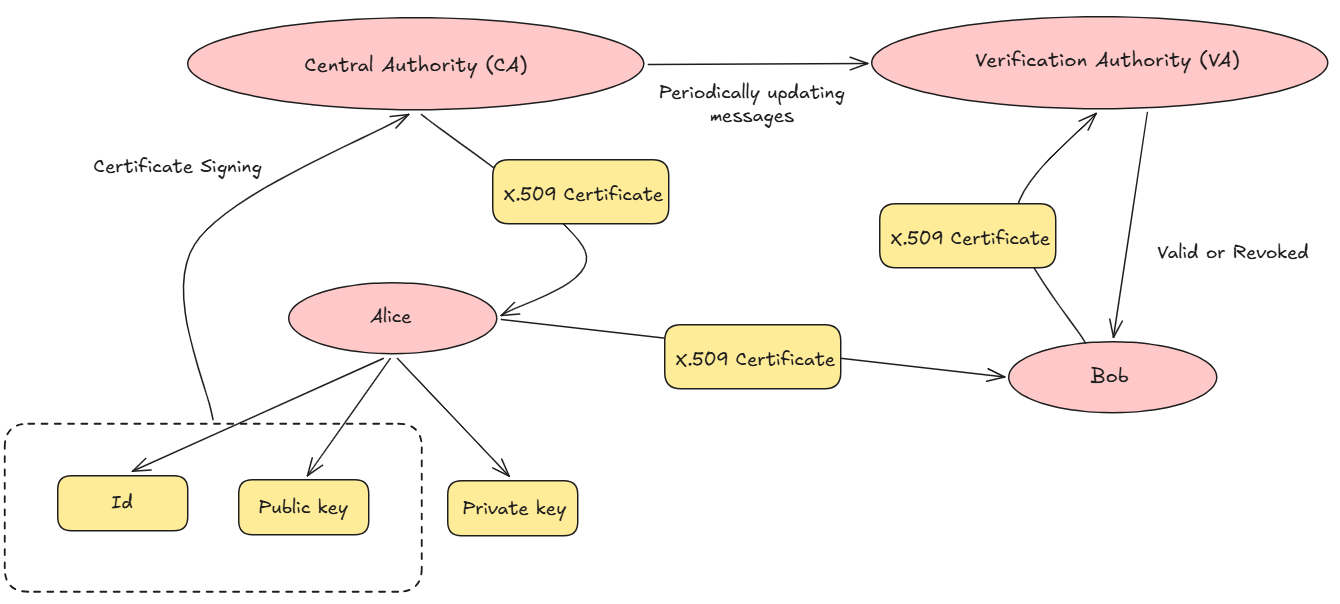
\includegraphics[width=1\linewidth]{Figure/Chap_1/PKE.png}
    \caption{Public Key Encryption paradigm}
    \label{fig:PKE}
\end{figure}


However, while PKE revolutionized secure communication, it introduced significant operational overhead in the form of public-key management, an apparatus collectively referred to as a Public Key Infrastructure (PKI). In traditional PKE infrastructures, the authenticity of a public key must be validated against a certificate issued by a CA, which means that trust does not flow directly between communicating users but is instead mediated by a hierarchy of authorities. This creates a dependency on complex certificate management, including the registration and distribution of public keys, the issuance and renewal of certificates, the maintenance and timely propagation of CRLs, and the storage and verification overhead of certificate chains. Each of these components is a potential weak point: a compromised or misbehaving CA can issue fraudulent certificates for arbitrary identities, revocation information may propagate slowly enough to leave a window of vulnerability, and the validation services themselves become availability-critical infrastructure. Consequently, users are burdened with the non-trivial task of verifying certificates before communication can proceed, which can introduce latency and additional points of failure into otherwise secure systems.


\subsection{Identity-Based Encryption}
\label{subsec:ibe}

To address these limitations, Shamir proposed identity-based cryptography (IBE), where a user’s public identity can serve directly as a public key, reducing the burden of certificate management~\cite{C:Shamir84}. Shamir’s original formulation posed this as a vision rather than a complete solution: he gave an identity-based signature scheme but left identity-based \emph{encryption} as an open problem, one that would remain unsolved for nearly two decades. The appeal of the idea is that it eliminates the indirection of certificates entirely. In environments where a centralized authority, e.g., a trusted dealer, is already present, the reliance on external certificate management becomes redundant. In particular, the core idea of IBE is that each joined party will receive secret keys bound to provided identifiers, such as a name, address, email, or blockchain wallet address. These keys are generated by a Private Key Generator (PKG) using a master public and secret key pair: the PKG publishes the master public key once, and on request derives, for any identity string, the corresponding identity-bound secret key through a key-extraction procedure. This approach streamlines key distribution by eliminating the need for certificates altogether; senders no longer need to retrieve and verify a certificate before encrypting a message. Instead, to encrypt messages so that the recipients can decrypt them correctly, senders simply provide the auxiliary information bound to the receivers, which serves as the users’ public key (Figure~\ref{fig:IBEprotocol}). Notably, a sender can even encrypt to an identity \emph{before} the corresponding secret key has been extracted, a property that proves essential in the batched, time-released setting discussed later in this chapter.

\begin{figure}[!htbp]
    \centering
    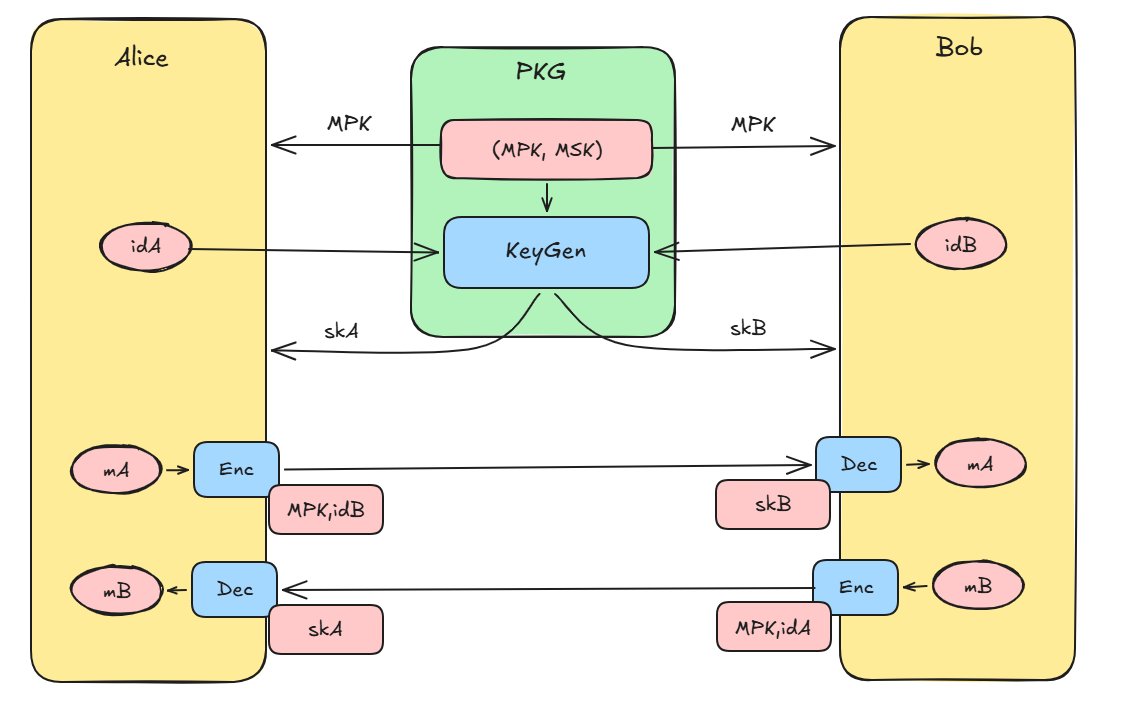
\includegraphics[width=1\linewidth]{Figure/Chap_1/IBEprotocol.png}
    \caption{The basic IBE protocol}
    \label{fig:IBEprotocol}
\end{figure}

Boneh and Franklin then gave the first practical identity-based encryption construction from bilinear pairings on elliptic curves, finally resolving Shamir’s open problem and turning IBE into a usable primitive for secure communication \cite{C:BonehFranklin01}. Their scheme demonstrated that the appealing certificate-free vision could be instantiated efficiently and with a rigorous security proof, and it triggered an extensive line of follow-up work on more expressive variants and stronger security models. The convenience of IBE, however, comes at a price that is the dual of the trust problem it solves. Because the PKG derives every user’s secret key from a single master secret, it is necessarily able to reproduce those keys itself, creating a \emph{key-escrow problem}: the authority that generates user private keys may also impersonate any user or decrypt any ciphertext addressed to them. The PKG therefore becomes a single, fully trusted point whose compromise is catastrophic for the entire system—precisely the kind of concentrated trust that distributed cryptography seeks to avoid.


\subsection{Threshold Cryptography and Distributed Trust}
\label{subsec:threshold}

Threshold cryptography addresses this weakness by distributing secret authority among multiple parties, following the principle of secret sharing introduced by Shamir, where a secret can be split into shares such that any sufficiently large subset can reconstruct it, while any smaller subset learns nothing about it \cite{M:Nakamoto08}. In a $(k, N)$ threshold scheme, the secret is encoded so that any $k$ of the $N$ shareholders can recover it but any $k-1$ of them obtain no information whatsoever, a guarantee that holds even against a computationally unbounded adversary. Applied to public-key primitives, this idea allows a private key to exist only \emph{implicitly}, as a quantity that is never reconstructed in one place: the parties instead compute the cryptographic operation, including decryption or signing, jointly, each contributing a partial result derived from its own share. Transplanting this mechanism onto the PKG of an identity-based scheme directly dissolves the key-escrow problem, since no single authority ever holds the master secret or any user’s full private key, and an adversary must corrupt an entire quorum rather than a single server to subvert the system. Thus, threshold identity-based encryption combines the usability of IBE with the robustness of distributed trust.

In standard encryption models, relying on a single, whole private key for a user creates a critical vulnerability: a single point of compromise exposes all their encrypted data. To mitigate this risk, a threshold key distribution scheme mathematically fragments the user's private key, distributing these shares across several independent parties. Under this architecture, an attacker attempting to disclose the user's private key to decrypt a targeted ciphertext cannot succeed by breaching a single location. Instead, they are forced to simultaneously compromise a predefined quorum of these independent parties to gather enough fragmented keys. This distributed approach dramatically elevates the difficulty of an attack, ensuring that the ciphertext remains entirely secure unless the specific threshold of fragments is successfully captured and reconstructed; conversely, it also improves availability, since the system continues to function as long as any qualified quorum of honest parties remains reachable, tolerating the failure or unavailability of a minority of authorities. The full construction is described in Figure~\ref{fig:thresholdIBE}. The operational flow begins with a Private Key Generator (PKG) that holds both the master public key $mpk$ and the master secret key $msk$. Rather than issuing full private keys directly, the PKG distributes secret key shares ($sk_1, sk_2, \dots, sk_N$) alongside the $mpk$ to $N$ independent parties ($P_1, \dots, P_N$). When a user requires their private key to decrypt a message, they broadcast their identity ($id$) to the network. A predefined threshold of honest parties (depicted as $P_1$ through $P_k$) process this request, generating partial identity-based secret keys ($sbk_1, \dots, sbk_k$). These partial keys are subsequently aggregated via a combine function to successfully reconstruct the pre-decryption key $sbk$. On the sender's side, a plaintext message $m$ is encrypted using the global $mpk$ and the recipient's $id$, producing the ciphertext $C_{id} = \text{Enc}(mpk, id, m)$. Finally, the recipient feeds the reconstructed $sbk$, the $mpk$, and the ciphertext into the decryption algorithm, $\text{Dec}(mpk, sbk, C_{id})$, to securely recover the original message $m$. Crucially, the most desirable instantiations of this flow are \emph{non-interactive}: each party derives its partial key locally from its own share and the requested identity, without any communication round among the authorities, so that the combine step is a simple public aggregation of independently produced shares.

\begin{figure}[h]
    \centering
    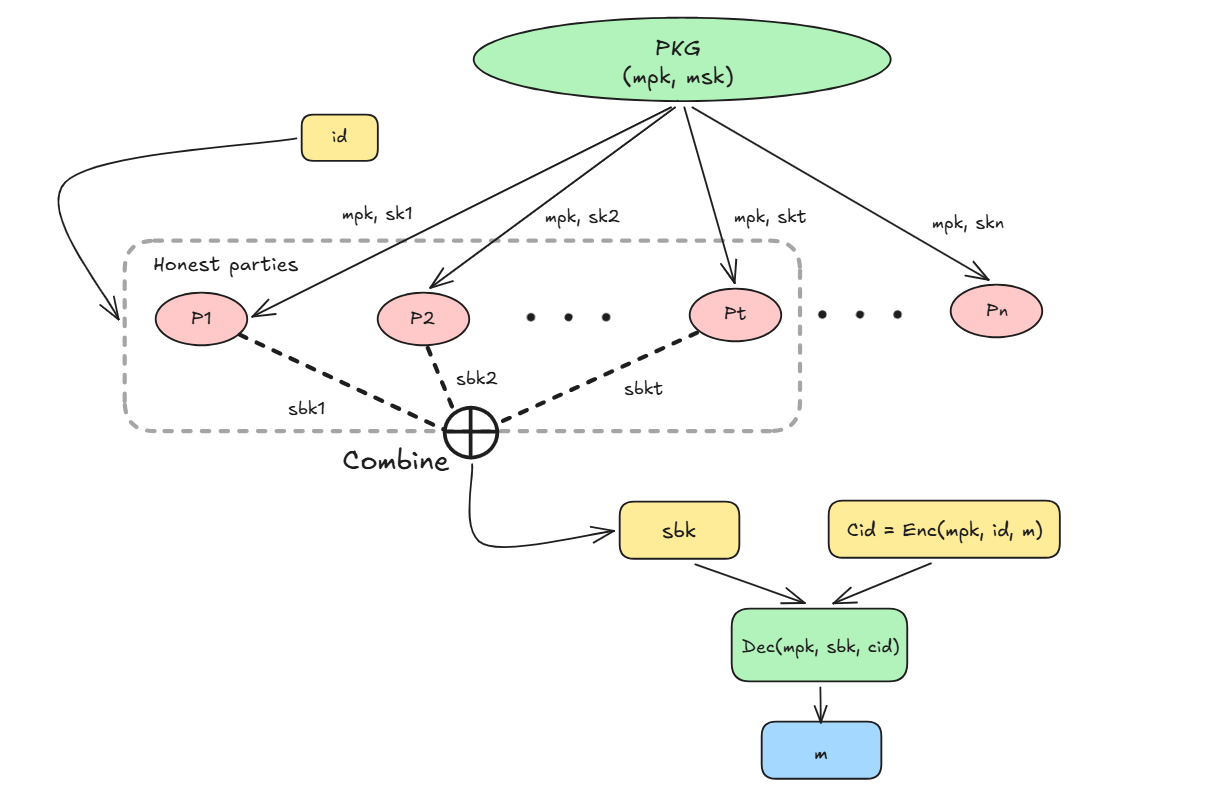
\includegraphics[width=1.1\linewidth]{Figure/Chap_1/thresholdIBE.png}
    \caption{The threshold IBE protocol}
    \label{fig:thresholdIBE}
\end{figure}


\subsection{Batched Decryption and Maximal Extractable Value}
\label{subsec:batch}

The advent of blockchain technology has brought a breakthrough in transparency, decentralization, and programmable trust, enabling a wide range of applications such as decentralized finance, digital identity, and autonomous governance. In these systems, users broadcast transactions that wait in a public holding area, the \emph{mempool}, until a block proposer selects, orders, and commits them into the next block. The same transparency that makes blockchain systems publicly verifiable, however, also introduces a new cryptographic challenge: Maximal Extractable Value (MEV). Because pending transactions are visible in the public mempool before execution, and because the party building a block enjoys near-total discretion over which transactions to include and in what order, that party can extract value by strategically positioning its own transactions relative to those of ordinary users. Concretely, this ordering power enables front-running (placing a transaction just ahead of a victim’s), back-running (placing one just behind it), sandwich attacks (surrounding a victim’s trade on both sides), and selective inclusion or censorship of transactions~\cite{SP:Daian20}. This issue is particularly harmful in decentralized finance, where the outcome and value of a transaction may depend heavily on its position within a block, so that the same trade can yield a materially worse price purely because of how it was ordered (Figure~\ref{fig:MEV}). 


\begin{figure}[!h]
    \centering
    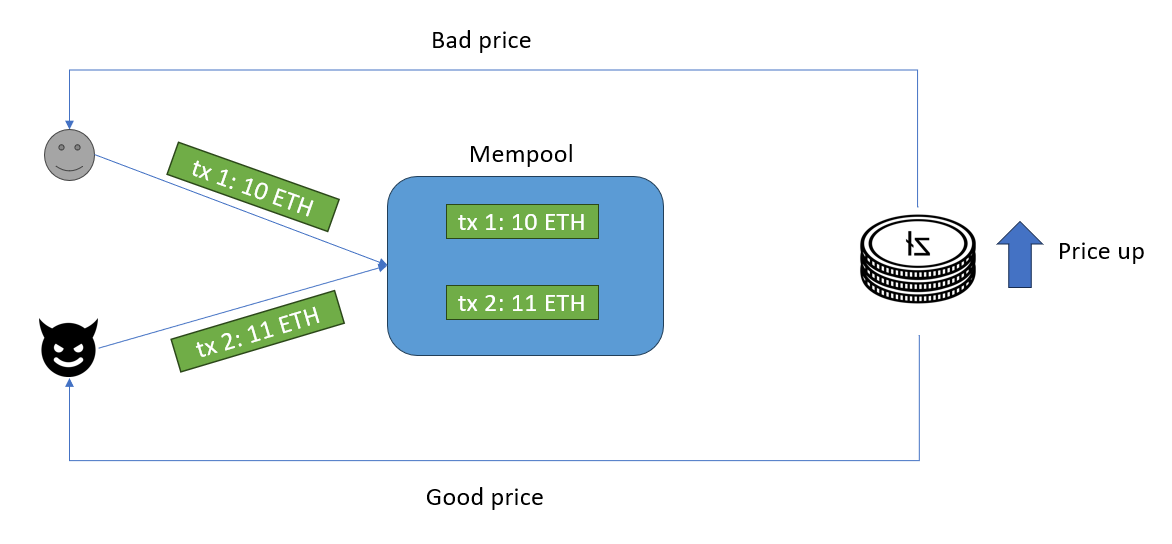
\includegraphics[width=1.0\linewidth]{Figure/Chap_1/MEV.png}
    \caption{Illustration of MEV attack}
    \label{fig:MEV}
\end{figure}

Beyond the direct financial harm to users, the competition to capture MEV exerts destabilizing pressure on the consensus layer itself and encourages centralization of block production. Existing mitigations, such as private relays and private mempools, can reduce public transaction exposure, but they often shift trust to specialized intermediaries instead of eliminating the underlying ordering-information asymmetry. Therefore, a more principled cryptographic solution is needed: transaction contents should remain hidden until their ordering has already been fixed.

This motivates the rise of threshold batch identity-based encryption as a direct defense against MEV. In this approach, users encrypt their transactions before broadcasting them, while the capability to decrypt is distributed among a committee of validators or key authorities. No single party can decrypt early; only after a transaction batch has been ordered or finalized can a threshold of participants jointly release the decryption material, so that block builders are forced to commit to an ordering while still blind to the contents they are ordering. The identity-based structure makes this mechanism especially natural for blockchain settings: the encryption identity can encode a block number, epoch, application, auction round, or transaction batch label, so that ``the right to decrypt this slot'' is exactly the identity-bound key the committee releases for that slot. The \emph{batch} requirement reflects a practical efficiency concern: a block contains many transactions, and performing an independent threshold decryption for each one would be prohibitively expensive, so the goal is to release decryption for an entire batch at amortised cost. The first concrete construction in this line was proposed in \cite{EPRINT:BonLauTas25}, which combines a KZG polynomial commitment scheme with an efficient special-purpose witness encryption scheme. Its security model is comparatively weak, however, since it is proven in the generic group model. Several concurrent works have since attempted to overcome the remaining limitations and produce more concrete and efficient schemes. Boneh et al. propose an efficient BTE construction based on partial-fraction techniques, showing that algebraic batching can reduce decryption overhead while supporting short-ciphertext variants and practical implementations \cite{EPRINT:BNRT26}. Building on this direction, Agarwal et al. introduce BTX, a simpler and concretely efficient BTE scheme that is both epochless and collision-free and avoids user-chosen ciphertext indices~\cite{EPRINT:ADGRS26}.


\subsection{Toward Post-Quantum Threshold Batch IBE}
\label{subsec:pq-tbibe}

Unfortunately, despite being conceptually simple and practically efficient, all the aforementioned schemes rest on the elliptic-curve pairing assumption, whose underlying discrete-logarithm hardness is devastatingly broken by Shor’s algorithm, which solves both integer factorization and discrete logarithms in polynomial time on a quantum computer \cite{J:Shor97}. This threat is not merely asymptotic: an adversary can harvest encrypted traffic today and decrypt it once a sufficiently capable quantum machine becomes available, which is especially damaging for blockchains, where ciphertexts and commitments are recorded permanently and publicly. The cryptographic community has responded with a sustained effort to migrate to assumptions believed to resist quantum attack, and among the candidate families, lattice-based schemes have gained the broadest popularity due to their well-established post-quantum security guarantees, their reductions from worst-case lattice problems, and their versatility in supporting advanced functionalities. The security of these schemes typically reduces to the Learning With Errors (LWE) and Short Integer Solution (SIS) problems, and their most powerful constructions are enabled by \emph{lattice trapdoors}: short secret bases that permit sampling short preimages of a public matrix, the very mechanism underlying lattice-based identity-based encryption and signatures.

From this motivation, Boneh et al. \cite{EPRINT:BonLauTas25} constructed a new lattice-based batched decryption scheme, utilizing an explainable sampler and a shifted multi-preimage trapdoor sampler. More recently, Xiong, Zhang, and Chen proposed the first batched IBE from lattices in the standard model, proving security under the succinct LWE assumption \cite{EPRINT:XioChe25}. Yet making such schemes \emph{threshold} runs into a fundamental obstacle: finding an effective way to secret share the lattice trapdoor, which is the fundamental building block of essentially all lattice-based primitives, remains a non-trivial task. The difficulty is structural—a lattice trapdoor is a short basis whose usefulness depends delicately on its smallness, so naively splitting or summing trapdoor material tends either to destroy the shortness that makes it a trapdoor or to leak information about it. Prior approaches to thresholdizing lattice-based trapdoor primitives either rely on generic tools, such as the universal thresholdizer based on threshold FHE~\cite{BGG+18,ASY22}, or on MPC-based trapdoor-sharing techniques~\cite{BKP13}; however, these methods are concretely expensive, require heavy interaction between the parties, or depend on precomputed correlated randomness, none of which fits the non-interactive, public-aggregation flow desired in the mempool setting. A separate line of work develops tailored lattice-based threshold signatures~\cite{GKS24,DKM+24,EKT24,BKL+25}, but these constructions are usually interactive and rely on the specific structure of the underlying $\Sigma$-protocol, making them difficult to repurpose for general trapdoor-based primitives such as IBE. Related notions such as half trapdoors~\cite{Wee21} and subspace trapdoors~\cite{PT24} provide only weaker or different functionalities, and do not by themselves yield a distributed preimage sampler. In contrast, partial lattice trapdoors offer a direct algebraic mechanism for non-interactively distributing lattice preimage sampling: each party holds a partial trapdoor, samples a partial preimage locally, and the partial preimages recombine into a valid short preimage by simple summation, thereby giving a plug-and-play route toward threshold versions of trapdoor-based primitives such as signatures and identity-based encryption. It is precisely this primitive that the present thesis builds upon to obtain a post-quantum, non-interactive threshold batch IBE.


% \section{Related work}


\section{Our results}
\label{section:1.2}
This thesis set out to answer a concrete and timely question: \emph{can the
batched decryption used in encrypted mempools be made both post-quantum and
trustless at the same time?} Existing batch threshold encryption schemes achieve
the trustless property but rely on pairing-based assumptions that do not survive
quantum adversaries, while the lattice machinery that would make them
post-quantum, namely trapdoor preimage sampling, has long resisted efficient,
non-interactive thresholdization. The central contribution of this thesis is a
construction that resolves this tension: a lattice-based threshold batch
identity-based encryption (\textsf{TBIBE}) scheme in which decryption authority
is split $k$-out-of-$N$ across a committee, without any interaction between the
parties at decryption time.
 
Concretely, the work of this thesis can be summarized in the following
contributions.
 
\begin{enumerate}
    \item \textbf{A new post-quantum threshold batch IBE scheme.}
    We design a $k$-out-of-$N$ threshold batch IBE by combining the index-dependent
    batched decryption scheme of Boneh, Laufer and Tas~\cite{EPRINT:BonLauTas25}
    with the partial lattice trapdoors of Albrecht, Lai, Lapiha and
    Woo~\cite{AC:ALLW25}. The key technical step is to replace the single
    $\mathsf{SamplePre}$ call that produces the batch pre-decryption key
    $\mathsf{sbk}$ with its distributed analogue $\mathsf{PSampPre}$ followed by
    reconstruction $\mathsf{Rec}$, so that each authority holds only a partial
    trapdoor $\mathsf{ptd}_j$, locally emits a partial key $\mathsf{sbk}_j$, and any
    qualified quorum recombines these shares into the full key by simple summation.
    To our knowledge, this is the first construction to thresholdize a lattice-based
    \emph{batched} IBE in this purely algebraic, non-interactive way.
 
    \item \textbf{A formal syntax and security model for $\mathsf{TBIBE}$.}
    We give a precise five-algorithm syntax
    ($\mathsf{Setup}$, $\mathsf{Enc}$, $\mathsf{PreDec}$, $\mathsf{Combine}$,
    $\mathsf{Dec}$) and a correctness definition for the threshold setting, and we
    introduce a \emph{highly selective} security notion that faithfully captures
    what the secret-sharing layer permits an adversary to learn, including the
    corruption of up to $k-1$ parties and the release of all but one partial key
    for the challenge quorum.
 
    \item \textbf{Correctness and security proofs.}
    We prove correctness from the structural properties of the shifted
    multi-preimage sampler, the explainable $\mathsf{SampleLeft}$ procedure, and the
    reconstruction guarantee of the partial trapdoor scheme. We then prove security
    through an explicit sequence of hybrid games that reduces the advantage of any
    efficient adversary to the
    $(nk, 2mk, \chi_0, \chi_1, \sigma_2)$-indistinguishability of the partial
    trapdoor, and hence to the $\kappa$-LWE assumption (with one-wayness resting on
    $\kappa$-SIS), closing the remaining gaps with Gaussian-smoothing and
    noise-flooding arguments.
 
    \item \textbf{A unified treatment and analysis of the building blocks.}
    We assemble and present, in a single consistent framework, the lattice
    tools the construction depends on, gadget and Ajtai trapdoors, the explainable
    sampler, the shifted multi-preimage trapdoor sampler, and partial lattice
    trapdoors, and we adapt their correctness and hardness statements to the
    dimensions used by our scheme.
 
    \item \textbf{An efficiency study and proof-of-concept evaluation.}
    We derive the asymptotic sizes of the public key, ciphertext, and pre-decryption
    key, analyze the runtime of each algorithm, and identify the pre-decryption phase
    (explainable $\mathsf{SampleLeft}$ and $\mathsf{PSampPre}$) as the dominant cost.
    A proof-of-concept implementation under representative parameters demonstrates
    that the scheme is feasible and isolates the concrete bottlenecks that future
    optimization should target.
\end{enumerate}
 
Taken together, these contributions show that partial lattice trapdoors are an
effective and practical tool for distributing decryption authority in
lattice-based identity-based encryption. The resulting scheme inherits the most
valuable property of its underlying trapdoor-sharing mechanism, namely that the
distribution of the decryption capability is fully \emph{non-interactive}: parties
never communicate to produce their shares, which sets the construction apart from
prior thresholdization routes based on threshold FHE or multiparty computation.




\label{section:1.4}

\section{Thesis Organization}

The remainder of this thesis is organized as follows.

\begin{itemize}
    \item \textbf{Chapter~2} presents the necessary preliminaries for the proposed construction. 
    It reviews fundamental lattice theory, lattice-based hardness assumptions, gadget and 
    Ajtai trapdoors, explainable sampler, shifted multi-preimage trapdoor 
    samplers, and partial lattice trapdoors.

    \item \textbf{Chapter~3} introduces the proposed threshold batch identity-based encryption 
    construction. It first defines the syntax of the scheme and then describes the setup, 
    encryption, partial pre-decryption, key-combination, and decryption algorithms in detail.

    \item \textbf{Chapter~4} analyzes the correctness and security of the proposed construction. 
    It proves that the decryption procedure correctly recovers the encrypted messages under 
    the chosen parameters, derives the asymptotic sizes of the main objects, and establishes 
    security in the highly selective model through a sequence of hybrid games.

    \item \textbf{Chapter~5} discusses the experimental evaluation of the proposed scheme, 
    including implementation considerations and the efficiency of the main algorithms.

    \item \textbf{Chapter~6} concludes the thesis by summarizing the main contributions and 
    discussing possible directions for future work.

    \item \textbf{Appendix} provides additional technical details, including the shifted 
    multi-preimage trapdoor sampler, the construction of $\mathsf{SampleLeft}$, the explainable 
    $\mathsf{SampleLeft}$ procedure, and the partial gadget trapdoor construction.
\end{itemize}


% \end{document} % Phần mở đầu

\newpage
%\pagestyle{fancy} % Áp dụng header và footer
\chapter{Preliminaries}
% \documentclass[../main.tex]{subfiles}
% \begin{document}

\textbf{Notation.}
We denote by $\lambda$ the security parameter.
A function $f$ is \emph{negligible} in $\lambda$, denoted by $\mathrm{negl}(\lambda)$, if
$f(\lambda) < 1/\mathrm{poly}(\lambda)$ for every polynomial $\mathrm{poly}(\lambda)$ as $\lambda \to \infty$.
Computationally and statistically indistinguishable games are denoted by $\approx_c$ and $\approx_s$, respectively.
We denote the set $\{1,\dots,n\}$ by $[n]$, and the sequence $(x_{a_1}, \dots, x_{a_k})$ with
$a_1 < \cdots < a_k$ by $(x_{a_i})_{a_i \in \{a_1,\dots,a_k\}}$.
A positive semidefinite matrix $\mathbf{\Sigma}$ can be written as
$\mathbf{\Sigma} = \mathbf{S}\mathbf{S}^t$.
Therefore, we use $\sqrt{\mathbf{\Sigma}}$ to denote any fixed matrix $\mathbf{S}$ satisfying the above relation.

\section{Fundamental Lattice Theory}

\begin{definition}
Let $\mathbf{A} = [\mathbf{a}_1,\mathbf{a}_2,\dots,\mathbf{a}_m] \in \mathbb{R}^{n\times m}$ be a matrix whose columns are linearly independent.
The lattice generated by these vectors is defined as
\[
\Lambda(\mathbf{A})
=
\left\{
\sum_{i=1}^{m} z_i \mathbf{a}_i \,\middle|\, z_i \in \mathbb{Z}\ \forall i \in [m]
\right\}.
\]
The set $\{\mathbf{a}_1,\mathbf{a}_2,\dots,\mathbf{a}_m\}$ is called a basis of the lattice.
\end{definition}

\begin{definition}
Let $n,m,q$ be positive integers and let $\mathbf{A}\in\mathbb{Z}_q^{n\times m}$.
We define the following $m$-dimensional $q$-ary lattices associated with $\mathbf{A}$:
\[
\setlength{\jot}{2pt}
\begin{aligned}
\Lambda^\perp(\mathbf{A})
&=
\left\{
\mathbf{z}\in\mathbb{Z}^m : \mathbf{A}\mathbf{z}\equiv \mathbf{0}\pmod q
\right\},\\
\Lambda(\mathbf{A}^t)
&=
\left\{
\mathbf{v}\in\mathbb{Z}^m : \exists\,\mathbf{s}\in\mathbb{Z}_q^n \text{ such that } \mathbf{v}\equiv \mathbf{A}^t\mathbf{s}\pmod q
\right\},\\
\Lambda^{\mathbf{u}}(\mathbf{A})
&=
\left\{
\mathbf{v}\in\mathbb{Z}^m : \mathbf{A}\mathbf{v}\equiv \mathbf{u}\pmod q
\right\}
=
\mathbf{x} + \Lambda^\perp(\mathbf{A}),
\end{aligned}
\]
for $\mathbf{u} \in \mathbb{Z}_q^n$, where $\mathbf{x}\in\mathbb{Z}^m$ is any solution satisfying
$\mathbf{A}\mathbf{x}\equiv \mathbf{u}\pmod q$.
\end{definition}

Dual lattices play a central role in the analysis of Gaussian meansure, which is essential for the security proof of every cryptographic scheme


\begin{definition}
For a lattice $\Lambda$, we define the \emph{dual lattice}
$\Lambda^* = \{\mathbf{w} \in \mathbb{R}^n : \forall \mathbf{x} \in \Lambda,\ \mathbf{w}^{\top}\mathbf{x} \in \mathbb{Z}\}$.
\end{definition}
\noindent For all the matrix $\mathbf{A} \in \mathbb{Z}_q^{n \times m}$, it holds that $\Lambda(\mathbf{A}) = q \cdot \Lambda^\perp(\mathbf{A})^*$. Indeed, if we take $\mathbf{x} \in \Lambda(\mathbf{A})$, then for any $\mathbf{y} \in \Lambda^\perp(\mathbf{A})$, we have $\big \langle \dfrac{\mathbf{x}^\top}{q},\mathbf{y}\big\rangle= \big \langle \dfrac{\mathbf{z}^\top\mathbf{A}}{q},\mathbf{y}\big\rangle = \big \langle \dfrac{\mathbf{z}^\top}{q},\mathbf{A}\mathbf{y}\big\rangle=\big \langle \dfrac{\mathbf{z}^\top}{q},\mathbf{k}q\big\rangle =\big \langle \mathbf{z}^\top,\mathbf{k}\big\rangle \in \mathbb{Z}$ where $\mathbf{z}$ and $\mathbf{k}$ all come from $\mathbb{Z}^n$. And since this also holds for every $\mathbf{x} \in \Lambda(\mathbf{A})$, we have the desired result. 

For a lattice $\Lambda$, the smoothing parameter $\eta_{\varepsilon}(\Lambda)$ denotes the smallest Gaussian parameter $s$ such that the Gaussian mass over the nonzero dual lattice vectors becomes negligible, i.e.,
\[
\rho_{1/s}(\Lambda^* \setminus \{\mathbf{0}\}) \le \varepsilon.
\]
This parameter is a standard tool in lattice-based cryptography for analyzing discrete Gaussian sampling ~\cite{J:MicReg07}.

\begin{lemma}[From~\cite{C:GenPeiVai08}]
\label{lem:1}
For any $n$-dimensional lattice $\Lambda$ and real $\epsilon > 0$ and $\mathbf{S} \subset \Lambda$ is a basis of it, we have
\[
\eta_{\epsilon}(\Lambda)
\leq
\|\widetilde{S}\|
\cdot
\sqrt{\log(2n(1+1/\epsilon))/\pi}.
\]
Then, for any $\omega(\sqrt{\log n})$ function, there is a negligible
$\epsilon(n)$ for which
$
\eta_{\epsilon}(\Lambda)
\leq
\|\widetilde{S}\|\cdot \omega(\sqrt{\log n}).
$
\end{lemma}

\begin{lemma}[Gaussian Tail Bound~\cite{C:MicPei12}]
\label{lem:2}
Let $\mathbf{B} \in \mathbb{R}^{n \times n}$ be a full-rank basis and let
$\Lambda$ be the $n$-dimensional lattice generated by $\mathbf{B}$.
Suppose $s \ge \eta_{\varepsilon}(\Lambda)$ for some
$\varepsilon \in (0,1)$. Then, for all $\mathbf{c} \in \mathbb{R}^n$,
\[
\Pr\left[
    \|\mathbf{v}\| > s\sqrt{n}
    :
    \mathbf{v} \leftarrow \mathcal{D}_{\Lambda+\mathbf{c},s}
\right]
\le
2^{-n}\cdot \frac{1+\varepsilon}{1-\varepsilon}.
\]
\end{lemma}


\begin{definition}[Tensor Product / Kronecker Product]
Let $\mathbf{A} = (a_{i,j}) \in \mathbb{Z}^{n \times m}$ and $\mathbf{B} \in \mathbb{Z}^{\ell \times \lambda}$. The tensor product, also called the Kronecker product, of $\mathbf{A}$ and $\mathbf{B}$ is defined as
\[
\mathbf{A} \otimes \mathbf{B}
=
\begin{bmatrix}
a_{1,1}\mathbf{B} & \cdots & a_{1,m}\mathbf{B} \\
\vdots & \ddots & \vdots \\
a_{n,1}\mathbf{B} & \cdots & a_{n,m}\mathbf{B}
\end{bmatrix}
\in \mathbb{Z}^{n\ell \times m\lambda}.
\]
\end{definition}

The Kronecker product satisfies the following mixed-product property:
\[
(\mathbf{A} \otimes \mathbf{B})(\mathbf{C} \otimes \mathbf{D})
=
(\mathbf{A}\mathbf{C}) \otimes (\mathbf{B}\mathbf{D}),
\]
whenever the matrix products $\mathbf{A}\mathbf{C}$ and $\mathbf{B}\mathbf{D}$ are well-defined.

\begin{definition}
The $n$-dimensional Gaussian function is defined as
\[
\rho_{\mathbf{B},\mathbf{c}}(\mathbf{x})
=
\rho_{\sqrt{\mathbf{\Sigma}},\mathbf{c}}(\mathbf{x})
=
\exp\!\left(
-\pi (\mathbf{x}-\mathbf{c})^t \mathbf{\Sigma}^{-1} (\mathbf{x}-\mathbf{c})
\right),
\]
for invertible $\mathbf{B}\in\mathbb{R}^{n\times n}$, $\mathbf{c}\in\mathbb{R}^n$, and
$\mathbf{\Sigma}:=\mathbf{B}\mathbf{B}^t$.
When $\mathbf{\Sigma}=\sigma^2\mathbf{I}$ and $\mathbf{c}=\mathbf{0}$, we write $\rho_\sigma$.
\end{definition}

\begin{definition}
The discrete Gaussian distribution over $\Lambda$ with parameter $\sqrt{\mathbf{\Sigma}}$ and center $\mathbf{c}$ is defined as
\[
\mathcal{D}_{\Lambda,\mathbf{\Sigma},\mathbf{c}}(\mathbf{x})
=
\frac{\rho_{\sqrt{\mathbf{\Sigma}},\mathbf{c}}(\mathbf{x})}
{\sum_{\mathbf{y}\in\Lambda}\rho_{\sqrt{\mathbf{\Sigma}},\mathbf{c}}(\mathbf{y})}
=
\frac{\rho_{\sqrt{\mathbf{\Sigma}},\mathbf{c}}(\mathbf{x})}
{\rho_{\sqrt{\mathbf{\Sigma}},\mathbf{c}}(\Lambda)}.
\]
\end{definition}

\begin{definition}
    Let $X, Y$ are two discrete random variables over countable set $A$. The statistical distance between them is defined as 
    $$
    \triangle[X,Y] = \dfrac{1}{2}\sum_{a \in A}|\Pr\{X=a\}-\Pr\{X=b\}|
    $$
\end{definition}



\begin{lemma}[Leftover Hash Lemma~\cite{SIComp:HILL99}]
\label{lem:leftoverHash}
Let $n,m,q$ be lattice parameters, and suppose $m \ge 2n \log q$ and $q > 4$. Then, the statistical distance between the following distributions is at most $2^{-n}$:
\[
\left\{(\mathbf A,\mathbf A\mathbf x) : \mathbf A \xleftarrow{\$} \mathbb Z_q^{n\times m},\ \mathbf x \xleftarrow{\$} \{0,1\}^m \right\}
\quad \text{and} \quad
\left\{(\mathbf A,\mathbf y) : \mathbf A \xleftarrow{\$} \mathbb Z_q^{n\times m},\ \mathbf y \xleftarrow{\$} \mathbb Z_q^n \right\}.
\]

\end{lemma}
\begin{proof}
Let us define
$S_{\mathbf A}(\mathbf y)=\{\mathbf x \in \{0,1\}^m : \mathbf A\mathbf x=\mathbf y\}$
for a fixed matrix $\mathbf A$. Hence, the statistical distance between the given distributions is
$$
\begin{aligned}
\Delta
=
\mathbb E_{\mathbf A}
\left[
\sum_{\mathbf y \in \mathbb Z_q^n}
\left|
\dfrac{|S_{\mathbf A}(\mathbf y)|}{2^m}
-
\dfrac{1}{q^n}
\right|
\right]
&\leq
\mathbb E_{\mathbf A}
\left[
\sqrt{
q^n
\sum_{\mathbf y \in \mathbb Z_q^n}
\left(
\dfrac{|S_{\mathbf A}(\mathbf y)|}{2^m}
-
\dfrac{1}{q^n}
\right)^2
}
\right]
\\
&=
\mathbb E_{\mathbf A}
\left[
\sqrt{
q^n
\left(
\dfrac{1}{2^{2m}}
\sum_{\mathbf y \in \mathbb Z_q^n}
|S_{\mathbf A}(\mathbf y)|^2
-
\dfrac{1}{q^n}
\right)
}
\right],
\end{aligned}
$$
where the last equality follows from $\sum_{\mathbf y \in \mathbb Z_q^n}
|S_{\mathbf A}(\mathbf y)|
=
2^m.$

Assume we have $\mathbf x,\mathbf x' \in \{0,1\}^m$ and let
$\mathbf z = \mathbf x-\mathbf x' \in \{-1,0,1\}^m$.
We know that
$$
\Pr_{\mathbf A}
\left[
\mathbf A\mathbf z = \mathbf 0
:
\mathbf z \in \{-1,0,1\}^m,\ \mathbf z \neq \mathbf 0
\right]
=
\dfrac{1}{q^n}.
$$
Indeed, since $\mathbf z \neq \mathbf 0$, there exists some index $j$ such that $z_j=\pm 1$.
We fix all columns of $\mathbf A$ except for the $j$-th column and then average over the remaining one.
Since $z_j=\pm 1$ is invertible modulo $q$, the previous claim follows.

We note that
$
\sum_{\mathbf y \in \mathbb Z_q^n}
|S_{\mathbf A}(\mathbf y)|^2
=
\left|
\left\{
(\mathbf x,\mathbf x')
:
\mathbf A\mathbf x = \mathbf A\mathbf x'
\right\}
\right|.
$
Hence, taking the expectation over $\mathbf A$ gives:
$$
\begin{aligned}
\mathbb E_{\mathbf A}
\left[
\sum_{\mathbf y \in \mathbb Z_q^n}
|S_{\mathbf A}(\mathbf y)|^2
\right]
&=
2^m
+
\Pr_{\mathbf A}
\left[
\mathbf A\mathbf x=\mathbf A\mathbf x'
:
\mathbf x,\mathbf x' \in \{0,1\}^m,\ \mathbf x \neq \mathbf x'
\right]
\cdot
(2^{2m}-2^m)
\\
&=
2^m
+
\dfrac{2^{2m}-2^m}{q^n}.
\end{aligned}
$$

From this, we have
$$
\begin{aligned}
\Delta
&\leq
\sqrt{
q^n
\left(
\dfrac{1}{2^{2m}}
\left(
2^m+\dfrac{2^{2m}-2^m}{q^n}
\right)
-
\dfrac{1}{q^n}
\right)
}
\\
&=
\sqrt{
q^n
\left(
\dfrac{1}{2^m}
-
\dfrac{1}{2^m q^n}
\right)
}
\\
&\leq
\sqrt{\dfrac{q^n}{2^m}}
\\
&\leq
\dfrac{1}{q^{n/2}}
\\
&\leq
2^{-n},
\end{aligned}
$$
where the last inequality follows from $q>4$. This completes the proof.
\end{proof}

\begin{lemma}[Regularity Lemma~\cite{C:GenPeiVai08}]
\label{lem:4}
Let $n$ be a positive integer, let $q$ be a prime, and let
$m \ge 2n\log q$. Then, for all but a negligible fraction of
$\mathbf{A} \in \mathbb{Z}_q^{n\times m}$, and for any
$\sigma \ge \omega(\sqrt{\log m})$, we have 
$$\{\mathbf{Ae} \mod q:e \leftarrow \mathcal{D}_{\mathbb{Z}^m,\sigma}\} \approx_s \mathbf{U}_\mathbb{Z_q^n}$$
\end{lemma}


\begin{lemma}[From~\cite{EC:CasHofKilPei10}, adapted from Lemma~16~\cite{EPRINT:BonLauTas25}]
\label{lem:tail_bound}
Let $q \geq 2$ and $\mathbf{A} \in \mathbb{Z}_q^{n \times m}$ be a matrix
with $m > n$. Then, for $\mathbf{u} \in \mathbb{Z}_q^n$, it holds that
\[
    \Pr\left[
        \|\mathbf{x}\| > \sqrt{m}\sigma
        :
        \mathbf{x} \leftarrow \mathbf{A}_{\sigma}^{-1}(\mathbf{u})
    \right]
    \leq \operatorname{negl}(n).
\]
\end{lemma}

\begin{lemma}[From~\cite{C:MicPei12}]
\label{lem:gaget_matrix_sam}
For any integers $q \geq 2$, $n \geq 1$, $k = (\lceil \log q \rceil + 1)$ and $m = nk$, there is a primitive matrix
$\mathbf{G} \in \mathbb{Z}_q^{n \times m}$ such that the lattice $\Lambda^\perp(\mathbf{G})$ has a known basis $\mathbf{S} \in \mathbb{Z}^{m \times m}$ with $\|\widetilde{\mathbf{S}}\| \leq \sqrt{5}$ and $\|\mathbf{S}\| \leq \max\{\sqrt{5}, \sqrt{k}\}$.
\end{lemma}

\begin{lemma}[From~\cite{C:GenPeiVai08}]
\label{lem:uniform_mul_gaussian}
Let $n$ and $q$ be positive integers, where $q$ is prime, and let
$m \geq 2n\log q$. Then, except for at most a $2q^{-n}$ fraction of
matrices $\mathbf{A} \in \mathbb{Z}_q^{n \times m}$, for every
$s \geq \omega(\sqrt{\log m})$, the syndrome
$
\mathbf{u} = \mathbf{A}\mathbf{e} \bmod q
$
is statistically close to the uniform distribution over $\mathbb{Z}_q^n$,
where $\mathbf{e} \leftarrow D_{\mathbb{Z}^m,s}$.
\end{lemma}

\begin{lemma}[From~\cite{C:GenPeiVai08}]
\label{lem:5}
Let $n$ be a positive integer, let $q$ be a prime, and let
$m' = n(\lceil \log q \rceil + 1)$. For any
$\sigma \geq \omega(\sqrt{\log m'})$, if
$\mathbf{v} \leftarrow \mathbb{Z}_q^n$ and
$\mathbf{u} \leftarrow \mathbf{G}_{\sigma}^{-1}(\mathbf{v})$, then
$\mathbf{u}$ is statistically close to
$D_{\mathbb{Z}^{m'},\sigma}$.
\end{lemma}
\begin{proof}
By lemma~\ref{lem:1}, the smoothing pararamter $\eta_{\varepsilon}(\Lambda^\perp(\mathbf{G}) \leq \sqrt{5}\cdot \omega(\sqrt{\log n})$, which immediately implies that $\sigma \geq \eta_{\varepsilon}(\Lambda^\perp(\mathbf{G}))$. Finally, note that the columns of $\mathbf{G}$ generate $\mathbb{Z}_q^n$, by Lemma~\ref{lem:gaget_matrix_sam}, we derive the desirable result.
\end{proof}
\section{Hard Assumptions}

\begin{definition}[Learning with Errors -- LWE]

Ever since the first formal reduction from worst case to average case by Regev~\cite{J:Regev09}, Learning with Errors (LWE) has seen an intensive adoption and become a crucial building block of several cryptographic primitives.
At its core, LWE can be viewed as a \emph{noisy} linear algebra problem. In standard (noiseless) linear algebra over $\mathbb{Z}_q$, given a matrix $\mathbf{A} \in \mathbb{Z}_q^{m \times n}$ and a vector $\mathbf{b} = \mathbf{A}\mathbf{s}$, one can recover the secret $\mathbf{s} \in \mathbb{Z}_q^n$ by Gaussian elimination. LWE makes this computationally intractable by adding a small random error: the adversary sees $\mathbf{b} = \mathbf{A}\mathbf{s} + \mathbf{e}$, where $\mathbf{e}$ is a noise vector drawn from an error distribution $\chi$ (typically a discrete Gaussian $\mathcal{D}_{\mathbb{Z},\sigma}$ with $\sigma \ll q$). The noise is large enough to defeat algebraic attacks yet small enough relative to $q$ that it does not destroy the useful structure needed for cryptographic constructions.

Two hardness variants are studied. The \emph{search} variant asks to recover $\mathbf{s}$ given arbitrarily many samples $(\mathbf{a}_i, \mathbf{a}_i^\top\mathbf{s} + e_i)$. The \emph{decisional} variant, which suffices for the constructions in this thesis, asks only to \emph{distinguish} such samples from uniformly random pairs. Regev~\cite{J:Regev09} proved a (quantum) reduction from worst-case lattice problems (GapSVP and SIVP) to average-case decisional LWE, grounding its hardness in a well-studied geometric problem.

Formally, given a prime $q$, a positive integer $n$, and a distribution $\chi$ over $\mathbb{Z}_q$, the
$\mathrm{LWE}_{\mathbb{Z}_q,n,\chi}$ problem instance is associated with a challenge oracle $\mathcal{O}$ that behaves as follows:
\begin{itemize}
    \item $\mathcal{O}_{\mathbf{s}}$ outputs samples of the form
    $(\mathbf{u}_i,v_i):=(\mathbf{u}_i,\mathbf{u}_i^t \mathbf{s}+x_i)\in \mathbb{Z}_q^n\times \mathbb{Z}_q,$
    where $\mathbf{u}_i\leftarrow \mathbb{Z}_q^n$, $\mathbf{s}\leftarrow \mathbb{Z}_q^n$ is a uniformly random secret, and
    $x_i\in \mathbb{Z}_q$ is a fresh sample from $\chi$.

    \item $\mathcal{O}_{\Phi}$ outputs uniformly random samples from $\mathbb{Z}_q^n\times \mathbb{Z}_q$.
\end{itemize}

An algorithm $\mathcal{A}$ decides the $(\mathbb{Z}_q,n,\chi)$-LWE problem if, for some
$\mathbf{s}\leftarrow \mathbb{Z}_q^n$, the advantage of $\mathcal{A}$, defined as
\[
\mathrm{Adv}_{\mathrm{LWE}}[\mathcal{A}]
=
\left|
\Pr[\mathcal{A}^{\mathcal{O}_{\mathbf{s}}}=1]
-
\Pr[\mathcal{A}^{\mathcal{O}_{\Phi}}=1]
\right|,
\]
is non-negligible in $\lambda$.
\end{definition}

\begin{definition}[$\kappa$-Uniform Distribution~\cite{AC:ALLW25}]
Let $\varphi,\kappa,m,\log q \in \mathrm{poly}(\lambda)$ with $\kappa \le m$.
For any $\mathbf{U} \in \mathbb{Z}_q^{m\times \kappa}$, denote
$\mathbf{U}^{\perp} = \left\{\mathbf{x} \in \mathbb{Z}_q^m : \mathbf{x}^t \cdot \mathbf{U} = \mathbf{0}^t \bmod q \right\}.$
The $\kappa$-uniform distribution with parameters $\mathbf{U},\mathbf{R},q,\chi$ is
\[
\mathcal{U}(\mathbf{U}^{\perp}) + \mathcal{D}_{\mathbb{Z},\chi}^{m}
:=
\left\{
\mathbf{b}
\;\middle|\;
\mathbf{x}\leftarrow \mathbf{U}^{\perp};
\;
\mathbf{e}\leftarrow \mathcal{D}_{\mathbb{Z},\chi}^{m};
\;
\mathbf{b}:=\mathbf{x}+\mathbf{e}
\right\}.
\]
\end{definition}

\begin{definition}[$\kappa$-LWE Assumption With Varied Hints~\cite{AC:ALLW25}]
Let $n,m,\log q,\kappa,\chi,\{s_{\max}(\mathbf{S}_i)\}_i \in \mathrm{poly}(\lambda)$ with $n,\kappa \le m$.
Let $\{\mathbf{S}_i\}_i$ be a set of arbitrary full-rank matrices
$\mathbf{S}_i \in \mathbb{Z}^{ m \times  m}$.
The $\kappa$-LWE$_{\mathbb{Z}_q,n,m,\{\mathbf{S}_i\}_i,\chi}$ assumption states that for any PPT $\mathcal{A}$,
the following distributions over $(\mathbf{A},\mathbf{U},\mathbf{b})$:
\[
\left\{
\begin{aligned}
\mathbf{A} &\leftarrow \mathbb{Z}_q^{n\times m} \\
\mathbf{U} &\leftarrow \prod_{i=0}^{\kappa-1} \mathcal{D}_{\Lambda_q^{\perp}(\mathbf{A}),\mathbf{S}_i} \\
\mathbf{s} &\leftarrow \mathbb{Z}_q^{n},\;\mathbf{e}\leftarrow \mathcal{D}_{\mathbb{Z},\chi}^{m} \\
\mathbf{b}^{t} &:= \mathbf{s}^{t}\cdot \mathbf{A} + \mathbf{e}^{t} \bmod q
\end{aligned}
\right\}
\approx_c
\left\{
\begin{aligned}
\mathbf{A} &\leftarrow \mathbb{Z}_q^{n\times m} \\
\mathbf{U} &\leftarrow \prod_{i=0}^{\kappa-1} \mathcal{D}_{\Lambda_q^{\perp}(\mathbf{A}),\mathbf{S}_i} \\
\mathbf{b} &\leftarrow \mathcal{U}(\mathbf{U}^{\perp}) + \mathcal{D}_{\mathbb{Z},\chi}^{m}
\end{aligned}
\right\}.
\]
\end{definition}

\begin{theorem}[Adapted from~\cite{AC:ALLW25}]
\label{theo:k_LWE}
Let $n, m, \kappa, q \in \mathbb{Z}_{\geq 1}$, let $\beta, \beta' > 0$ be reals,
let $\chi, \chi'$ be noise distributions, and let
$\{\sigma_i, \sigma_i'\}_{i \in [\kappa]}$ be positive reals satisfying the
following conditions:
\begin{itemize}
  \item $\kappa \geq 100$, \quad and \quad $\sigma_i > 0,\ \sigma_i' > 0$
        for all $i \in [\kappa]$;
  \item $m \geq \max\!\Big\{\, \Omega\!\big(\kappa \log(\kappa \max_i \sigma_i)\big),\
        \Omega(n \log q) \,\Big\}$;
  \item $q > \max_i(\sigma_i') \cdot \sqrt{\log m}$ \quad and \quad $q$ is prime;
  \item $\displaystyle \min_i(\sigma_i)
        > \max\!\Big\{\, \Omega\!\big(\sqrt{\kappa m \log m}\big),\
        \max_i(\sigma_i')^{\,\kappa/(m+\kappa)} \,\Big\}$;
  \item $\displaystyle \min_i(\sigma_i')
        \geq \Omega\!\Big( \kappa \sqrt{m}\, \max_i(\sigma_i)^2\,
        \log^{3/2}\!\big(\kappa m \max_i(\sigma_i)\big) \Big)$.
\end{itemize}

For each $i \in [\kappa]$, define the block-diagonal matrix
$
  \mathbf{S}_i \;=\; \operatorname{diag}\!\big(\sigma_i \mathbf{I},\, \sigma_i' \mathbf{I}\big).
$
If, in addition,
$
  \beta \;>\; \Omega\!\big( m^{3/2} \max_i(\sigma_i') \cdot \beta' \big)$
  and
$\chi' \;>\; \Omega\!\big( m^{3/2} \max_i(\sigma_i') \cdot \chi \big),
$
then there exist a \textup{PPT} reduction from
        $\mathrm{LWE}_{\mathbb{Z}_q,\, n,\, m,\, \chi}$
        to
        $\kappa\text{-}\mathrm{LWE}_{\mathbb{Z}_q,\, n,\, m+\kappa,\, \{\mathbf{S}_i\}_i,\, \chi'}$.

\end{theorem}
To answer the ciphertext challenge, the simulator relies on the following lemma to simulate the challenge ciphertext. This follows from the standard noise flooding/noise drowning lemma
\cite{GKPV10}, which states that a sufficiently wide discrete Gaussian
statistically hides any bounded additive shift.

\begin{lemma}[Noise flooding Lemma~\cite{GKPV10}]
\label{lem:̉noise_flooding}
Let $\lambda$ be a security parameter. Take any $e \in \mathbb{Z}$ where
$|e| \leq B$. Suppose
$
\chi \geq B \cdot \lambda^{\omega(1)}.
$
Then
\[
\triangle\left[\left\{ z : z \leftarrow D_{\mathbb{Z},\chi} \right\},
\left\{ z + e : z \leftarrow D_{\mathbb{Z},\chi} \right\}\right]
\leq negl(\lambda)\]
\end{lemma}

\noindent\section{Gadget trapdoors}

A trapdoor function is a fundamental component of public-key cryptosystems. For cryptographic applications, it must satisfy three main properties. First, the trapdoor should be sampled from a prescribed distribution. Second, there should exist an efficient preimage-sampling algorithm that uses the trapdoor as extra knowledge to recover a preimage of the one-way function without leaking any information about the secret. Finally, the output distribution of the aforementioned algorithm must also follow a prescribed distribution. 

\begin{definition} (Adapted from \cite{C:MicPei12}) For positive integers $n,q \in \mathbb{N}$, let 
$\mathbf{G}_n = \mathbf{I}_n \otimes \mathbf{g}^{\top} \in \mathbb{Z}_q^{n \times m'}$ 
be the gadget matrix, where 
$\mathbf{g}^{\top} = [1,2,\ldots,2^{\lceil \log q \rceil}]$ 
and $m' = n(\lceil \log q \rceil + 1)$.
\end{definition}


\begin{lemma}[Adapted from \cite{C:MicPei12}]
\label{lem:gadget_trapdoor}
Let $n,m,q$ be lattice parameters and
$m' = n(\lceil \log q \rceil + 1).$
Then, there exist efficient algorithms $(\mathsf{TrapGen}, \mathsf{SamplePre})$ such that:
\begin{itemize}
    \item $\mathsf{TrapGen}(1^n, q, m) \to (\mathbf{A}, \mathbf{T}_{\mathbf{A}})$:
    On input the lattice dimension $n$, the modulus $q$, and the number of samples $m$, the trapdoor-generation algorithm outputs a matrix
    $\mathbf{A} \in \mathbb{Z}_q^{n \times m}$
    together with a gadget trapdoor
    $\mathbf{T}_{\mathbf{A}} \in \mathbb{Z}_q^{m \times m'}$

    \item $\mathsf{SamplePre}(\mathbf{A}, \mathbf{T}_{\mathbf{A}}, \mathbf{v}, \sigma) \to \mathbf{u}$:
    On input a matrix
    $\mathbf{A} \in \mathbb{Z}_q^{n \times m},$
    a trapdoor
    $\mathbf{T}_{\mathbf{A}} \in \mathbb{Z}_q^{m \times m'},$
    a target vector
    $\mathbf{v} \in \mathbb{Z}_q^n,$
    and a Gaussian width parameter $\sigma$, the preimage-sampling algorithm outputs a vector
    $\mathbf{u} \in \mathbb{Z}_q^m.$
\end{itemize}

For all $m \ge O(n \log q)$, the above algorithms satisfy the following properties:
\begin{itemize}
    \item \textbf{Trapdoor distribution:}
    The matrix $\mathbf{A}$ output by $\mathsf{TrapGen}(1^n,q,m)$ is statistically close to uniform. Specifically, if
    $(\mathbf{A},\mathbf{T}_{\mathbf{A}}) \leftarrow \mathsf{TrapGen}(1^n,q,m)$ and
    $\mathbf{A}' \leftarrow \mathbb{Z}_q^{n\times m}$, then we have
    $\Delta[\mathcal{D}(\mathbf{A}),\mathcal{D}(\mathbf{A}')] \le 2^{-n}$.
    Moreover,
    $\mathbf{A}\mathbf{T}_{\mathbf{A}} = \mathbf{G}$
    and
    $\|\mathbf{T}_{\mathbf{A}}\|_{\infty} = 1$.

    \item \textbf{Preimage distribution.}
        Suppose $\mathbf{T}_{\mathbf{A}}$ is a gadget trapdoor for
        $\mathbf{A} \in \mathbb{Z}_q^{n \times m}$, i.e.,
        $\mathbf{A}\mathbf{T}_{\mathbf{A}} \equiv \mathbf{G}_n \pmod q$.
        For every
        $
        \sigma \ge
        \sqrt{mm'}\,\|\mathbf{T}_{\mathbf{A}}\|_{\infty}
        \cdot \omega(\sqrt{\log n})
        $
        and every target $\mathbf{v} \in \mathbb{Z}_q^n$, we have
        $
        \Delta\!\left[
        \mathsf{SamplePre}
        (\mathbf{A},\mathbf{T}_{\mathbf{A}},\mathbf{v},\sigma),
        \mathcal{D}_{\Lambda_q^{\mathbf{v}}(\mathbf{A}),\sigma}
        \right]
        \le 2^{-n}.
        $
\end{itemize}

For a matrix
$\mathbf{V} := [\mathbf{v}_1,\ldots,\mathbf{v}_{\ell}] \in \mathbb{Z}_q^{n\times \ell}$,
we define $\mathsf{SamplePre}(\mathbf{A},\mathbf{T}_{\mathbf{A}},\mathbf{V},\sigma)$ as the algorithm that outputs the matrix whose $i$-th column is
$\mathsf{SamplePre}(\mathbf{A},\mathbf{T}_{\mathbf{A}},\mathbf{v}_i,\sigma)$.
\end{lemma}



\noindent\section{Ajtai trapdoors} 

It is first introduced in~\cite{EC:ABB10} and has subsequently been expanded and used in several works.


\begin{definition}[Ajtai Trapdoor~\cite{C:Ajt96}]
Let $n,m,q$ be lattice parameters and let $\mathbf{A} \in \mathbb{Z}_q^{n \times m}$ be a matrix. 
A matrix $\mathbf{R} \in \mathbb{Z}^{m \times m}$ is an \emph{Ajtai trapdoor} for $\mathbf{A}$ if 
$\mathbf{A}\mathbf{R} = \mathbf{0} \bmod q$ and $\mathbf{R}$ is full rank over $\mathbb{R}$. 
\end{definition}


\begin{definition}


Let $\mathbf A \in \mathbb Z_q^{n \times m}$, 
$\mathbf M_1 \in \mathbb Z_q^{n \times m_1}$, and let $\sigma$ be a Gaussian parameter. 
For any target vector $\mathbf u \in \mathbb Z_q^n$, the efficient probabilistic algorithm
$
    \mathsf{SampleLeft}(\mathbf A,\mathbf M_1,\mathbf T_{\mathbf A},\mathbf u,\sigma)
$
of~\cite{EC:ABB10} uses a short basis $\mathbf T_{\mathbf A}$ of 
$\Lambda_q^\perp(\mathbf A)$ to sample a vector
$
    \mathbf v \in \Lambda_q^{\mathbf u}(\mathbf F),
    \text{where } \mathbf F = [\mathbf A \mid \mathbf M_1],
$
from a distribution statistically close to 
$D_{\Lambda_q^{\mathbf u}(\mathbf F),\sigma}$.


\end{definition}

\begin{lemma}[SampleLeft, Lemma 17 of~\cite{EC:ABB10}]
\label{lem:sampleleft}
Let $q>2$, $m>n$, and
$
\sigma > \|\widetilde{\mathbf T}_{\mathbf A}\|_{\mathsf{GS}}
\cdot \omega(\sqrt{\log(m+m_1)}).
$
Then $\mathsf{SampleLeft}(\mathbf A,\mathbf M_1,\mathbf T_{\mathbf A},\mathbf u,\sigma)$ outputs a vector distributed statistically close to $\mathbf F_\sigma^{-1}(\mathbf u)$, where $\mathbf F=[\mathbf A\mid \mathbf M_1]$.
\end{lemma}

The input trapdoor for this sampling algorithm is not limited only to Ajtai trapdoor but also to the gadget trapdoor, which was introduced in the concurrent work~\cite{C:MicPei12}. This interesting property is discussed further in Appendix~\ref{ap:3}


\section{Explainable SampleLeft}
In cryptographic construction, a random sampler is essential to produce outputs from a desirable distribution. However, statistical closeness is barely sufficient since sampling functions also need to be programmable for security proof. To address this issue, a new notion called 'explainability' was proposed in \cite{TCC:LuWat22}, which particularly allows reversing sample an $r$ given input $x$ and $\mathsf{Sample}(r) = x$
\begin{definition}[Explainable $\mathsf{SampleLeft}$]
Let $n,m,m_1,q$ be lattice parameters. A $(\rho,\sigma_{\mathsf{loss}})$-explainable $\mathsf{SampleLeft}$ sampler is a pair of efficient algorithms
$
\Pi_{\mathsf{SL}}=(\mathsf{SampleLeft},\mathsf{ExplainSL})
$
with the following syntax:
\begin{itemize}
    \item $\mathsf{SampleLeft}(\mathbf A,\mathbf M_1,\mathbf T_{\mathbf A},\mathbf u,\sigma;\mathsf{rb}) \to \mathbf v$:
    on input $\mathbf A\in\mathbb Z_q^{n\times m}$, $\mathbf M_1\in\mathbb Z_q^{n\times m_1}$, a trapdoor $\mathbf T_{\mathbf A}$  for $\mathbf A$, $\mathbf u\in\mathbb Z_q^n$, Gaussian width $\sigma$, and randomness $\mathsf{rb}\in\{0,1\}^{\rho}$, outputs $\mathbf v\in\mathbb Z_q^{m+m_1}$.

    \item $\mathsf{ExplainSL}(1^\kappa,\mathbf A,\mathbf M_1,\mathbf T_{\mathbf A},\mathbf u,\mathbf v,\sigma) \to \mathsf{rb}$:
    on input the same public parameters and a vector $\mathbf v$, outputs randomness $\mathsf{rb}\in\{0,1\}^{\rho}$.
\end{itemize}

Let $\mathbf F=[\mathbf A\mid \mathbf M_1]$. Except with negligible probability, for all admissible parameters, matrices, trapdoors, targets $\mathbf u$, and widths $\sigma$ satisfying
$
\|\mathbf T_{\mathbf A}\|_{\infty}\cdot \sigma_{\mathsf{loss}}(\lambda,n,m,m_1,q)
\leq
\sigma
\leq
2^\lambda,
$
the following hold.

\textbf{Correctness.} The distributions
$$
\left\{
\mathbf v \leftarrow
\mathsf{SampleLeft}(\mathbf A,\mathbf M_1,\mathbf T_{\mathbf A},\mathbf u,\sigma;\mathsf{rb})
:
\mathsf{rb}\leftarrow\{0,1\}^{\rho}
\right\}
\quad\text{and}\quad
\left\{
\mathbf v \leftarrow \mathbf F_{\sigma}^{-1}(\mathbf u)
\right\}
$$
are statistically close. Moreover, every output $\mathbf v$ satisfies $\mathbf F\mathbf v=\mathbf u$.

\textbf{Explainability.} For every precision parameter $\kappa\in\mathbb N$, the statistical distance between the following two experiments is at most $1/\kappa+\mathsf{negl}(\lambda)$:
$$
\begin{array}{ll}
\mathsf{DSampleLeft}:&
\mathsf{rb}\leftarrow\{0,1\}^{\rho},\
\mathbf v\leftarrow
\mathsf{SampleLeft}(\mathbf A,\mathbf M_1,\mathbf T_{\mathbf A},\mathbf u,\sigma;\mathsf{rb});
\ \text{output }(\mathbf v,\mathsf{rb}).
\\[0.5em]
\mathsf{DExplainLeft}:&
\mathsf{rb}'\leftarrow\{0,1\}^{\rho},\
\mathbf v\leftarrow
\mathsf{SampleLeft}(\mathbf A,\mathbf M_1,\mathbf T_{\mathbf A},\mathbf u,\sigma;\mathsf{rb}');
\\
&
\mathsf{rb}\leftarrow
\mathsf{ExplainSL}(1^\kappa,\mathbf A,\mathbf M_1,\mathbf T_{\mathbf A},\mathbf u,\mathbf v,\sigma);
\ \text{output }(\mathbf v,\mathsf{rb}).
\end{array}
$$
\end{definition}

\begin{theorem}
\label{the:explainable}
The $(\rho,\sigma_{\mathsf{loss}})$-explainable described in construction~\ref{ap:2}
$\mathsf{SampleLeft}$ sampler $\Pi_{\mathsf{SL}}$ for
$
    \rho = \operatorname{poly}(\lambda,n,m,m_1,\log(q))
$
and
$
    \sigma_{\mathsf{loss}}(\lambda,n,m,m_1,q)
    =
    18(m+m_1)^{3/2}
    \log((m+m_1)\lambda)
    \log(\log(q)).
$
\end{theorem}



\section{Shifted multi-preimage trapdoor sampler}

My protocol employs  the multi-preimage protocol proposed by Waters,Wee,and Wu ~\cite{EC:WatWeeWu25}, which is then modified to be suitable for the construction in ~\cite{EPRINT:BonLauTas25}, Therefore, we 
\label{def:shifted-multi-preimage-sampler}
Let $\ell$ be the batch size and $d,n,t,q,\sigma$ be functions of
$\lambda$ and $\ell$. An
$(n,t,q,\sigma)$-\emph{shifted multi-preimage trapdoor sampler} consists of
efficient algorithms
$
    \mathsf{Gen},
    \mathsf{Expand},
    \mathsf{SampleMultPre},
$
defined as follows.
\begin{itemize}
    \item 
    $\mathsf{Gen}(1^\lambda,1^\ell,1^d)\to \mathsf{crs}$ is a randomized
    generation algorithm that outputs a common reference string $\mathsf{crs}$.

    \item
    $\mathsf{Expand}(1^\lambda,1^\ell,1^d,\mathsf{crs},(u_i)_{i\in[\ell]})
    \to (\mathbf A_1,\ldots,\mathbf A_\ell,\mathsf{td})$
    is a deterministic expansion algorithm. It takes $\ell$ distinct bit
    vectors $(u_i)_{i\in[\ell]}$ and outputs matrices
    $
        \mathbf A_1,\ldots,\mathbf A_\ell \in \mathbb Z_q^{n\times t}
    $
    together with a matrix-trapdoor tuple $\mathsf{td}$.

    \item
    $\mathsf{SampleMultPre}(\mathsf{td},\mathbf t_1,\ldots,\mathbf t_\ell)
    \to (\boldsymbol\pi_1,\ldots,\boldsymbol\pi_\ell,\mathbf c)$
    is a randomized sampling algorithm. Given a matrix-trapdoor tuple
    $\mathsf{td}$ and target vectors
    $\mathbf t_1,\ldots,\mathbf t_\ell\in\mathbb Z_q^n$, it outputs a shift
    $
        \mathbf c\in\mathbb Z_q^n
    $
    and preimages.
    $
        \boldsymbol\pi_1,\ldots,\boldsymbol\pi_\ell\in\mathbb Z^t .
    $
\end{itemize}
A shifted multi-preimage trapdoor sampler has the following properties:

\begin{itemize}
    \item \textbf{Correctness.} For all $\lambda,\ell,d\in\mathbb N$, all
$\mathsf{crs}$ in the support of $\mathsf{Gen}(1^\lambda,1^\ell,1^d )$,
and all target vectors
$\mathbf t_1,\ldots,\mathbf t_\ell\in\mathbb Z_q^n$, let
$
    (\mathbf A_1,\ldots,\mathbf A_\ell,\mathsf{td})
    :=
    \mathsf{Expand}
    (1^\lambda,1^\ell,1^d,\mathsf{crs},(u_i)_{i\in[\ell]}).
$
Then
\[
\Pr\left[
    \mathbf A_i\boldsymbol\pi_i=\mathbf t_i+\mathbf c
    \ \forall i\in[\ell]
    \;:\;
    (\boldsymbol\pi_1,\ldots,\boldsymbol\pi_\ell,\mathbf c)
    \leftarrow
    \mathsf{SampleMultPre}
    (\mathsf{td},\mathbf t_1,\ldots,\mathbf t_\ell)
\right]
=1 .
\]
\item \textbf{Preimage distribution.}
For every polynomial $\ell=\ell(\lambda)$, except with negligible probability
over
$
    \mathsf{crs}\leftarrow \mathsf{Gen}(1^\lambda,1^\ell,1^d),
$
and
$
    (\mathbf A_1,\ldots,\mathbf A_\ell,\mathsf{td})
    :=
    \mathsf{Expand}
    (1^\lambda,1^\ell,1^d,\mathsf{crs},(u_i)_{i\in[\ell]}),
$
the statistical distance between the following two distributions is
$\mathsf{negl}(\lambda)$:
\[
\left\{
    (\boldsymbol\pi_1,\ldots,\boldsymbol\pi_\ell,\mathbf c)
    \leftarrow
    \mathsf{SampleMultPre}
    (\mathsf{td},\mathbf t_1,\ldots,\mathbf t_\ell)
\right\}
\]
and
\[
\left\{
    (\boldsymbol\pi_1,\ldots,\boldsymbol\pi_\ell,\mathbf c)
    \ \middle|\
    \mathbf c\leftarrow \mathbb Z_q^n,\;
    \boldsymbol\pi_i
    \leftarrow
    (\mathbf A_i^{-1})_\sigma(\mathbf t_i+\mathbf c)
    \ \forall i\in[\ell]
\right\}.
\]

\item \textbf{Somewhere programmability.}
There exists an efficient algorithm $\mathsf{GenProg}$ such that, for every
polynomial $\ell=\ell(\lambda)$ and every collection of $\ell$ distinct bit
vectors $(u_i)_{i\in[\ell]}$, the following hold.
\begin{itemize}
     

\item For every $i\in[\ell]$ and every
$\widetilde{\mathbf A}_i\in\mathbb Z_q^{n\times t}$,
\[
\Pr\left[
    \mathbf A_i=\widetilde{\mathbf A}_i
    \ \middle|\
    \begin{array}{l}
    \widetilde{\mathsf{crs}}
    :=
    \mathsf{GenProg}
    (1^\lambda,1^\ell,1^d,u_i,\widetilde{\mathbf A}_i),\\[0.3em]
    (\mathbf A_1,\ldots,\mathbf A_\ell,\mathsf{td})
    :=
    \mathsf{Expand}
    (1^\lambda,1^\ell,1^d,\widetilde{\mathsf{crs}},
    (u_i)_{i\in[\ell]})
    \end{array}
\right]
=1 .
\]

\item The statistical distance between
$
    \left\{
        \mathsf{crs}\leftarrow \mathsf{Gen}(1^\lambda,1^\ell)
    \right\}
$
and
\[
    \left\{
        \widetilde{\mathsf{crs}}
        \ \middle|\
        \mathbf A_i\leftarrow \mathbb Z_q^{n\times t},\;
        \widetilde{\mathsf{crs}}
        :=
        \mathsf{GenProg}
        (1^\lambda,1^\ell,1^d,u_i,\mathbf A_i)
    \right\}
\]
is $\mathsf{negl}(\lambda)$.
\end{itemize}
\item\textbf{Local expansion.}
There exists an efficient deterministic algorithm $\mathsf{ExpandLocal}$ such
that
$
    \mathsf{ExpandLocal}(1^\lambda,\mathsf{crs},u_i)
    \to \mathbf A_i\in\mathbb Z_q^{n\times t}.
$
Moreover, for all $\lambda,\ell\in\mathbb N$ and all $\mathsf{crs}$, if
\[
    (\mathbf A_1,\ldots,\mathbf A_\ell,\mathsf{td})
    :=
    \mathsf{Expand}
    (1^\lambda,1^\ell,1^d,\mathsf{crs},(u_i)_{i\in[\ell]}),
\]
then for every $i\in[\ell]$,
$
    \mathsf{ExpandLocal}(1^\lambda,\mathsf{crs},u_i)
    =
    \mathbf A_i .
$\\
Finally, $\mathsf{ExpandLocal}(1^\lambda,\mathsf{crs},u_i)$ reads only
$\mathsf{poly}(\lambda,\log \ell)$ bits of $\mathsf{crs}$ and runs in time
$\mathsf{poly}(\lambda,\log \ell)$.

\end{itemize}
\begin{lemma}[Adapted from lemma 2 of~\cite{EPRINT:BonLauTas25}]
\label{lem:smps}
Let $n \geq \lambda$, $d=d(\lambda)$, $n=n(\lambda,\ell,d)$,
$q=q(\lambda,\ell,d)$, $m=3n\lceil \log q\rceil$, and
$t=\widetilde{m}(d+1)$. For any
$
    \sigma \geq (\ell t+\widetilde{m})\log(\ell n),
$
the construction in~\ref{ap:1} instantiated with any distinct labels
$u_1,\ldots,u_\ell \in \{0,1\}^d$, yields an
$(n,t,q,\sigma)$-shifted multi-preimage trapdoor sampler.
Moreover, this sampler satisfies perfect somewhere programmability,
transparent setup, local expansion, and simulatable openings. Its CRS
has size
$
    nt\log(q)=n\widetilde{m}(d+1)\log(q),
$
and the algorithm $\mathsf{Expand}$ runs in time
$\operatorname{poly}(n,m,\ell,d,\log q)$.
\end{lemma}


\section{Partial Lattice Trapdoors}
\begin{definition} (Partial Lattice Trapdoors) A $(k,N)$-threshold partial lattice trapdoor scheme over $\mathbb{Z}_q$
is an extension of a (full) lattice trapdoor scheme
$(\mathsf{TrapGen}, \mathsf{SampPre})$ over $\mathbb{Z}_q$ with the PPT algorithms
$(\mathsf{PTrapGen}, \mathsf{PSampPre}, \mathsf{Rec})$:

$
 \mathsf{PTrapGen}(\mathbf{A}, \mathsf{td}, j) \rightarrow \mathsf{ptd}_j:
$
The partial trapdoor generation algorithm inputs a matrix $\mathbf{A}$,
its (full) trapdoor $\mathsf{td}$ and an index $j \in [N]$, and generates
a partial trapdoor $\mathsf{ptd}_j$ of $\mathbf{A}$ for $j$.

$
 \mathsf{PSampPre}(\mathbf{A}, \mathsf{ptd}_j, T, \mathbf{y}, \sigma) \rightarrow \mathbf x_j:
$
The partial preimage sampling algorithm, given a partial trapdoor
$\mathsf{ptd}_j$ for index $j$, a set $T \subset [N]$, a target image $\mathbf{y}$,
and a Gaussian parameter $\sigma$, samples a partial preimage $\mathbf x_j$ for $j$.

$
\mathsf{Rec}\bigl((\mathbf x_j)_{j \in T}\bigr) \rightarrow \mathbf x:
$
The reconstruction algorithm, given a tuple of partial preimages
$(\mathbf x_j)_{j \in T}$, reconstructs a preimage $\mathbf x$.

\vspace{1em}

\begin{itemize}
    \item  \textbf{Correctness}:
Let $N,n,m,\widetilde{m},k \in \mathbb{N}$ with $k \leq N$ and $n \leq m$,
and $\widetilde{s}, \beta, \sigma > 0$.
A $(k,N)$-threshold partial lattice trapdoor scheme is said to be
$(n,m,\widetilde{s},\beta,\sigma)$-correct if the underlying lattice trapdoor
scheme $(\mathsf{TrapGen}, \mathsf{SampPre})$ is $(n,m,\widetilde{s})$-correct,
and for any $k$-subset $T \subseteq [N]$ and vector $\mathbf y \in \mathbb{Z}_q^n$, it holds that

\[
\Pr\!\left[
\begin{array}{l}
    \mathbf{A}\cdot \mathbf{x} \equiv \mathbf{y} \pmod q;\\
    \qquad \|\mathbf{x} \| \le \beta
\end{array}
\;\middle|\;
\begin{array}{l}
    (\mathbf{A},\mathsf{td})
        \leftarrow
        \mathsf{TrapGen}(1^\lambda,1^n,1^m), \\[0.3em]
    \mathsf{ptd}_j
        \leftarrow
        \mathsf{PTrapGen}(\mathbf{A},\mathsf{td},j)
        \quad \forall j \in [N], \\[0.3em]
    \mathbf{x} _j
        \leftarrow
        \mathsf{PSampPre}(\mathbf{A},\mathsf{ptd}_j,T,\mathbf{y} ,\sigma)
        \quad \forall j \in T, \\[0.3em]
    \mathbf{x} 
        \leftarrow
        \mathsf{Rec}\bigl((\mathbf{x} _j)_{j\in T}\bigr)
\end{array}
\right]
\ge
1-\mathsf{negl}(\lambda)
\]

\item \textbf{One-wayness and Indistinguishability}:
Let $N,n,m,k \in \mathbb{N}$ with $k \leq N$ and $n \leq m$, and
$\beta,\chi_0,\chi_1,\sigma > 0$. Denote
$
\mathsf{par}_{\mathsf{ow}} = (n,m,\beta,\sigma)
\text{ and } 
\mathsf{par}_{\mathsf{IND}} = (n,m,\chi_0,\chi_1,\sigma).
$
A $(k,N)$-threshold partial lattice trapdoor scheme is said to be $\mathsf{par}_{\mathsf{OW}}$-one-way and $\mathsf{par}_{\mathsf{IND}}$indistinguishable if, 
for any PPT adversary $\mathcal{A}$, it holds that
\[
\left\{
\begin{aligned}
\Pr\!\left[
\mathsf{Exp}^{\mathsf{OW}}_{\Pi,\mathcal{A},\mathsf{par}_{\mathsf{OW}}}(1^\lambda)
= 1
\right]
\le
\mathsf{negl}(\lambda),
\\[1.2em]
\left|
\Pr\!\left[
\mathsf{Exp}^{\mathsf{IND},0}_{\Pi,\mathcal{A},\mathsf{par}_{\mathsf{IND}}}(1^\lambda)
= 1
\right]
-
\Pr\!\left[
\mathsf{Exp}^{\mathsf{IND},1}_{\Pi,\mathcal{A},\mathsf{par}_{\mathsf{IND}}}(1^\lambda)
= 1
\right]
\right|
&\le
\mathsf{negl}(\lambda).
\end{aligned}
\right.
\]
\end{itemize}

\end{definition}

\begin{theorem}[Adapted from Theorem 2 of \cite{AC:ALLW25}]
Let parameters be as in Table~\ref{tab:parameters}, in particular
$
    \beta \ge k \cdot \sigma \cdot \sqrt{2mk\varphi}.
$
The partial lattice trapdoor in Construction~\ref{ap:4} is
$
    (nk,2mk,\widetilde{s},\beta,\sigma)$-correct.

\end{theorem}
\begin{theorem}[Adapted from Theorem 3 of \cite{AC:ALLW25}]
\label{theo:onewayness_partitial}
Let parameters be as in Table~\ref{tab:parameters}. The partial trapdoor scheme in Construction~\ref{ap:4} is
$(nk,2mk,\beta',\sigma)$-one-way if the
$\kappa$-$\mathsf{SIS}_{\mathbb{Z}_q,n,2mk,\{\widetilde{\mathbf{S}}_i\}_i,\alpha}$
assumption holds for $\kappa = 2m\cdot(k-1)$.
\end{theorem}

\begin{theorem}[Adapted from Theorem 4 of \cite{AC:ALLW25}]
\label{theo:indistinguishibity_oneway}
Let parameters be as in Table~\ref{tab:parameters}. The partial lattice trapdoor scheme in in Construction~\ref{ap:4} has
$(nk,2gmk,\chi_0,\chi_1,\sigma)$-indistinguishability if, for
$\kappa = 2m\cdot(k-1)$, the
$\kappa$-$\mathsf{LWE}_{\mathbb{Z}_q,n,2mk,\{\operatorname{diag}(\widetilde{\mathbf{S}}_i)\}_i,\chi_0}$
assumption holds.
\end{theorem}

Although the construction just need the indistinguishable property for proving formal security, I still include the one-wayness for completeness. 

% \end{document}

\newpage
%\pagestyle{fancy} % Áp dụng header và footer
\chapter{Definition and Construction}
\label{chapter:Proposed_Construction}
% \documentclass[../Main.tex]{subfiles}

% \begin{document}
\label{chapter3:Our Threshold Batch Decryption system}

\section{Technical Overview}
At a high level, our scheme adapts the toolbox for thresholdizing lattice gadget
trapdoors from~\cite{AC:ALLW25} to the batched IBE (BIBE) construction of
Boneh, Laufer and Tas~\cite{EPRINT:BonLauTas25}. In~\cite{EPRINT:BonLauTas25},
the authors use the shifted multi-preimage trapdoor sampler of Waters, Wee, and
Wu~\cite{EC:WatWeeWu25} as an accumulator that binds all identities within a
batch. As a result, the pre-decryption key is a Gaussian preimage of a masking
vector, in the same spirit as the dual-Regev scheme. By applying the partial
trapdoor toolbox, we let multiple parties independently sample fragments of this
preimage and recombine them afterwards, thereby removing the single point of
failure in the original decryption authority.

Throughout, $N$ denotes the number of parties (the committee) and $k\le N$ the
reconstruction threshold, so that any $k$-out-of-$N$ quorum can decrypt while any
$k-1$ parties learn nothing.

\paragraph{3.1.1. The Index-Dependent Batch IBE scheme by Boneh, Laufer and Tas~\cite{EPRINT:BonLauTas25}.}
Let $r_1, \dots, r_\ell$ be the batch of identity tags, where $r_i$ corresponds to
index $i$. The pre-decryption algorithm first samples a preimage vector
$
  \mathbf{v} = \mathsf{col}(\mathbf{v}^1_1, \dots, \mathbf{v}^1_\ell,
  \hat{\mathbf{c}}, \mathbf{v}^2_1, \dots, \mathbf{v}^2_\ell)
$
of $(\mathbf{u}, \dots, \mathbf{u}) \in \mathbb{Z}_q^{n\ell}$ under
$[\mathbf{A} \mid \hat{\mathbf{A}}]$, so that
\[
  [\mathbf{A}_i \mid \mathbf{G} \mid H_{\mathsf{ro}}(r_i)]
  \begin{bmatrix} \mathbf{v}^1_i \\ \hat{\mathbf{c}} \\ \mathbf{v}^2_i \end{bmatrix}
  = \mathbf{u}
  \quad \text{for all } i = 1, \dots, \ell.
\]
Given only $\mathsf{pk}$, this preimage is sampled publicly by generating a
trapdoor $\mathbf{T}_{\mathbf{A}}$ for $\mathbf{A}$ and calling
$\mathsf{SampleLeft}(\mathbf{A}, \hat{\mathbf{A}}, \mathbf{T}_{\mathbf{A}},
(\mathbf{u}, \dots, \mathbf{u}), \sigma)$. To enable decryption of all $\ell$
ciphertexts, the algorithm then returns the pre-decryption key
\[
  \mathsf{sbk} \leftarrow \mathsf{SamplePre}(\mathbf{C}, \mathbf{T}_{\mathbf{C}},
  \mathbf{c} := \mathbf{G}\hat{\mathbf{c}}, \sigma),
  \qquad \text{so that } \mathbf{C} \cdot \mathsf{sbk} = \mathbf{G}\hat{\mathbf{c}}.
\]
The triple $(\mathsf{sbk}, \mathbf{v}^1_i, \mathbf{v}^2_i)$ is then an IBE secret
key for the tag $r_i$, satisfying
\[
  [\mathbf{C} \mid \mathbf{A}_i \mid H_{\mathsf{ro}}(r_i)]
  \begin{bmatrix} \mathsf{sbk} \\ \mathbf{v}^1_i \\ \mathbf{v}^2_i \end{bmatrix}
  = \mathbf{u}.
\]
For decryption to succeed, every decryptor must obtain the \emph{same} preimage
$\mathbf{v}$; this is ensured by deriving the randomness of $\mathsf{SampleLeft}$
from a hash function modeled as a random oracle.

\paragraph{3.1.2. Lattice trapdoor secret sharing technique in~\cite{AC:ALLW25}.}
The key idea is to secret-share in the \emph{image space} rather than the
preimage space, which sidesteps the norm-growth problems of secret-sharing short
vectors. Recall that the gadget matrix $\mathbf{G} = \mathbf{I}_n \otimes
\mathbf{g}^\top$, with $\mathbf{g}^\top = (1, 2, \dots, 2^{\tilde{q}-1})$, admits a
publicly known short basis and hence allows preimage sampling without any secret;
a \emph{gadget trapdoor} (or $\mathbf{G}$-trapdoor) of a matrix $\mathbf{A}$ is then
a short matrix $\mathbf{U}$ with $\mathbf{A}\mathbf{U} \equiv \mathbf{G} \bmod q$
~\cite{C:MicPei12}, which reduces preimage sampling for $\mathbf{A}$ to the easy
gadget case. Now let $\mathbf{V} \in \mathbb{Z}_q^{k\times N}$ be the Vandermonde
matrix whose $j$-th column is
$\mathbf{v}_j = (1, v_j, \dots, v_j^{k-1})^\top$, corresponding to $k$-out-of-$N$
Shamir sharing over the evaluation points $(v_j)_{j\in[N]}$. Each party's partial
trapdoor is a short matrix $\mathbf{U}_j \in \mathbb{Z}_q^{mk\times m}$ satisfying
\[
  \mathbf{A}\cdot\mathbf{U}_j \equiv \mathbf{v}_j \otimes \mathbf{G} \bmod q,
  \qquad \mathbf{A} \in \mathbb{Z}_q^{nk\times mk},
\]
i.e.\ a gadget trapdoor of $\mathbf{A}$ tagged by $\mathbf{v}_j$, so that
$\mathbf{U}_j$ can only sample preimages whose image lies in the
$\mathbb{Z}_q$-subspace spanned by $\mathbf{v}_j \otimes \mathbf{I}_n$; in effect,
the image space is partitioned into $N$ subspaces, one per party. To sample a
preimage of a target $\mathbf{y}$ for a recovery set $T \subseteq_k [N]$, one
decomposes $\mathbf{y} \equiv \sum_{j\in T} \mathbf{v}_j \otimes \mathbf{z}_j
\bmod q$, which is possible since any $k$ columns of $\mathbf{V}$ are invertible.
Party $j$ then locally produces a partial preimage $\mathbf{x}_j$ with
$\mathbf{A}\mathbf{x}_j \equiv \mathbf{v}_j \otimes \mathbf{z}_j \bmod q$, and the
full preimage is simply the sum $\mathbf{x} = \sum_{j\in T} \mathbf{x}_j$, for which
$\mathbf{A}\mathbf{x} \equiv \mathbf{y} \bmod q$. Moreover, rather than outputting
the insecure $\mathbf{x}_j := \mathbf{U}_j \cdot \mathbf{G}^{-1}(\mathbf{z}_j)$
(which leaks $\mathbf{U}_j$ by linear algebra after enough queries), one samples a
Gaussian $\mathbf{d}_j$ with $\mathbf{G}\mathbf{d}_j \equiv \mathbf{z}_j \bmod q$
and covariance shaped by $\mathbf{U}_j$, so that $\mathbf{x}_j = \mathbf{U}_j
\mathbf{d}_j$ is a spherical Gaussian over the rank-$m$ sublattice
$\Lambda(\mathbf{U}_j)$, leaking only $\Lambda(\mathbf{U}_j)$ and not $\mathbf{U}_j$
itself.

\paragraph{3.1.3. Our threshold batch identity-based encryption scheme.}
The setup algorithm now samples, for each party $j\in[N]$, a partial trapdoor tuple
$\mathsf{ptd}_j = (\mathbf{U}_j, \mathbf{C}_j, \mathbf{T}_{\mathbf{C}_j})$ via
$\mathsf{PTrapGen}(\mathbf{C}, \mathbf{T}_{\mathbf{C}}, j)$, which are then secretly
distributed to the corresponding parties. With these in hand, the pre-decryption
algorithm proceeds exactly as in~\cite{EPRINT:BonLauTas25} up to the point of
forming the shifted vector $\mathbf{c} := \mathbf{G}\hat{\mathbf{c}}$. The crucial
difference is that the single $\mathsf{SamplePre}$ call producing $\mathsf{sbk}$ is
replaced by its distributed analogue: each party $j$ in a quorum
$T = \{v_1,\dots,v_k\} \subseteq_k [N]$, where every $v_i\in\mathbb{Z}$ is the
identification value pre-assigned to a distributed party, locally samples a partial
pre-decryption key
\[
  \mathbf{sbk}_j \leftarrow \mathsf{PSampPre}(\mathbf{C}, \mathsf{ptd}_j, T,
  \mathbf{c} := \mathbf{G}\hat{\mathbf{c}}, \sigma_2) \in \mathbb{Z}_q^{2mk}.
\]
Once partial keys from a full quorum are available, anyone can reconstruct the
complete pre-decryption key by simple summation,
\[
  \mathbf{sbk} \leftarrow \mathsf{Rec}\big((\mathbf{sbk}_j)_{j \in T}\big)
  \in \mathbb{Z}_q^{2mk},
\]
by the correctness of the partial trapdoor scheme, is satisfied
$\mathbf{C}\cdot\mathbf{sbk} = \mathbf{G}\hat{\mathbf{c}}$ with $\|\mathbf{sbk}\|$
bounded. The remainder of the procedure (encryption and the final rounding-based
decryption) is identical to the BIBE scheme of~\cite{EPRINT:BonLauTas25}. In this
way the decryption authority is split among $N$ parties, and no coalition of fewer
than $k$ of them can recover a pre-decryption key.

\paragraph{3.1.4. Security.}
The security argument largely mirrors that of the BIBE construction
in~\cite{EPRINT:BonLauTas25}, with a few subtle differences introduced by the
trapdoor secret-sharing layer. First, we work in a selective
TBIBE security game: before observing $\mathsf{pk}$, the adversary must commit to a
corruption set $\mathcal{C}\subseteq_{<k}[N]$ of at most $k-1$ parties, the full
list of pre-decryption (secret-key) queries
$\big(T_i,(r_{i,j})_{j\in[\ell]}\big)_{i\in[L]}$, and the challenge tuple
$(T^\ast, z^\ast, r^\ast)$ specifying the target quorum, the target party, and the
target identity. During the query phase, for the challenge quorum $T^\ast$ the
adversary receives all partial pre-decryption keys \emph{except} the one held by
the target party $z^\ast$, which is withheld. This downgrade from adaptive to selective security is inherited from the partial trapdoor secret-sharing
scheme~\cite{AC:ALLW25}: although its construction is simple, simulating partial
trapdoors and partial preimages without the full trapdoor is delicate and forces
the adversary to declare its corruptions and challenge in advance.

The proof proceeds through a sequence of hybrid games. The early hybrids
reprogram the sampler CRS, the random oracle $H_{\mathsf{ro}}$, and the
explainable-sampler oracle $H_{\mathsf{sp}}$ so that the challenge matrices are
embedded as $\mathbf{A}_{r^\ast} = \mathbf{C}\mathbf{H}_1$ and
$H_{\mathsf{ro}}(r^\ast) = \mathbf{C}\mathbf{H}_2$, while pre-decryption answers
are simulated via $\mathsf{SampleLeft}$ together with the explainability of the
sampler; each step changes the adversary's view by at most a negligible amount.
In the final reduction we build an adversary $\mathcal{B}$ against the
$(nk, 2mk, \chi_0, \chi_1, \sigma_2)$-indistinguishability of the partial
trapdoor, which in turn is implied by the $\kappa$-LWE assumption~\cite{AC:ALLW25}.
The reduction $\mathcal{B}$ forwards the corruption set $\mathcal{C}$ to the
partial-trapdoor challenger, receives the public objects
$(\mathsf{crs}_{\mathsf{samp}}, \tilde{\mathbf{A}}, \tilde{\mathbf{B}},
\mathbf{C}, \mathbf{u})$ together with the corrupt partial trapdoors
$(\mathbf{U}_j)_{j\in\mathcal{C}}$, and on the challenge $(T^\ast, z^\ast)$ obtains
the partial preimages $(\mathbf{x}^\ast_j)_{j\in T^\ast\setminus\{z^\ast\}}$, a
target $\mathbf{y}^\ast$, and challenge components $(\mathbf{ch}_0, ch_1)$. It then
assembles the challenge ciphertext as
\[
  \mathsf{ct}[1] := ch_1 + m_b\cdot\lfloor q/2\rfloor, \qquad
  \mathsf{ct}[2] := \mathbf{ch}_0, \qquad
  \mathsf{ct}[3] := \mathbf{ch}_0^\top\mathbf{H} + \mathbf{e}',
\]
with $\mathbf{e}'\leftarrow\mathcal{D}_{\mathbb{Z},\chi'}^{t+\overline{m}}$. When
$ch_1 = \mathbf{u}^\top\mathbf{s} + e_1$ is a genuine LWE sample, $\mathcal{B}$
perfectly reproduces the hybrid in which the challenge ciphertext is real;
when $ch_1$ is uniform, it reproduces the hybrid in which the ciphertext is
uniformly random. Hence any non-negligible distinguishing advantage of
$\mathcal{A}$ translates directly into an advantage against the partial-trapdoor
indistinguishability, and therefore against $\kappa$-LWE. Combining all the
hybrid transitions, the scheme is selectively secure under the LWE/SIS-type
assumptions underlying the partial trapdoor, with the statistical losses
controlled by Gaussian smoothing and noise-flooding arguments.

\paragraph{3.1.5. The $\kappa$-LWE Hardness Assumption.}
The security of our scheme ultimately rests on a generalized variant of the
Learning With Errors (LWE) problem known as $\kappa$-LWE. We briefly recall the
relevant assumptions here; formal definitions appear in Chapter~2.

\smallskip
\noindent\textit{Learning With Errors.}
Introduced by Regev~\cite{J:Regev09}, who established a quantum reduction from
worst-case lattice problems to its average-case hardness, LWE has since become
the central hardness assumption underlying modern lattice-based cryptography.
The decisional $\mathrm{LWE}_{\mathbb{Z}_q,n,\chi}$ problem is parameterized
by a modulus $q$, a secret dimension $n$, and an error distribution $\chi$ over
$\mathbb{Z}_q$ (typically a discrete Gaussian $\mathcal{D}_{\mathbb{Z},\sigma}$
with small width $\sigma \ll q$). An adversary is given access to an oracle
that either returns noisy linear equations
\[
  (\mathbf{a}_i,\, b_i := \mathbf{a}_i^\top\mathbf{s} + e_i) \in \mathbb{Z}_q^n \times \mathbb{Z}_q,
  \qquad \mathbf{a}_i \leftarrow \mathbb{Z}_q^n,\; e_i \leftarrow \chi,
\]
for a fixed secret $\mathbf{s} \leftarrow \mathbb{Z}_q^n$, or uniformly random
pairs from $\mathbb{Z}_q^n \times \mathbb{Z}_q$. The problem asks to distinguish
between the two cases. In matrix form, given $m$ samples, this is equivalent to
distinguishing $(\mathbf{A},\, \mathbf{A}^\top\mathbf{s} + \mathbf{e})$ from
$(\mathbf{A},\, \mathbf{u})$ for $\mathbf{A} \leftarrow \mathbb{Z}_q^{n\times m}$,
$\mathbf{e} \leftarrow \chi^m$, and $\mathbf{u} \leftarrow \mathbb{Z}_q^m$.

\smallskip
\noindent\textit{From $k$-LWE (LPSS14) to $\kappa$-LWE (ALLW25).}
The $k$-LWE problem was introduced by Ling, Phan, Stehle, and
Steinfeld~\cite{C:LPSS14} in the context of traitor tracing. It augments the
standard LWE oracle with $k$ additional \emph{hint} evaluations of the secret:
for known matrices $\mathbf{R}_i \in \mathbb{Z}_q^{n \times m}$ and fresh noise
$\mathbf{f}_i \leftarrow \chi^m$, the adversary additionally receives
$\mathbf{R}_i^\top\mathbf{s} + \mathbf{f}_i$ for each $i \in [k]$. These hints
make the problem strictly easier for an adversary (more information about
$\mathbf{s}$ is revealed), yet Ling et al.\ proved that $k$-LWE remains hard
under the standard LWE assumption: an adversary breaking $k$-LWE with advantage
$\varepsilon$ yields an adversary breaking standard LWE with advantage
$\Omega(\varepsilon^3/\mathrm{poly}(n))$, where the cubic degradation is
inherent to the self-correcting reduction technique of~\cite{C:LPSS14}.

Albrecht, Lai, Lapiha, and Woo~\cite{AC:ALLW25} generalize this to a
structured $\kappa$-LWE assumption suited to the partial trapdoor setting. Here
the hints are not arbitrary noisy linear functions but rather columns of the
partial trapdoor matrices $\mathbf{U}_i \in \Lambda_q^\perp(\mathbf{A})$
sampled from a structured Gaussian
$\mathcal{D}_{\Lambda_q^\perp(\mathbf{A}),\mathbf{S}_i}$ for prescribed width
matrices $\{\mathbf{S}_i\}_i$. The assumption asserts that
$(\mathbf{A},\,(\mathbf{U}_i)_{i\in[\kappa]},\,\mathbf{A}^\top\mathbf{s}+\mathbf{e})$
is computationally indistinguishable from the same tuple with the last component
replaced by a sample from the $\kappa$-uniform distribution (see Chapter~2).
ALLW25 prove this reduces to standard LWE following the LPSS14 self-correcting
framework, inheriting the same polynomial security loss. In our construction,
the $\kappa = 2m(k-1)$ hint columns visible to an adversary corrupting up to
$k-1$ parties correspond exactly to the partial trapdoor columns satisfying
$\mathbf{C}\mathbf{U}_j \equiv \mathbf{v}_j \otimes \mathbf{G} \pmod{q}$,
placing our scheme directly within the ALLW25 $\kappa$-LWE framework.

\section{Syntax}


A threshold batch identity-based encryption (\(\mathsf{TBIBE}\)) scheme instantiated with a committee of \(N \in \mathbb{N}\) parties, a threshold \(k \in [N]\), a maximum batch size \(\ell \in \mathbb{N}\), a message space \(\mathcal{M}\), subset $T \subseteq_k [N]$ and an identity space \(\mathcal{I}\) consists of five PPT algorithms:
\begin{itemize}
    \item
    $
    \mathsf{TBIBE.Setup}(1^\lambda,1^\ell,1^k, 1^N)\rightarrow (\mathsf{pk},\mathsf{sk}_1,\ldots,\mathsf{sk}_N).
    $

    \item
    $
    \mathsf{TBIBE.Enc}(\mathsf{pk},r,m)\rightarrow \mathsf{ct}.
    $

    \item
    $
    \mathsf{TBIBE.PreDec}(\mathsf{sk}_i,T, (r_i)_{i\in[\ell]})\rightarrow \mathsf{sbk}_i.
    $

    \item
    $
    \mathsf{TBIBE.Combine}(\mathsf{pk},T\subseteq [N],(\mathsf{sbk}_i)_{i\in T})\rightarrow \mathsf{sbk}.
    $

    \item
    $
    \mathsf{TBIBE.Dec}(\mathsf{pk},\mathsf{sbk},(\mathsf{ct}_i)_{i\in[\ell]})\rightarrow (m_i)_{i\in[\ell]}.
    $
\end{itemize}

\begin{definition}[Correctness]
\label{def:TBIBE_correctness}
A $(k,N)$-TBIBE is said to be correct if, for any identity set
$(r_i)_{i\in [\ell]} \in \mathcal{I}^\ell$, and $(m)_{i \in [\ell]} \in \mathcal{M}^\ell$, subset $T \subseteq_t [k]$
it holds that
\[
\Pr\left[
\begin{array}{c|l}
(m_i)_{i \in [\ell]} = (m_i')_{i \in [\ell]}
&
\begin{array}{l}
\mathbf{sbk}_j \leftarrow \mathsf{TBIBE.PreDec}( \mathsf{sk}_j, T, (r_i)_{i\in [\ell]}),
\quad \forall j \in T \\[2mm]
\mathsf{c}_i \leftarrow \mathsf{TBIBE.Enc}(\mathsf{pk}, r_i, m_i)\\[2mm] 
\mathsf{sbk} \leftarrow \mathsf{TBIBE.Combine}(\mathsf{pk},T\subseteq [N],(\mathsf{sbk}_i)_{i\in T})\\[2mm]
m'_i \leftarrow \mathsf{TBIBE.Dec}\bigl(\mathsf{pk},(\mathsf{sk}_j)_{j \in T}, (\mathsf{c}_i)_{i \in \ell}\bigr)
\end{array}
\end{array}
\right]
\geq 1 - \mathsf{negl}(\lambda).
\]
\end{definition}

\begin{definition}[Security]
\label{def:TBIBE_security}

A $(k,N)$-TBIBE scheme
$
\Pi_{\mathsf{TBIBE}} = (\mathsf{Setup}, \mathsf{Enc}, \mathsf{PreDec}, \mathsf{Combine}, \mathsf{Dec})
$
is said to be selectively secure, if for any PPT, $\mathcal{A}$
it holds that
\[
\left|
\Pr\left[\mathrm{Exp}^{0}_{\Pi_{\mathsf{TBIBE}},\mathcal{A}}(1^\lambda)=1\right]
-
\Pr\left[\mathrm{Exp}^{1}_{\Pi_{\mathsf{TBIBE}},\mathcal{A}}(1^\lambda)=1\right]
\right|
< \mathrm{negl}(\lambda),
\]
where $\mathrm{Exp}^{b}_{\Pi_{\mathsf{TBIBE}},\mathcal{A}}$ is defined in Fig.~\ref{fig:TBIBE-security-experiment} and $\kappa$ is negligible.
\end{definition}

\section{Construction}
We introduce our $k\text{-out-of-}N$ threshold batch decryption scheme. The construction is parameterized followed Table~\ref{tab:parameters}

\begin{definition}[The hash function $H$]
\label{def:hash}
The hash function
$H : \mathcal{I} \to \{0,1\}^{d}$
is an injective function that maps an identity tag
$r \in \mathcal{I}$
to a bit vector in
$\{0,1\}^{d}$


\end{definition}

\begin{definition}[The hash function $H_{\mathrm{ro}}$ 
\label{def:hashro}
\cite{EPRINT:BonLauTas25}]
The hash function
$
    H_{\mathrm{ro}} : \mathcal{I} \to \mathbb{Z}_q^{nk \times \bar{m}}
$
is a random oracle that maps an identity tag $\tau \in \mathcal{I}$ to a matrix in
$\mathbb{Z}_q^{nk \times \bar{m}}$.
\end{definition}

\begin{definition}[The hash function $H_{\mathrm{sp}}$ \cite{EPRINT:BonLauTas25}]
\label{def:hashsp}

Let
$
    \rho_{\mathsf{SL}}
    :=
    \rho(\lambda,\ell nk,\ell t+\widetilde{m},\ell \overline{m},q)
$
denote the randomness length of the explainable $\mathsf{SampleLeft}$ sampler
from Theorem~1 when applied to matrices
$
    \mathbf{A}\in \mathbb{Z}_q^{\ell nk\times(\ell t+\widetilde{m})}
    \text{ and }
    \widehat{\mathbf{A}}\in \mathbb{Z}_q^{\ell nk \times \ell \widetilde{m}} .
$
The hash function
$
    H_{\mathrm{sp}}:
    \mathbb{Z}_q^{\ell nk \times(\ell t+\widetilde{m})}
    \times
    \mathbb{Z}_q^{(\ell t+\widetilde{m})\times \ell \widetilde{m}}
    \times
    \mathcal{I}^{\ell}
    \times
    \mathbb{Z}_q^{nk}
    \times
    \mathbb{Z}^{+}
    \to
    \{0,1\}^{\rho_{\mathsf{SL}}}
$
takes as input a matrix
$\mathbf{A}\in \mathbb{Z}_q^{\ell nk\times(\ell t+\widetilde{m})}$,
a gadget trapdoor
$\mathbf{T}_{\mathbf A}\in
\mathbb{Z}^{(\ell t+\widetilde{m})\times \ell \widetilde{m}}$
for $\mathbf{A}$, identity tags
$(r_1,\ldots,r_\ell)\in\mathcal{I}^{\ell}$,
a vector $\mathbf{u}\in\mathbb{Z}_q^n$, and a Gaussian width parameter
$\sigma$. It outputs the random coins used by $\mathsf{SampleLeft}$.
\end{definition}

\noindent We now describe out threshold decryptoon scheme\\
\vspace{0.4em} 
\noindent$\mathbf{\mathsf{TBIBE.Setup}}(1^\lambda,1^\ell,1^k, 1^N):$ The trusted server calculates:
\[
\left\{
\begin{aligned}
&\mathsf{crs}_{\mathsf{samp}} \leftarrow \mathsf{Gen}(1^\lambda,1^d),
\mathbf u \leftarrow\mathbb Z_q^{nk},\\
&(\mathbf C,\mathbf{T}_{\mathbf{C}}) \leftarrow \mathsf{TrapGen}(1^{nk},q,2mk)\\
\end{aligned}
\right.
\]

For each party $j \in [N]$, it samples the tuple $\mathsf{ptd}_j := (\mathbf U_j,\mathbf C_j,\mathbf{T}_{\mathbf{C}_j}) \leftarrow \mathsf{PTrapGen}(\mathbf C,\mathbf T_{\mathbf{C}},j)$. The algorithm outputs {\setlength{\abovedisplayskip}{2pt}
\setlength{\abovedisplayshortskip}{2pt}
\[
\mathsf{pk}:=(\mathsf{crs}_{\mathsf{samp}},\mathbf C,\mathbf u),
\qquad
\mathsf{sk}_j:=\mathsf{ptd}_j.
\]
}
\noindent$\mathsf{TBIBE.Enc}(\mathsf{pk}, r \in \mathcal{I}, \mathsf{m} \in \{0,1\}):$ The algorithm samples $s \leftarrow \mathbb{Z}_q^{nk}$ and set $\tilde{h} := H(r) \in \{0,1\}^{d}$. The matrix $\mathbf{A}_r := \mathsf{ExpandLocal} (1^\lambda,\mathsf{crs}_{\mathsf{samp}},\tilde{h}) \in \mathbb{Z}_q^{nk \times t}$ is then computed. It next selects $e_1 \leftarrow \mathcal{D}_{\mathbb{Z},\chi_1}, \mathbf e_2 \leftarrow \mathcal{D}_{\mathbb{Z},\chi_0}^{2mk} \text{ and } \mathbf e_3 \leftarrow \mathcal{D}_{\mathbb{Z},\chi_0'}^{t+\overline{m}}$. It then sets  $\mathbf F := [\,\mathbf A_r | H_{\mathsf ro}(r)\,] \in \mathbb{Z}_q^{nk \times (t + \overline{m})}$. The algorithm outputs the ciphertext

{\setlength{\abovedisplayskip}{2pt}
\setlength{\abovedisplayshortskip}{2pt}
\[
\mathsf{ct}:=(r,\mathsf{ct}[1],\mathsf{ct}[2],\mathsf{ct}[3])
\qquad \text{where} \qquad
\left\{
\begin{aligned}
\mathsf{ct}[1] &:= \mathbf{u}^{\top}\mathbf{s}+e_1+m\cdot \lfloor q/2 \rfloor \in \mathbb{Z}_q,\\
\mathsf{ct}[2] &:= \mathbf{C}^{\top}\mathbf{s}+\mathbf{e}_2 \in \mathbb{Z}_q^{2mk},\\
\mathsf{ct}[3] &:= \mathbf{F}^{\top}\mathbf{s}+\mathbf{e}_3 \in \mathbb{Z}_q^{t + \overline{m}}.
\end{aligned}
\right.
\]}
$\mathsf{TBIBE.PreDec}(\mathsf{sk_j}, T \subset_{t} [N], (r_i)_{i \in [\ell]}):$ For each $i \in [\ell]$, the pre-decryption algorithm sets $\tilde{h}_i := H(r_i) \in \{0,1\}^d$. The algorithm then check for the distinction among all the vector $\tilde{h}_1, \dots, \tilde{h}_\ell$, otherwise, it aborts. It then generates the matrices
{\setlength{\abovedisplayskip}{2pt}
\setlength{\abovedisplayshortskip}{2pt}\[
    (\mathbf A_1,\ldots,\mathbf A_\ell,\mathbf T_A)
    := \mathsf{Expand}(1^\lambda,1^\ell,\mathsf{crs}_{\mathsf{samp}},(\tilde{\mathbf h}_i)_{i\in[\ell]})  
    \]}

where \[
    \mathbf{A}
    :=
    \left[
    \begin{array}{cccc|c}
        \mathbf{A}_1 &              &        &              & \mathbf{G} \\
                     & \mathbf{A}_2 &        &              & \mathbf{G} \\
                     &              & \ddots &              & \vdots     \\
                     &              &        & \mathbf{A}_\ell & \mathbf{G}
    \end{array}
    \right]
    \in \mathbb{Z}_q^{\ell nk \times (\ell t+\tilde{m})}
\]

Let $
    \hat{\mathbf{A}}
    :=
    \begin{bmatrix}
        H_{\mathrm{ro}}(r_1) & & \\
        & H_{\mathrm{ro}}(r_2) & \\
        & & \ddots \\
        & & & H_{\mathrm{ro}}(r_\ell)
    \end{bmatrix}
    \in \mathbb{Z}_q^{\ell n k \times \ell \bar{m}} .
$ and employ $\mathbf{h} = (\mathbf{u},\dots,\mathbf{u})$, we calculate random coin 
{
$$\mathsf{rb}:=H_{\mathsf{sp}}(\mathbf A,\mathbf T_A,(r_i)_{i\in[\ell]},\mathbf u,\sigma_1)$$}

and invokes 
{\setlength{\abovedisplayskip}{2pt}
\setlength{\abovedisplayshortskip}{2pt} $$\operatorname{col}(\mathbf v_1^1,\ldots,\mathbf v_\ell^1,\hat{\mathbf c},\mathbf v_1^2,\ldots,\mathbf v_\ell^2)
    := \mathsf{SampleLeft}(\mathbf A,\hat{\mathbf A},\mathbf T_A,\mathbf h,\sigma_1,\mathsf{rb})
$$}
Finally, it derives the partial short pre-decryption key for each party $j \in [N]:$
{\setlength{\abovedisplayskip}{2pt}
\setlength{\abovedisplayshortskip}{2pt}
$$\mathbf{sbk}_j\leftarrow \mathsf{PSampPre}(\mathbf C,\mathsf{ptd}_j,T,\mathbf c:=\mathbf G\hat{\mathbf c},\sigma_2) \in \mathbb{Z}_{q}^{2mk}$$}

\noindent$\mathsf{TBIBE.Combine}(\mathsf{pk},T,(\mathsf{sbk}_i)_{i\in T}):$ The combination algorithm computes
    $$\mathbf{sbk} \leftarrow \mathsf{Rec}((\mathbf{sbk}_j)_{j \in T}) \in \mathbb{Z}_q^{2mk}$$ 
and return it as full-decryption key

\noindent$\mathsf{TBIBE.Dec}(\mathsf{pk},(\mathbf{sbk}), (\mathsf{ct_i})_{i \in [\ell]}):$ the decryption algorithm first also follow the same path as PreDec to caculate $\operatorname{col}(\mathbf v_1^1,\ldots,\mathbf v_\ell^1,\hat{\mathbf c},\mathbf v_1^2,\ldots,\mathbf v_\ell^2)$. Finally, for each $i \in [\ell]$, it set $\mathbf v_i:=\operatorname{col}(\mathbf v_i^1,\mathbf v_i^2)$ and output the message $\mathsf{m}'_i$: 
$$m_i' := \operatorname{round}\!\left(
\mathsf{ct}_i[1]-\mathsf{sbk}^{\top}\mathsf{ct}_i[2]-\mathbf v_i^{\top}\mathsf{ct}_i[3]
\right).$$
Here, $\mathsf{round}(x)$ outputs $1$ if $|x - \lfloor q/2 \rfloor| < \lfloor q/4 \rfloor$, and $0$ otherwise.

\begin{remark}
Both $\mathsf{TBIBE.PreDec}$ and $\mathsf{TBIBE.Dec}$ can work with smaller batches of size less than $\ell$. The algorithms remain unchanged in this case, except for working with smaller matrices.
\end{remark}
\section{Correctness}
\begin{theorem}[Correctness]
The TBIBE scheme is correct, as in Definition~\ref{def:TBIBE_correctness},
whenever $H$ is injective, as in Definition~\ref{def:hash}, and the
parameters are chosen as in Table~\ref{tab:parameters}.
\end{theorem}
\begin{proof}
Let $(r_i,m_i)_{i\in[\ell]}$ be a batch of identities and messages.
Since $H$ is injective, the labels
$
    H(r_1),\ldots,H(r_\ell)
$
are distinct. Hence, the shifted multi-preimage sampler is applied to
distinct labels and outputs vectors satisfying, for every $i\in[\ell]$,
\[
    \mathbf{F}_{r_i}\mathbf{v}_i+\mathbf{c}=\mathbf{u},
    \qquad
    \mathbf{F}_{r_i}:=
    [\mathbf{A}_i \mid H_{\mathsf{ro}}(r_i)].
\]
Moreover, by the correctness of the partial lattice trapdoor scheme,
the combined pre-decryption key
$
    \mathbf{sbk}
    \leftarrow
    \mathsf{Rec}\big((\mathbf{sbk}_j)_{j\in T}\big)
$
satisfies
\[
    \mathbf{C}\cdot\mathbf{sbk}=\mathbf{c}
    \pmod q
    \qquad\text{and}\qquad
    \|\mathbf{sbk}\|\le \beta .
\]
Therefore, for every $i\in[\ell]$,
$
    \mathbf{F}_{r_i}\mathbf{v}_i+\mathbf{C}\cdot\mathbf{sbk}
    =
    \mathbf{u}
    \pmod q .
$

Now consider the decryption expression. Using
\[
\begin{aligned}
    \mathsf{ct}_i[1]
    &=
    \mathbf{u}^{\top}\mathbf{s}_i
    +
    e_{1,i}
    +
    m_i\lfloor q/2\rfloor,\\
    \mathsf{ct}_i[2]
    &=
    \mathbf{C}^{\top}\mathbf{s}_i
    +
    \mathbf{e}_{2,i},\\
    \mathsf{ct}_i[3]
    &=
    \mathbf{F}_{r_i}^{\top}\mathbf{s}_i
    +
    \mathbf{e}_{3,i},
\end{aligned}
\]
we obtain
\[
\begin{aligned}
    \mathsf{ct}_i[1]
    &-
    \left(
        \mathbf{sbk}^{\top}\mathsf{ct}_i[2]
        +
        \mathbf{v}_i^{\top}\mathsf{ct}_i[3]
    \right)
    \\
    &=
    \mathbf{u}^{\top}\mathbf{s}_i
    +
    e_{1,i}
    +
    m_i\lfloor q/2\rfloor
    -
    \left(
        \mathbf{sbk}^{\top}\mathbf{C}^{\top}\mathbf{s}_i
        +
        \mathbf{sbk}^{\top}\mathbf{e}_{2,i}
        +
        \mathbf{v}_i^{\top}\mathbf{F}_{r_i}^{\top}\mathbf{s}_i
        +
        \mathbf{v}_i^{\top}\mathbf{e}_{3,i}
    \right)
    \\
    &=
    \left(
        \mathbf{u}
        -
        \mathbf{C}\mathbf{sbk}
        -
        \mathbf{F}_{r_i}\mathbf{v}_i
    \right)^{\top}
    \mathbf{s}_i
    +
    e_{1,i}
    -
    \mathbf{sbk}^{\top}\mathbf{e}_{2,i}
    -
    \mathbf{v}_i^{\top}\mathbf{e}_{3,i}
    +
    m_i\lfloor q/2\rfloor
    \\
    &=
    e_{1,i}
    -
    \mathbf{sbk}^{\top}\mathbf{e}_{2,i}
    -
    \mathbf{v}_i^{\top}\mathbf{e}_{3,i}
    +
    m_i\lfloor q/2\rfloor
    \pmod q .
\end{aligned}
\]

It remains to bound the total error term
$
    E_i
    :=
    e_{1,i}
    -
    \mathbf{sbk}^{\top}\mathbf{e}_{2,i}
    -
    \mathbf{v}_i^{\top}\mathbf{e}_{3,i}.
$
By item~\ref{param:w} and Lemma~\ref{lem:tail_bound},
$\mathbf{v}_i$ is distributed statistically close to a discrete Gaussian
preimage with parameter $\sigma_1$. Hence, except with negligible
probability,
\[
    \|\mathbf{v}_i\|
    \le
    \sigma_1\sqrt{t+\overline m}.
\]
Similarly, by the Gaussian tail bound and the parameter choices,
\[
    |e_{1,i}|\le \chi_1,
    \qquad
    \|\mathbf{e}_{2,i}\|\le \chi_0\sqrt{2mk},
    \qquad
    \|\mathbf{e}_{3,i}\|\le \chi_0'\sqrt{t+\overline m}.
\]
Using Cauchy--Schwarz, we get
\[
\begin{aligned}
    |E_i|
    &=
    \left|
        e_{1,i}
        -
        \mathbf{sbk}^{\top}\mathbf{e}_{2,i}
        -
        \mathbf{v}_i^{\top}\mathbf{e}_{3,i}
    \right|
    \\
    &\le
    |e_{1,i}|
    +
    \left|
        \mathbf{sbk}^{\top}\mathbf{e}_{2,i}
    \right|
    +
    \left|
        \mathbf{v}_i^{\top}\mathbf{e}_{3,i}
    \right|
    \\
    &\le
    |e_{1,i}|
    +
    \|\mathbf{sbk}\|\cdot\|\mathbf{e}_{2,i}\|
    +
    \|\mathbf{v}_i\|\cdot\|\mathbf{e}_{3,i}\|
    \\
    &\le
    \chi_1
    +
    \beta\chi_0\sqrt{2mk}
    +
    (t+\overline m)\sigma_1\chi_0'.
\end{aligned}
\]

By the modulus condition in Table~\ref{tab:parameters},
\[
    q
    >
    4\left(
        \chi_1
        +
        \beta\chi_0\sqrt{2mk}
        +
        (t+\overline m)\sigma_1\chi_0'
    \right).
\]
Hence,
$
    |E_i| < q/4
$
except with negligible probability. Hence,
\[
    \mathsf{ct}_i[1]
    -
    \left(
        \mathbf{sbk}^{\top}\mathsf{ct}_i[2]
        +
        \mathbf{v}_i^{\top}\mathsf{ct}_i[3]
    \right)
\]
is closer to \(0\) when \(m_i=0\), and closer to \(\lfloor q/2\rfloor\)
when \(m_i=1\). Thus the rounding procedure outputs
$
    m_i'=m_i
$
for every \(i\in[\ell]\), except with negligible probability. This proves
correctness.

Finally, the asymptotic sizes of the public key, pre-decryption key, and
ciphertext are
\[
\left\{
\begin{aligned}
|\mathsf{pk}|
&=
n(2t+m)\log q
=
O\!\left(
d\lambda^2\log(\lambda)\log(\ell)
+
d\lambda^2\log^2(\ell)
\right),
\\[0.4em]
|\mathsf{sbk}|
&=
O(k\sigma_2\sqrt{mk})
=
O\!\left(
\lambda\log^2\lambda
+
\lambda\log\lambda\log\ell
\right),
\\[0.4em]
|\mathsf{ct}|
&=
(1+2mk+t+\overline m)\log q.
\end{aligned}
\right.
\]
\end{proof}
% \end{document}

\newpage
\pagestyle{fancy} % Áp dụng header và footer
\chapter{Correctness and Security analysis}
\label{chapter:Correctness_and_Security_analysis}
\section{Correctness and Parameter Sizes}

As opposed to the spilt trapdoor technique in \cite{AC:ALLW25} based on the more advanced module lattice assumption, the proposed protocol in this thesis underlied hardness assumption on integer lattice, which is a trivial case of aforementioned problem. 
% Put this before the table, only once
\newcounter{paramrow}
\newcommand{\rowidx}[1]{%
    \refstepcounter{paramrow}%
    \label{#1}%
    [\theparamrow]%
}
\newcommand{\paramref}[1]{parameter~[\ref{#1}]}

{\scriptsize
\setlength{\tabcolsep}{2pt}
\renewcommand{\arraystretch}{0.78}
\setcounter{paramrow}{0}

\begin{longtable}{@{}
>{\raggedright\arraybackslash}p{0.07\textwidth}
>{\raggedright\arraybackslash}p{0.52\textwidth}
>{\raggedright\arraybackslash}p{0.30\textwidth}
>{\raggedleft\arraybackslash}p{0.05\textwidth}
@{}}

\caption{Parameter settings for the proposed construction.}
\label{tab:parameters}
\\

$q$
&
\(\begin{gathered}
q\ \text{prime},\\[-0.2em]
n/q^{m-n+1}\le \mathrm{negl}(\lambda),\\[-0.2em]
nk/q^{2mk-nk+1}\le \mathrm{negl}(\lambda),\\[-0.2em]
nk/q^{\overline m-nk+1}\le \mathrm{negl}(\lambda)
\end{gathered}\)
&
Modulus and full-rank/primitive conditions
&
\rowidx{param:q-prime}
\\

&
\(\begin{gathered}
q
\ge
O\!\left(\ell^{3/2}t^{7/2}\right)
\cdot
\omega\!\left(\log(2\ell t+\widetilde m)\lambda\log(t)\right),
\\[-0.2em]
q>
4\!\left(
\chi_1+
\beta\chi_0\sqrt{2mk}
+
(t+\overline m)\sigma_1\chi_0'
\right)
\end{gathered}\)
&
Modulus size and correctness requirement
&
\rowidx{param:q-bound}
\\

$n$
&
\(\ge \lambda\)
&
Base matrix row parameter
&
\rowidx{param:n}
\\

\(m_{\mathbf{G}}\)
&
\(= n\cdot \lceil \log q\rceil\)
&
Width of the gadget matrix \(\mathbf{G}_n\)
&
\rowidx{param:mG}
\\

\(m\)
&
\(= m_{\mathbf{G}}+n\)
&
Base matrix column parameter
&
\rowidx{param:m}
\\

\(\widetilde m\)
&
\(= nk\cdot \lceil \log q\rceil\)
&
Width of the gadget matrix \(\mathbf{G}_{nk}\)
&
\rowidx{param:mtilde}
\\

\(\overline m\)
&
\(\ge 3nk\lceil\log q\rceil\)
&
Width of \(H_{\mathsf{ro}}(r)\in\mathbb{Z}_q^{nk\times\overline m}\)
&
\rowidx{param:mbar}
\\

\(\ell\)
&
\(= poly(\lambda)\)
&
Batch size bound
&
\rowidx{param:ell}
\\

\(d\)
&
\(= O(\log|\mathcal I|)\)
&
Identity-space parameter
&
\rowidx{param:d}
\\

\(t\)
&
\(= \widetilde m(d+1)\)
&
Shifted multi-preimage sampler dimension
&
\rowidx{param:t}
\\


\(\eta_{\mathbf C}\)
&
\(\ge 8\sqrt{2mk}\cdot q^{n/(2m)+1/(mk)}\)
&
Upper bound of \(\eta_\varepsilon(\Lambda_q^\perp(\mathbf C))\)
&
\rowidx{param:eta-C}
\\

\(\eta_{\widetilde{\mathbf C}}\)
&
\(\ge 8\sqrt m\cdot q^{n/m+2/m}\)
&
Upper bound of \(\eta_\varepsilon(\Lambda_q^\perp(\mathbf C_j))\)
&
\rowidx{param:eta-Ctilde}
\\

\(\eta_{\mathbf G}\)
&
\(\ge \sqrt5\cdot \omega(\sqrt{\log(m_{\mathbf G})})\)
&
Upper bound of \(\eta_\varepsilon(\Lambda_q^\perp(\mathbf G_n))\)
&
\rowidx{param:eta-G}
\\

\(B_{\mathbf C}\)
&
\(\ge \eta_{\mathbf C}\cdot
\sqrt{2m_{\mathbf G}(m-m_{\mathbf G})k}\)
&
Upper bound of \(\lVert\mathbf T_{\mathbf C}\rVert\)
&
\rowidx{param:B-C}
\\

\(B_{\widetilde{\mathbf C}}\)
&
\(\ge \eta_{\widetilde{\mathbf C}}\cdot
\sqrt{2m_{\mathbf G}(m-m_{\mathbf G})}\)
&
Upper bound of \(\lVert\mathbf T_{\mathbf C_j}\rVert\)
&
\rowidx{param:B-Ctilde}
\\

\(B_{\mathbf U}\)
&
\(\ge s_{\max}(\mathbf S_{\mathrm{Cor}})\cdot\sqrt{m^2k}\)
&
Upper bound of \(\lVert\mathbf U_j\rVert\)
&
\rowidx{param:B-U}
\\

\(\mathbf S\)
&
\(=\mathbf S_{\mathrm{Cor}}\)
&
Gaussian width of \(\mathsf{PTrapGen}\)
&
\rowidx{param:S}
\\

\(\widetilde{\mathbf S}_i\)
&
\(\widetilde{\mathbf S}_i=\mathbf S_{\mathrm{Cor}}
\quad \forall i\in[m(k-1)]\)
&
Assumption parameter in~\cite{AC:ALLW25}
&
\rowidx{param:S-tilde-cor}
\\

&
\(\widetilde{\mathbf S}_i=\mathbf S_{\mathrm{Hon}}
\quad
\forall i\in[2m(k-1)]\setminus[m(k-1)]\)
&
&
\rowidx{param:S-tilde-hon}
\\

\(\mathbf S_{\mathrm{Hon}}\)
&
\(\begin{gathered}
2m(k-1)\text{-}\mathrm{SIS}_{\mathbb Z_q,n,2mk,
\{\widetilde{\mathbf S}_i\}_{i},\alpha}
\text{ is hard}
\end{gathered}\)
&
Assumption parameter in~\cite{AC:ALLW25}
&
\rowidx{param:S-hon-SIS}
\\

&
\(\begin{gathered}
2m(k-1)\text{-}\mathrm{LWE}_{\mathbb Z_q,n,2mk,
\{\widetilde{\mathbf S}_i\}_{i},\chi_0}
\text{ is hard}
\end{gathered}\)
&
&
\rowidx{param:S-hon-LWE}
\\

&
\(\max\{\eta_{\mathbf C},2q^{n/(2m)}\}
< s_{\min}(\mathbf S_{\mathrm{Hon}})\)
&
&
\rowidx{param:S-hon-smin}
\\

&
\(s_{\max}(\mathbf S_{\mathrm{Hon}})
\le
\min\{q/\sqrt m,\;s_{\min}(\mathbf S_{\mathrm{Hon}})\}\)
&
&
\rowidx{param:S-hon-smax}
\\

\(\mathbf S_{\mathrm{Cor}}\)
&
\(\begin{gathered}
2m(k-1)\text{-}\mathrm{SIS}_{\mathbb Z_q,n,2mk,
\{\widetilde{\mathbf S}_i\}_{i},\alpha}
\text{ is hard}
\end{gathered}\)
&
Assumption parameter in~\cite{AC:ALLW25}
&
\rowidx{param:S-cor-SIS}
\\

&
\(\begin{gathered}
2m(k-1)\text{-}\mathrm{LWE}_{\mathbb Z_q,n,2mk,
\{\widetilde{\mathbf S}_i\}_{i},\chi_0}
\text{ is hard}
\end{gathered}\)
&
&
\rowidx{param:S-cor-LWE}
\\

&
\(s_{\min}(\mathbf S_{\mathrm{Cor}})
\ge 2B_{\mathbf C}\omega(\sqrt{\log(2mk)})\)
&
&
\rowidx{param:S-cor-smin-1}
\\

&
\(s_{\min}(\mathbf S_{\mathrm{Cor}})
\ge \eta_{\mathbf C}\)
&
&
\rowidx{param:S-cor-smin-2}
\\

&
\(\max\{\eta_{\mathbf C},2(a^{2m(k-1)}q^n)^{1/(2m)}\}
<
s_{\min}(\mathbf S_{\mathrm{Cor}})\)
&
&
\rowidx{param:S-cor-smin-3}
\\

&
\(s_{\max}(\mathbf S_{\mathrm{Cor}})
\le
\min\{q/\sqrt m,\;s_{\min}(\mathbf S_{\mathrm{Cor}})\}\)
&
&
\rowidx{param:S-cor-smax}
\\

&
\(\begin{aligned}[t]
s_{\min}(\mathbf S_{\mathrm{Cor}})
&\ge
4\eta_{\widetilde{\mathbf C}}
s_{\max}(\mathbf S_{\mathrm{Hon}})
m\sqrt{(m-m_{\mathbf G})k(k-1)}
\\[-0.2em]
&\quad{}\cdot
\omega\!\left(\sqrt{\log(2mk+m_{\mathbf G})}\right)
\end{aligned}\)
&
&
\rowidx{param:S-cor-basis-bound}
\\

\(\mathbf S_{\mathrm{BASIS}}\)
&
\(\displaystyle
=
\begin{pmatrix}
\mathbf S_{\mathrm{Cor}} & 0 \\
0 & \sigma_{\mathbf G}\mathbf I_{m_{\mathbf G}}
\end{pmatrix},
\quad
\sigma_{\mathbf G}\ge \eta_{\mathbf G}\)
&
Parameter for BASIS-style simulation in~\cite{AC:ALLW25}
&
\rowidx{param:S-basis}
\\

\(\sigma_1\)
&
\(\begin{aligned}[t]
\ge
\max\Big\{&
18(\ell t+\widetilde m+\ell\overline m)^{3/2}
\log\!\big((\ell t+\widetilde m+\ell\overline m)\lambda\big)
\log(\log q),
\\[-0.2em]
&
2\overline m^{3/2}
\cdot
\omega\!\left(\log(\overline m+t)\right),
\\[-0.2em]
&
\frac{q}{w}\log(2\ell t)
\Big\}
\end{aligned}\)
&
Gaussian parameter for explainable \(\mathsf{SampleLeft}\) in~\cite{AC:ALLW25}
&
\rowidx{param:sigma1}
\\

\(\sigma_2\)
&
\(\ge 2B_{\mathbf U}B_{\widetilde{\mathbf C}}
\omega(\sqrt{\log m})\)
&
Gaussian width of \(\mathsf{PSampPre}\)
&
\rowidx{param:sigma2-bound-1}
\\

&
\(\ge B_{\mathbf U}\eta_{\widetilde{\mathbf C}}\)
&
&
\rowidx{param:sigma2-bound-2}
\\

&
\(\ge 2B_{\mathbf U}\omega(\sqrt{\log(mk)})\)
&
&
\rowidx{param:sigma2-bound-3}
\\

\(\beta\)
&
\(\ge k\sigma_2\sqrt{2mk}\)
&
Correctness bound for the reconstructed \(\mathsf{sbk}\)
&
\rowidx{param:beta}
\\

\(\alpha\)
&
\(\begin{gathered}
2m(k-1)\text{-}\mathrm{SIS}_{\mathbb Z_q,n,2mk,
\{\widetilde{\mathbf S}_i\}_{i},\alpha}
\text{ is hard}
\end{gathered}\)
&
SIS hardness-assumption parameter
&
\rowidx{param:alpha}
\\

\(\chi_0\)
&
\(\begin{gathered}
2m(k-1)\text{-}\mathrm{LWE}_{\mathbb Z_q,n,2mk,
\{\widetilde{\mathbf S}_i\}_{i},\chi_0}
\text{ is hard}
\end{gathered}\)
&
LWE indistinguishability-assumption parameter
&
\rowidx{param:chi0}
\\

\(\chi_2\)
&
\(\ge 8\sqrt{2mk}\cdot q^{n/(2m)+1/(mk)}\)
&
Gaussian parameter used in the PT indistinguishability proof
&
\rowidx{param:chi2}
\\

\(\chi_1\)
&
\(\ge \lambda^{\omega(1)}\chi_0\chi_2\cdot 2mk\)
&
Noise-flooding parameter for the PT challenge
&
\rowidx{param:chi1}
\\

\(\chi_0'\)
&
\(>
O\!\left(
\lambda^{\omega(1)}
\chi_0mk\sqrt{t+\overline m}
\right)\)
&
Noise-flooding parameter for hiding \(\mathbf e_2^{\top}\mathbf H\)
&
\rowidx{param:chi0-prime}
\\

\(w\)
&
\(\begin{gathered}
\operatorname{rank}(\mathbf A_i)
=
\operatorname{rank}(H_{\mathsf{ro}}(r))
=
nk,
\\[-0.2em]
\lambda_1^\infty(\mathbf A_i),
\lambda_1^\infty(H_{\mathsf{ro}}(r))
\ge w
\end{gathered}\)
&
Full-rank and minimum-distance condition for all \(i\in[\ell]\), \(r\in\mathcal I\)
&
\rowidx{param:w}
\\


\end{longtable}
}
\section{Security}

We proof the security of scheme under the static corruption adversary with the highly-selective access to key query oracle. Let $L$ be the number of key querries that the adversary issues

\begin{figure}[h]
\centering
\scriptsize
\setlength{\fboxsep}{6pt}
\setlength{\fboxrule}{0.4pt}
\resizebox{\linewidth}{!}{%        <-- scales the box to the text width
\fbox{%
\begin{varwidth}{40cm}%           <-- large, so content sets its natural width
\begin{pchstack}
\procedure{{\normalsize$\mathsf{Exp}_{\Pi_{\mathsf{TBIBE}},\mathcal{A}}^{b}(1^\lambda,\ell,k,N)$}}{
    \rule{0pt}{0.6em}\\[-0.5em]
    (\mathcal{C},r^*) \gets \mathcal{A}(1^\lambda,1^\ell,1^k,1^N) \\
    \mathsf{assert}\ \mathcal{C}\subset_{<k}[N] \\
    (\mathsf{pk},(\mathsf{sk}_z)_{z\in[N]}) \gets \mathsf{TBIBE.Setup}(1^\lambda,1^\ell,1^k,1^N) \\
    \mathcal{Q} := \emptyset \\
    (T^*,z^*,m_0,m_1) \gets
        \mathcal{A}^{\mathsf{PreDecO}(\cdot)}(\mathsf{pk},(\mathsf{sk}_z)_{z\in\mathcal{C}}) \\
    (\mathsf{chal},\mathsf{ct}^*) \gets \mathsf{ChalO}(T^*,z^*,m_0,m_1) \\
    b' \gets \mathcal{A}^{\mathsf{PreDecO}(\cdot)}(\mathsf{chal},\mathsf{ct}^*) \\
    \pcreturn b'
}
\pchspace[1.2em]
\begin{pcvstack}
\procedure{{\normalsize$\mathsf{ChalO}(T^*,z^*,m_0,m_1)$}}{
    \rule{0pt}{0.6em}\\[-0.5em]
    \mathsf{assert}\ z^*\in T^*\setminus\mathcal{C} \\
    \pcfor z\in T^*\setminus\{z^*\}: \\
    \pcind \mathsf{sbk}^*_z \gets \mathsf{TBIBE.PreDec}(\mathsf{sk}_z,T^*,r^*) \\
    \mathsf{chal} := (\mathsf{sbk}^*_z)_{z\in T^*\setminus\{z^*\}} \\
    \mathsf{ct}^* \gets \mathsf{TBIBE.Enc}(\mathsf{pk},r^*,m_b) \\
    \pcreturn (\mathsf{chal},\mathsf{ct}^*)
        \hphantom{\mathsf{sbk}_{i,z}\gets \mathsf{TBIBE.PreDec}(\mathsf{sk}_z,T_i,\{r_{i,j}\}_{j\in[\ell]})}
}
\pcvspace[0.8em]
\procedure{{\normalsize$\mathsf{PreDecO}(T_i,\{r_{i,j}\}_{j\in[\ell]})$}}{
    \rule{0pt}{0.6em}\\[-0.5em]
    \mathsf{assert}\ T_i\subseteq_k [N] \\
    \pcif \{H(r_{i,j})\}_{j\in[\ell]}\ \text{not distinct} \pcthen \pcreturn \bot \\
    \pcif r^*\in\{r_{i,j}\}_{j\in[\ell]} \pcthen \pcreturn \bot \\
    \pcif \{r_{i,j}\}_{j\in[\ell]}\in\mathcal{Q} \pcthen \pcreturn \bot \\
    \mathcal{Q} := \mathcal{Q}\cup\{\{r_{i,j}\}_{j\in[\ell]}\} \\
    \pcfor z\in T_i: \\
    \pcind \mathsf{sbk}_{i,z}\gets \mathsf{TBIBE.PreDec}(\mathsf{sk}_z,T_i,\{r_{i,j}\}_{j\in[\ell]}) \\
    \pcreturn (\mathsf{sbk}_{i,z})_{z\in T_i}
}
\end{pcvstack}
\end{pchstack}%
\end{varwidth}%
}}
\caption{Selective security experiment for the TBIBE scheme.}
\label{fig:TBIBE-security-experiment}
\end{figure}

\begin{theorem}
    Suppose the parameters follow Table~\ref{tab:parameters}. Let $\mathcal{A}$ be a PPT adversary for the TBIBE security game (Figure~\ref{fig:TBIBE-security-experiment}), and $\mathcal{B}$ be the PPT adversaries for $(nk,2mk,\chi_0,\chi_1,\sigma_2)$$\epsilon$-indistinguishability security games (Theorem~\ref{theo:indistinguishibity_oneway}). THen we have:
    $$\mathsf{Adv}_{\mathcal{A}}^{\mathsf{TBIBE}}(1^\lambda,1^\ell,1^k,1^N) \le \mathsf{Adv}_{\mathcal{B}}^{\mathsf{ind}}(nk,2mk,\chi_0,\chi_1,\sigma_2) + \mathsf{negl}(\lambda) + \epsilon/2$$
    whenever $H_{\mathsf{sp}}, H_{\mathsf{ro}}$ are modeled as random oracles.
\end{theorem}
    

First, we represent a series of highly selective hybrid games and prove they are statistically equivalent up to a negligible difference. Assume that we have a PTT adversary $\mathcal{A}$ that:

\noindent\textbf{Hybrid 0:} This is the $\mathsf{Exp}_{\Pi_{\mathsf{TBIBE}},\mathcal{A}}^{b}$ in random oracle model
\begin{itemize}
    \item \textbf{Before the setup:}  The adversary $\mathcal{A}$ sends $(\mathcal{C}, r^*)$
to the PTT challenger where $\mathcal{C} \subset_{<k} [N]$ is the corruption set and $r^*$ is the challenge identity. The challenger then checks whether $\|\mathcal{C}\| < k$ is satisfied. If not, the PPT challenge halt the game and output random bit

\item \textbf{Setup:} The challenger caculates $\mathsf{crs}_{\mathsf{samp}} \leftarrow \mathsf{Gen}(1^\lambda,1^\ell)$. 
    It then samples a tuple 
    $(\mathbf{C},\mathbf{T}_{\mathbf{C}}) \leftarrow \mathsf{TrapGen}(1^{nk},q,2mk)$, 
    as well as a uniformly random vector $\mathbf{u} \in \mathbb{Z}_q^{nk}$. 
    It invokes $\mathsf{PTrapGen}(\mathbf{C}, \mathbf{T_C},j)$ to get $\mathsf{ptd}_j := (\mathbf{U}_j,\mathbf{C}_j, \mathbf{T}_{\mathbf{C}_j})$ for each $j \in T_i$ before sending 
    $\mathsf{pk}:=(\mathsf{crs}_{\mathsf{samp}}, \mathbf{C},\mathbf{u})$ to $\mathcal{A} \text{ and } (\mathsf{ptd}_j)_{j \in \mathcal{C}}$. Finally, it initializes an empty set $\mathcal{Q}$.

\item \textbf{Respond to pre-challenge queries:} For each $i \in [L]$, the challenger receives the incoming query $(T_i, \{r_{i,j}\}_{j\in[\ell]})$ in which $T_i$ is a set of active parties and $\{r_{i,j}\}_{j\in[\ell]}$ is an identity batch. Before proceeding, it first checks whether the inputs follow the below requirements:
\begin{itemize}
    \item All identities within the batch are collision-free under $H$
    \item The challenge identity $r^*$ is absent from the batch.
    \item The batch was not submitted in any prior query.
\end{itemize}

If all the above conditions pass, the challenger continues by adding this query to set $\mathcal{Q}$ and then calculating $H(r_{i,j})=\widetilde{h}_{i.j}$ for $j\in[\ell]$ and runs 
    $(\mathbf{A}_{i,1},\ldots,\mathbf{A}_{i,\ell},\mathsf{td_{i}}=(\mathbf{A}_i,\mathbf{T}_{\mathbf{A_i}}))
    =
    \mathsf{Expand}(1^\lambda,1^\ell,\mathsf{crs}_{\mathsf{samp}},
    (\widetilde{h}_i)_{i\in[\ell]})$ 
    to obtain the matrices $\mathbf{A}$ and $\widehat{\mathbf{A}}$. 
     To obtain $\mathsf{rb}$, it queries $H_{\mathsf{sp}}(\mathbf{A}_i,\mathbf{T}_{\mathbf{A}_i},(r_{i,j})_{j\in[\ell]},\mathbf{u},\sigma_1)$, and then invokes 
    $\mathsf{SampleLeft}(\mathbf{A},\widehat{\mathbf{A}},
    \mathbf{T}_{\mathbf{A}},\mathbf{h},\sigma_1;\mathsf{rb})$ 
    to obtain $\widehat{\mathbf{c}}$. After that, it returns 
    $\mathsf{sbk}_{z} \leftarrow 
    \mathsf{PSamplePre}(\mathbf{C}_z,\mathsf{ptd}_z,T_z,
    \mathbf{G}\widehat{\mathbf{c}},\sigma_2)$ for $z \in [N]$. In addition, for the challenge hint query, the challenger also does the same as above, except that it does not send the partial decryption key of the target party $z^*$.

\item \textbf{Challenge:} $\mathcal{A}$ sends the target active set $T*$, the party $z^*$ which belongs to $T^*$, along with two messages $m_0, m_1$ to the challenger and receives back the ciphertext tuples $\mathsf{ct}^* \leftarrow \mathsf{TBIBE.Enc}(\mathsf{pk}, r^*, m_b)$. 

\item \textbf{Post-challenge queries}: adversary $\mathcal{A}$ may again issue an arbitrary number of key computation queries as in the pre-challenge round.


\item \textbf{Random oracle queries:}
The challenger simulates the random oracle queries $H_{\mathsf{ro}}$ and $H_{\mathsf{sp}}$ consistently across all rounds as follows:
\begin{itemize}
    \item For $H_{\mathsf{ro}}$ queries: Upon receiving an identity $r$,challenger samples $\mathbf{H} \leftarrow \mathbb{Z}_q^{n \times \overline{m}}$, stores $H_{\mathsf{ro}} := H$, and then output $\mathbf{H}$
    \item For $H_{\mathsf{sp}}$ queries: Upon receiving a tuple $(\mathbf{A},\mathbf{T_A},(r_i)_{i \in [\ell]}, \mathbf{u}, \sigma_1)$, challenger samples $\mathbf{h} \leftarrow \{0,1\}^{\rho_{\mathsf{SL}}}$, stores $H_{\mathsf{rp}} := h$, and then outputs $\mathbf{h}$
\end{itemize}
\item \textbf{Output:} At any point of time, $\mathcal{A}$ can halt the game and output $b' \in \{0,1\}$.

\end{itemize} 
\medskip
\noindent\textbf{Hybrid 1:} The challenger samples uniformly random $[\mathbf{H_1}|\mathbf{H}_2]=\mathbf{H} \in \{0,1\}^{2mk \times (t + \overline{m})}$, where $\mathbf{H}_1\in \mathbb{Z}_q^{mk\times t},\mathbf{H}_2  \in \mathbb{Z}_q^{mk \times \overline{m}}$, and sets $\mathbf{A}_{r^*} = \mathbf{CH}_1$. After that, it calculates $\mathsf{crs_{samp}}$ by running  the algorithm $\mathsf{GenProg}(1^\lambda, 1^\ell, \tilde{h^*}, H(r^*),\mathbf{A}_{r^*})$.\\
\medskip
\noindent\textbf{Hybrid 2:} Challenger programs the random oracle $H_{\mathsf{ro}}$ so that $H_{\mathsf{ro}}(r^*):=\mathbf{CH_2}$ \\
\medskip
\noindent\textbf{Hybrid 3:} For every $H_{\mathsf{ro}}$ query with identity $r \neq r^*$, it programs $(H_{\mathsf{ro}},\mathbf{T}_r) \leftarrow \mathsf{TrapGen}(1^{nk},q,\overline{m})$\\
\medskip
\noindent\textbf{Hybrid 4:} When the adversary makes a fresh query
\((\mathbf{A},\mathbf{T}_{\mathbf{A}},\widehat{\mathbf{A}},\widehat{\mathbf{B}},(r_i)_{i\in[\ell]},\mathbf{u},\sigma_1)\) to the random oracle \(H_{\mathsf{sp}}\), the challenger first reconstructs the matrices
\(\widehat{\mathbf{A}}\) and \(\mathbf{A}\) using
\(\mathsf{crs}_{\mathsf{samp}}\), \(\widehat{\mathbf{A}}\), \(\widehat{\mathbf{B}}\), and the identity tags
\((r_i)_{i\in[\ell]}\). It then sets
\(\mathbf{F}:=[\mathbf{A}\mid\widehat{\mathbf{A}}]\) and
\(\mathbf{h}:=(\mathbf{u},\ldots,\mathbf{u})\in\mathbb{Z}_q^{\ell n}\), and samples
\(\mathbf{v}\leftarrow \mathbf{F}_{\sigma_1}^{-1}(\mathbf{h})\).
Next, the challenger computes
\(\mathsf{rb}\gets
\mathsf{ExplainSL}(1^\kappa,\mathbf{A},\widehat{\mathbf{A}},\mathbf{T}_{\mathbf{A}},
\mathbf{h},\mathbf{v},\sigma_1)\), with precision parameter $\kappa:=2q_\mathsf{sp}/\epsilon$.
Finally, it stores the tuple
\((\mathbf{A},\mathbf{T}_{\mathbf{A}},
(r_i)_{i\in[\ell]},\mathbf{u},\sigma_1,\mathbf{v},\mathsf{rb})\)
and returns \(\mathsf{rb}\) to \(\mathcal{A}\).
\noindent\begin{lemma}
Suppose the parameters follow Table~\ref{tab:parameters}. Then
\textbf{Hybrid 0} $\approx_s$ \textbf{Hybrid 1}.
\end{lemma}

\noindent\begin{proof}
The only difference between \textbf{Hybrid 0} and \textbf{Hybrid 1} is the
generation of the sampler CRS and the matrix associated with the challenge
identity $r^\ast$.

In \textbf{Hybrid 0}, the challenger samples
$
    \mathsf{crs}_{\mathsf{samp}}
    \gets
    \mathsf{Gen}(1^\lambda,1^\ell,1^d),
$
and the challenge matrix is obtained honestly as
\[
    \mathbf A_{r^\ast}
    :=
    \mathsf{ExpandLocal}
    (1^\lambda,\mathsf{crs}_{\mathsf{samp}},H(r^\ast)).
\]
In \textbf{Hybrid 1}, the challenger first samples
$
    \mathbf H_1 \gets \{0,1\}^{2mk\times t}
$
and sets
$
    \mathbf A_{r^\ast}:=\mathbf C\mathbf H_1
    \in \mathbb Z_q^{nk\times t}.
$
It then computes the programmed CRS
\[
    \mathsf{crs}_{\mathsf{samp}}^\ast
    :=
    \mathsf{GenProg}
    (1^\lambda,1^\ell,1^d,H(r^\ast),\mathbf A_{r^\ast}).
\]

We first show that the programmed challenge matrix
$\mathbf A_{r^\ast}=\mathbf C\mathbf H_1$ is statistically close to a
uniform matrix in $\mathbb Z_q^{nk\times t}$. By Table~\ref{tab:parameters},
we have
$
    \mathbf C\in \mathbb Z_q^{nk\times 2mk}.
$
Moreover, since
$
    m_{\mathbf G}=n\lceil\log q\rceil,
    m=m_{\mathbf G}+n,
$
we have
$
    2mk
    =
    2k(m_{\mathbf G}+n)
    \ge
    2nk\log q.
$
Thus the leftover hash lemma applies to the matrix
$\mathbf C\in\mathbb Z_q^{nk\times 2mk}$ and to each binary column of
$\mathbf H_1$. Therefore,
$
    (\mathbf C,\mathbf C\mathbf h)
    \approx_s
    (\mathbf C,\mathbf a),
$
where $\mathbf h\gets\{0,1\}^{2mk}$ and
$\mathbf a\gets\mathbb Z_q^{nk}$. Applying this argument independently to
the $t$ columns of $\mathbf H_1$, and using that $t=poly(\lambda)$ by
Table~\ref{tab:parameters}, gives
$
    (\mathbf C,\mathbf C\mathbf H_1)
    \approx_s
    (\mathbf C,\mathbf A),
$
where
$
    \mathbf A\gets\mathbb Z_q^{nk\times t}.
$

Next, by the somewhere programmability of $\Pi_{\mathsf{samp}}$ stated in
Lemma~\ref{lem:smps}, if the programmed matrix
$\mathbf A_{r^\ast}$ is uniform over $\mathbb Z_q^{nk\times t}$, then
$
    \mathsf{GenProg}
    (1^\lambda,1^\ell,1^d,H(r^\ast),\mathbf A_{r^\ast})
    \approx_s
    \mathsf{Gen}(1^\lambda,1^\ell,1^d).
$
Furthermore, the same lemma guarantees that the programmed opens
correctly at the challenge identity, namely
$
    \mathsf{ExpandLocal}
    (1^\lambda,\mathsf{crs}_{\mathsf{samp}}^\ast,H(r^\ast))
    =
    \mathbf A_{r^\ast}.
$

The table conditions used here are precisely:
\[
    q \text{ is prime},\qquad
    n\ge \lambda,\qquad
    m_{\mathbf G}=n\lceil\log q\rceil,\qquad
    m=m_{\mathbf G}+n,
\]
which imply
$
    2mk\ge 2nk\log q,
$
allowing the leftover hash lemma to be applied to
$\mathbf C\in\mathbb Z_q^{nk\times 2mk}$. In addition,
$
    t=\widetilde m(d+1)=poly(\lambda)
$
ensures that the union bound over the $t$ columns of
$\mathbf C\mathbf H_1$ preserves negligible statistical distance.

Combining the leftover-hash argument with the somewhere programmability of
$\Pi_{\mathsf{samp}}$, the joint view of the adversary in \textbf{Hybrid 0}
is statistically indistinguishable from its view in \textbf{Hybrid 1}.
Hence,
$
    \textbf{Hybrid 0}\approx_s \textbf{Hybrid 1}.
$
\end{proof}

\noindent\begin{lemma}
Suppose the parameters follow Table~\ref{tab:parameters}. Then, for all
PPT adversaries $\mathcal A$, \textbf{Hybrid 1} $\approx_s$ \textbf{Hybrid 2}.

\end{lemma}

\noindent\begin{proof}
The only difference between \textbf{Hybrid 1} and \textbf{Hybrid 2} is the
way the random-oracle value $H_{\mathsf{ro}}(r^\ast)$ is generated. In
\textbf{Hybrid 1}, it is sampled uniformly as
$
    H_{\mathsf{ro}}(r^\ast)
    \gets
    \mathbb Z_q^{nk\times \overline m},
$
whereas in \textbf{Hybrid 2}, the challenger samples
$
    \mathbf H_2 \gets \{0,1\}^{2mk\times \overline m}
$
and programs
$
    H_{\mathsf{ro}}(r^\ast)
    :=
    \mathbf C\mathbf H_2.
$

By the parameter choice in Table~\ref{tab:parameters}, the matrix
$\mathbf C\in \mathbb Z_q^{nk\times 2mk}$ has enough columns for
Lemma~\ref{lem:leftoverHash} to apply. Hence, for each column
$\mathbf h\gets\{0,1\}^{2mk}$ of $\mathbf H_2$, we have
$
    (\mathbf C,\mathbf C\mathbf h)
    \approx_s
    (\mathbf C,\mathbf c),
$
where $\mathbf c\gets\mathbb Z_q^{nk}$ is uniform.

Applying this argument to all $\overline m=poly(\lambda)$ columns of
$\mathbf H_2$ and taking a union bound, we obtain
$
    (\mathbf C,\mathbf C\mathbf H_2)
    \approx_s
    (\mathbf C,\mathbf C'),
$
where
$
    \mathbf C'\gets\mathbb Z_q^{nk\times \overline m}.
$
Therefore, the programmed value $\mathbf C\mathbf H_2$ in
\textbf{Hybrid 2} is statistically indistinguishable from the uniform
value of $H_{\mathsf{ro}}(r^\ast)$ in \textbf{Hybrid 1}. All other parts
of the adversary's view are generated identically, so
$
    \textbf{Hybrid 1}\approx_s \textbf{Hybrid 2}.
$
\end{proof}
\noindent\begin{lemma}
Suppose that $n\ge \lambda$ and
$\overline{m}\ge O(nk\log q)$. Then, for all PPT adversaries
$\mathcal A$,
$
    \textbf{Hybrid 2} \approx_s \textbf{Hybrid 3}.
$
\end{lemma}

\noindent\begin{proof}
The only difference between \textbf{Hybrid 2} and \textbf{Hybrid 3} is how
the random-oracle values $H_{\mathsf{ro}}(r)$ are generated for identities
$r\neq r^\ast$. In \textbf{Hybrid 2}, these values are sampled uniformly as
$
    H_{\mathsf{ro}}(r)
    \gets
    \mathbb Z_q^{nk\times \overline m},
$
whereas in \textbf{Hybrid 3}, they are generated together with gadget
trapdoors:
$
    (H_{\mathsf{ro}}(r),\mathbf T_r)
    \gets
    \mathsf{TrapGen}(1^\lambda,1^{nk},1^{\overline m}).
$

By the parameter choice in Table~\ref{tab:parameters}, we have
$
    \overline m \ge O(nk\log q),
$
which is sufficient for the gadget-trapdoor generation lemma
(Lemma~\ref{lem:gadget_trapdoor}) to apply with row dimension $nk$ and
column dimension $\overline m$. Hence, the matrix output by
$\mathsf{TrapGen}$ is statistically close to uniform:
$
    H_{\mathsf{ro}}(r)
    \approx_s
    \mathbf H,
    \mathbf H\gets \mathbb Z_q^{nk\times \overline m}.
$

Therefore, for each identity $r\neq r^\ast$, the distribution of
$H_{\mathsf{ro}}(r)$ in \textbf{Hybrid 3} is statistically indistinguishable
from its distribution in \textbf{Hybrid 2}. The trapdoor $\mathbf T_r$ is
only kept internally by the challenger and is not given to the adversary.

Since $\mathcal A$ makes only polynomially many random-oracle queries, a
union bound over all such queries preserves negligible statistical distance.
All other parts of the adversary's view are identical in the two hybrids.
Thus,
$
    \textbf{Hybrid 2} \approx_s \textbf{Hybrid 3}.
$
\end{proof}
\noindent\begin{lemma}
Suppose the parameters follow Table~\ref{tab:parameters}. In particular,
assume that
$
    q>2,
    \rho
    =
    \operatorname{poly}
    (\lambda,nk,\ell t+\widetilde m,\ell\overline m,\log q),
$
and for every matrix $\mathbf A$ appearing in a pre-decryption query,
$
    \sigma_1
    \ge
    \|\mathbf T_{\mathbf A}\|_{\infty}
    \cdot
    \sigma_{\mathsf{loss}}.
$
Here, since the trapdoor $\mathbf T_{\mathbf A}$ generated by the sampler has
$\|\mathbf T_{\mathbf A}\|_{\infty}=1$, it suffices that
$
    \sigma_1
    \ge
    \sigma_{\mathsf{loss}},
$
where
$
    \sigma_{\mathsf{loss}}
    =
    18(\ell t+\widetilde m+\ell\overline m)^{3/2}
    \log\!\bigl((\ell t+\widetilde m+\ell\overline m)\lambda\bigr)
    \log(\log q).
$
Then, for all PPT adversaries $\mathcal A$,
$
    \Delta(\textbf{Hybrid 4},\textbf{Hybrid 5})
    \le
    \operatorname{negl}(\lambda)+\epsilon/2.
$
\end{lemma}

\noindent\begin{proof}
The only difference between \textbf{Hybrid 4} and \textbf{Hybrid 5} is how
the pair $(\mathbf v,\mathbf{rb})$ associated with an
$H_{\mathsf{sp}}$ query is generated.

Let
$
    \Pi_{\mathsf{SL}}
    =
    (\mathsf{SampleLeft},\mathsf{ExplainSL})
$
be the explainable sampler from Theorem~\ref{the:explainable}, instantiated
with Gaussian width $\sigma_1$. For a pre-decryption query, define
$
    \mathbf F := [\mathbf A\mid \widehat{\mathbf A}],
$
where
$
    \mathbf A\in
    \mathbb Z_q^{\ell nk\times(\ell t+\widetilde m)}
   \text{ and }
    \widehat{\mathbf A}\in
    \mathbb Z_q^{\ell nk\times \ell\overline m}.
$
Hence,
$
    \mathbf F
    \in
    \mathbb Z_q^{
        \ell nk\times(\ell t+\widetilde m+\ell\overline m)
    }.
$
By the choice of $\sigma_1$ in Table~\ref{tab:parameters}, the explainable
sampler is applicable to this matrix width.

In \textbf{Hybrid 4}, the challenger first samples
$
    \mathbf v
    \leftarrow
    \mathbf F^{-1}_{\sigma_1}(\mathbf h),
$
and then computes
$
    \mathbf{rb}'
    :=
    \mathsf{ExplainSL}
    \bigl(
        1^\kappa,
        \mathbf A,
        \widehat{\mathbf A},
        \mathbf T_{\mathbf A},
        \mathbf h,
        \mathbf v,
        \sigma_1
    \bigr).
$
Thus the relevant distribution is
\[
    \mathcal D_0
    :=
    \left\{
        (\mathbf v,\mathbf{rb}') :
        \mathbf v\leftarrow \mathbf F^{-1}_{\sigma_1}(\mathbf h),
        \;
        \mathbf{rb}'
        :=
        \mathsf{ExplainSL}
        (1^\kappa,\mathbf A,\widehat{\mathbf A},
        \mathbf T_{\mathbf A},\mathbf h,\mathbf v,\sigma_1)
    \right\}.
\]

By correctness of the explainable sampler, sampling
$
    \mathbf v
    \leftarrow
    \mathbf F^{-1}_{\sigma_1}(\mathbf h)
$
is statistically close to sampling uniform coins
$\mathbf{rb}\leftarrow\{0,1\}^{\rho}$ and outputting
$
    \mathbf v
    :=
    \mathsf{SampleLeft}
    (
        \mathbf A,
        \widehat{\mathbf A},
        \mathbf T_{\mathbf A},
        \mathbf h,
        \sigma_1;
        \mathbf{rb}
    ).
$
Therefore,
$
    \mathcal D_0 \approx_s \mathcal D_1,
$
where
\[
\begin{aligned}
    \mathcal D_1
    :=
    \left\{
        (\mathbf v,\mathbf{rb}') :
        \mathbf{rb}\leftarrow\{0,1\}^{\rho},
        \;
        \mathbf v :=
        \mathsf{SampleLeft}
        (
            \mathbf A,
            \widehat{\mathbf A},
            \mathbf T_{\mathbf A},
            \mathbf h,
            \sigma_1;
            \mathbf{rb}
        ),
        \right.\\
        \left.
        \mathbf{rb}'
        :=
        \mathsf{ExplainSL}
        (
            1^\kappa,
            \mathbf A,
            \widehat{\mathbf A},
            \mathbf T_{\mathbf A},
            \mathbf h,
            \mathbf v,
            \sigma_1
        )
    \right\}.
\end{aligned}
\]

Next, by the explainability property of $\Pi_{\mathsf{SL}}$, the randomness
recovered by $\mathsf{ExplainSL}$ is statistically close to fresh uniform
coins. Hence,
\[
    \Delta(\mathcal D_1,\mathcal D_2)
    \le
    \operatorname{negl}(\lambda)+\frac{1}{\kappa},
\]
where
$
    \mathcal D_2
    :=
    \left\{
        (\mathbf v,\mathbf{rb}') :
        \mathbf{rb}'\leftarrow\{0,1\}^{\rho},
        \;
        \mathbf v :=
        \mathsf{SampleLeft}
        (
            \mathbf A,
            \widehat{\mathbf A},
            \mathbf T_{\mathbf A},
            \mathbf h,
            \sigma_1;
            \mathbf{rb}'
        )
    \right\}.
$\\
This is exactly the distribution used in \textbf{Hybrid 5}, where
$H_{\mathsf{sp}}$ returns fresh random coins.

Finally, set
$
    \kappa := \frac{2q_{\mathsf{sp}}}{\epsilon}.
$, where $q_{\mathsf{sp}}$ is the number of $H_{\mathsf{sp}}$ queries.
Since $q_{\mathsf{sp}}=\operatorname{poly}(\lambda)$, this choice keeps
$\kappa=\operatorname{poly}(\lambda)$. Taking a union bound over all
$q_{\mathsf{sp}}$ random-oracle queries to $H_{\mathsf{sp}}$, we obtain
\[
\begin{aligned}
    \Delta(\textbf{Hybrid 4},\textbf{Hybrid 5})
    &\le
    q_{\mathsf{sp}}
    \left(
        \operatorname{negl}(\lambda)+\frac{1}{\kappa}
    \right)  \\
    &=
    \operatorname{negl}(\lambda)+\frac{\epsilon}{2}.
\end{aligned}
\]
This proves the claim.
\end{proof}
Now, we are ready to construct a threshold adversary $\mathcal{B}$ wrapping around the adversary $\mathcal{A}$. For the sake of contradiction, assume that we have an y $\mathcal{A}$ that can distinguish between the real highly selective experiment and the one where the ciphertexts are purely uniform random vectors. We construct a PPT $\mathcal{B}^\mathcal{A}$ against the $(\chi_0,\chi_1)$. Let  $\mathcal{B}^\mathcal{A}$ proceed as follows:


\noindent\textbf{Hybrid 5:}
\begin{itemize}
    \item $\text{Receive from } \mathcal{A} \text{ a set } C \subset [N] \text{ of corrupt users, a set }
\{(T_i,(r_{i,j})_{j \in \ell})\}_{i \in [L]}$ of all secret-key queries, and a challenge $(T^\ast, z^\ast, r^\ast).$
$\text{W.l.o.g., assume } |C| = k - 1.$
    \item Pass $C$ to the PT indistinguishability challenger, and receive $(\mathsf{crs_{samp}}, \mathbf{\tilde{A}},\mathbf{\tilde{B}},\mathbf{C},\mathbf{u})$ and partial trapdoors 
    $(\mathbf{U}_j)_{j \in C}$. Let $\mathsf{mpk} := \mathbf{A}$ and 
    $\mathsf{msk}_j := \mathsf{ptd}_j$ for all $j \in C$.


\item $\mathcal{B}$ pass $(T^*, z^*)$ to PT challenger, and receive $\left((\mathbf{x}_j^*)_{j\in T^*\setminus\{z^*\}}, \mathbf{y}^*, \mathbf{ch}_0, ch_1\right)$  and then set $\mathsf{sbk}^*_j := \mathbf{x}^*_j, \mathbf{u} := \mathbf{y}^*$. It then obtain challenge ciphertext by setting $(\mathsf{ct}[0],\mathsf{ct}[1],\mathsf{ct}[2]) = (ch_1 + m_b\cdot\lfloor q/2\rfloor,\mathbf{ch}_0, \mathbf{ch}_0\cdot \mathbf{H} + \mathbf{e}')$, where $\mathbf{e}'\leftarrow\mathcal{D}_{\mathbb{Z},\chi'}^{t + \overline{m}}$

\item $\mathcal{B}$ first checks $r^* \in (r_{i,j})_{j \in [\ell]}$ and makes decision as following cases:
\item \textbf{Case 1}: Suppose $r^* = r_{i,j^*}$ for some index $j^*$. 
\begin{itemize}
    \item $\mathcal{B}$ samples
$\mathbf{v}_{i,j^*}=\operatorname{col}(\mathbf{v}_{i,j^*}^1,\mathbf{v}_{i,j^*}^2)
\leftarrow D_{\mathbb{Z}_q^{2t},\sigma_1}$ and sets
$\mathbf{c}_i:=-\mathbf{F}_{r^*}\mathbf{v}_{i,j^*}+\mathbf{u}$, where
$\mathbf{F}_{r^*}=[\mathbf{A}_{r^*}| H_{\mathsf{ro}}(r^*)]$. It then samples $\widehat{\mathbf{c}_i}\leftarrow \mathbf{G}_{\sigma_1}^{-1}(\mathbf{c}_i)$
using the algorithm in Lemma~\ref{lem:gaget_matrix_sam} and sets $\mathbf{sbk}_i := \bot$.

\item For the remaining $j \in [\ell], j \neq j^*$, which means $r_{i,j} \neq r^*$, it finds $\mathbf{v}_{i,j}$ by calling
$\mathsf{SampleLeft}\!\left(
H_{\mathsf{ro}}(r_{i,j}),
\mathbf{A}_{r_{i,j}},
\mathbf{H}_2,
\mathbf{T}_{r_{i,j}},
\mathbf{u}-\mathbf{c}_i,
\sigma_1
\right)$ and then permutes the output components to obtain $\mathbf{v}_{i,j}:= \operatorname{col}(\mathbf{v}_{i,j}^1,\mathbf{v}_{i,j}^2)$
\end{itemize}
\item \textbf{Case 2}: $r^* \notin (r_{i,j})_{j \in [\ell]}$
\begin{itemize}
    \item Simulator $\mathcal{B}$ queries $\mathsf{PSampPreO}(T_i)$ to obtain 
    $((\mathbf{x}_{i,j})_{j \in T_i}, \mathbf{y}_i)$, where $\mathbf{y}_i$ is uniform. Let $\mathsf{sbk}_{i,j} := \mathbf{x}_{i,j}$, $\mathbf{c}_{i} := \mathbf{y}_{i}$, challenger  derives $\mathsf{sbk}_i$ by calling $\mathsf{TBIBE.Rec}((\mathsf{sbk_{i,j}})_{j \in T_i})$. It then samples $\mathbf{\hat{c}_i} \leftarrow \mathbf{G}^{-1}_{\sigma_1}(\mathbf{c}_i)$ using the algorithm. 
    \item For all $j \in [\ell]$, it invokes $\mathsf{SampleLeft}\!\left(
H_{\mathsf{ro}}(r_{i,j}),
\mathbf{A}_{r_{i,j}},
\mathbf{H}_2,
\mathbf{T}_{r_{i,j}},
\mathbf{u}-\mathbf{c}_i,
\sigma_1
\right)$ and then permutes the output to obtain $\mathbf{v}_{i,j}:= \operatorname{col}(\mathbf{v}_{i,j}^1,\mathbf{v}_{i,j}^2)$.
\end{itemize}




    
    
\item After that, the challenger sets
\(\mathbf{v}_i :=
\mathsf{col}(\mathbf{v}_{i,1}^{1},\ldots,\mathbf{v}_{i,\ell}^{1},
\widehat{\mathbf{c}},
\mathbf{v}_{i,1}^{2},\ldots,\mathbf{v}_{i,\ell}^{2})\).
It then obtains
\(\mathsf{rb}_i :=
\mathsf{ExplainSL}(1^\kappa,
\mathbf{A}_i,
\widehat{\mathbf{A}}_i,
\mathbf{T}_{\mathbf{A}_i},
\mathbf{h}=(\mathbf{u},\ldots,\mathbf{u}),
\mathbf{v}_i,
\sigma_1)\).
Finally, the challenger stores
\(\mathsf{st}_i :=
(\mathbf{A}_i,
\mathbf{T}_{\mathbf{A}_i},
((r_j)_{j\in[\ell]})_i,
T_i,
\mathbf{u},
\sigma_1,
\mathbf{v}_i,
\mathbf{sbk}_i,
\mathsf{rb}_i)\).

\item Upon any $\mathsf{rb}$ query from $\mathcal{A}$, if $\mathsf{rb} = \bot$, simulator samples a random $\mathbf{y} = \{0,1\}^\rho$ and set $\mathsf{rb} = y$. It return $\mathsf{rb}$ to $\mathcal{A}$
\end{itemize}

\noindent\textbf{Hybrid 6:} Challenger replace $c_1 \in \mathbb{Z}_q$

\noindent\begin{lemma}
Suppose the parameters follow Table~\ref{tab:parameters}. In particular,
assume that:
\begin{enumerate}
    \item By \paramref{param:q-prime}, $q>2$; by
    \paramref{param:t} and \paramref{param:mbar}, the dimensions
    $t$ and $\overline m$ are polynomially bounded; by
    \paramref{param:sigma1}, $\sigma_1\ge \omega(\sqrt{\log(nk)})$;
    and by \paramref{param:sigma2-bound-3},
    $\sigma_2 \ge 2B_{\mathbf U}\cdot \omega(\sqrt{\log(mk)})$.

    \item By \paramref{param:sigma1}, for all identity tags $r$ appearing
    in pre-decryption queries,
    $\sigma_1
    \ge
    2\overline m^{3/2}\|\mathbf T_r\|_{\infty}
    \cdot \omega(\log(\overline m+t))$,
    where $\mathbf T_r$ is the gadget trapdoor for
    $H_{\mathsf{ro}}(r)$ generated by $\mathsf{TrapGen}$.

    \item By \paramref{param:w}, the matrices $\mathbf A_{r_i}$ and
    $H_{\mathsf{ro}}(r_i)$ are full-rank of rank $nk$,
    $\lambda_1^\infty(\mathbf A_{r_i})$, and $
    \lambda_1^\infty(H_{\mathsf{ro}}(r_i))\ge w$.
    Moreover, by \paramref{param:sigma1},
    $\sigma_1\ge (q/w)\log(2\ell t)$.

    \item By \paramref{param:chi0-prime}, the noise-flooding parameter
    satisfies
    $\chi_0'
    >
    O(\lambda^{\omega(1)}\chi_0mk\sqrt{t+\overline m})$.
\end{enumerate}
Then, for all PPT adversaries $\mathcal A$,
\textbf{Hybrid 4} $\approx_s$ \textbf{Hybrid 5}.
\end{lemma}

\begin{proof}
The transition from \textbf{Hybrid 4} to \textbf{Hybrid 5} consists of
statistically simulating the challenge ciphertext component $\mathsf{ct}[3]$
and the corresponding $H_{\mathsf{sp}}$ responses.

First, consider the challenge ciphertext. In \textbf{Hybrid 4}, the simulator
constructs
$\mathsf{ct}[3]
:=
\mathbf{ch}_0^{\top}\mathbf H+\mathbf e'
=
\mathbf s^{\top}\mathbf C\mathbf H
+
\mathbf e_2^{\top}\mathbf H
+
\mathbf e'$,
where
$\mathbf e'\leftarrow D_{\mathbb Z,\chi_0'}^{t+\overline m}$.
Note that, we have
$\mathbf H\in\{0,1\}^{2mk\times(t+\overline m)}$ and 
$\mathbf e_2\leftarrow D_{\mathbb Z,\chi_0}^{2mk}$.
Therefore, using $\|\mathbf H\|\le \|\mathbf H\|_F$, we get
$\|\mathbf e_2^{\top}\mathbf H\|
\le
\|\mathbf e_2\|\cdot\|\mathbf H\|
\le
O(\chi_0\sqrt{2mk})\cdot\sqrt{2mk(t+\overline m)}
=
O(\chi_0mk\sqrt{t+\overline m})$.
By \paramref{param:chi0-prime} and Lemma~\ref{lem:̉noise_flooding},
$\mathbf e_2^{\top}\mathbf H+\mathbf e'
\approx_s
D_{\mathbb Z,\chi_0'}^{t+\overline m}$.
Hence, the distribution of $\mathsf{ct}[3]$ in \textbf{Hybrid 4} is
statistically close to the corresponding distribution in \textbf{Hybrid 5}.

It remains to argue that the simulator can answer the relevant
$H_{\mathsf{sp}}$ and pre-decryption queries consistently. Consider a
pre-decryption query containing identities $(r_i)_{i\in[\ell]}$.

\noindent\textbf{Case 1: $r^\ast=r_{i^\ast}$ for some $i^\ast$.}
We have
$\mathbf H=[\mathbf H_1\mid \mathbf H_2]$ with
$\mathbf H_1\in\{0,1\}^{2mk\times t}$ and
$\mathbf H_2\in\{0,1\}^{2mk\times\overline m}$.
Since $H_{\mathsf{ro}}(r^\ast)=\mathbf C\mathbf H_2$ and
$\mathbf A_{r^\ast}=\mathbf C\mathbf H_1$, we have
$\mathbf F_{r^\ast}
:=
[\mathbf A_{r^\ast}\mid H_{\mathsf{ro}}(r^\ast)]
=
[\mathbf C\mathbf H_1\mid \mathbf C\mathbf H_2]$.
The simulator samples $\mathbf v_{i^\ast}$ and defines
$\mathbf c:=-\mathbf F_{r^\ast}\mathbf v_{i^\ast}+\mathbf u$.
By the full-rank and minimum-distance condition in \paramref{param:w},
together with the lower bound
$\sigma_1\ge(q/w)\log(2\ell t)$ from \paramref{param:sigma1},
the value $\mathbf c$ is statistically close to uniform over
$\mathbb Z_q^{nk}$. Therefore, by Lemma~\ref{lem:gaget_matrix_sam},
$\widehat{\mathbf c}\leftarrow \mathbf G_{\sigma_1}^{-1}(\mathbf c)$
is statistically close to
$D_{\mathbb Z^{\widetilde m},\sigma_1}$.

\noindent\textbf{Case 2: $r^\ast\notin (r_i)_{i\in[\ell]}$.}
In this case, the simulator obtains a uniformly distributed target
$\mathbf c$ from the simulated partial-preimage oracle. Again, by
Lemma~\ref{lem:gaget_matrix_sam},
$\widehat{\mathbf c}\leftarrow \mathbf G_{\sigma_1}^{-1}(\mathbf c)$
is statistically close to
$D_{\mathbb Z^{\widetilde m},\sigma_1}$.

In both cases, for every identity $r_i\neq r^\ast$, the simulator uses the
trapdoor $\mathbf T_{r_i}$ of $H_{\mathsf{ro}}(r_i)$ and runs
$\mathsf{SampleLeft}
(H_{\mathsf{ro}}(r_i),\mathbf A_{r_i},\mathbf T_{r_i},
\mathbf u-\mathbf c,\sigma_1)$.
By \paramref{param:sigma1}, the Gaussian parameter $\sigma_1$ is large
enough for gadget-trapdoor-based $\mathsf{SampleLeft}$. Hence, after the
corresponding coordinate permutation, the output is statistically close to
$\mathbf F_{r_i,\sigma_1}^{-1}(\mathbf u-\mathbf c)$, where
$\mathbf F_{r_i}:=[\mathbf A_{r_i}\mid H_{\mathsf{ro}}(r_i)]$.
The coordinate permutation does not change the discrete Gaussian distribution,
since permutation matrices are orthogonal.

Therefore, the vector
$\operatorname{col}
(\mathbf v_1^1,\ldots,\mathbf v_\ell^1,
\widehat{\mathbf c},
\mathbf v_1^2,\ldots,\mathbf v_\ell^2)$
is statistically close to a sample from
$\mathbf F_{\sigma_1}^{-1}(\mathbf h)$, where
$\mathbf F:=[\mathbf A\mid\widehat{\mathbf A}]$ and
$\mathbf h:=(\mathbf u,\ldots,\mathbf u)\in\mathbb Z_q^{\ell nk}$.
Consequently, the value
$\mathsf{rb}:=
\mathsf{ExplainSL}
(1^\kappa,\mathbf A,\widehat{\mathbf A},
\mathbf T_{\mathbf A},\mathbf h,\mathbf v,\sigma_1)$
has the same distribution as in the real $H_{\mathsf{sp}}$ simulation, up to
negligible statistical distance.

Finally, the simulated partial-preimage oracle samples a uniformly random
target and generates partial preimages using $\mathsf{PSampPre}$ exactly as
in the corresponding hybrid. Hence, the oracle responses in \textbf{Hybrid 5}
are statistically indistinguishable from those in \textbf{Hybrid 4}. Since
$\mathcal A$ makes only polynomially many random-oracle and pre-decryption
queries, a union bound over all such queries preserves negligible statistical
distance. Therefore, \textbf{Hybrid 4} $\approx_s$ \textbf{Hybrid 5}.
\end{proof}

\noindent\begin{lemma}
    Suppose the parameter follows the table~\ref{tab:parameters} and the lattice trapdoor scheme $\mathsf{PT}$ has $(nk,2mk,\chi_0,\chi_1, \sigma_2)$-indistinguishability, the \textbf{Hybrid 5} and \textbf{Hybrid 6} are computationally close
\end{lemma}
\begin{proof}
    If $c_1$ from $\mathsf{PT}$ challenger equals $\mathbf{u^\top s} + e_1$, the $\mathcal{B}^\mathcal{A}$ perfectly simulates $c_1$ in \textbf{Hybrid 5}. Else, $c_1$ is uniformly random, thereby $\mathcal{B}^\mathcal{A}$ perfectly simulates $c_1$ in \textbf{Hybrid 6}. Therefore, the success probability of $\mathcal{B}^\mathcal{A}$ is the same as $\mathcal{A}$, which yields the desirable result.
\end{proof}


\newpage
%\pagestyle{fancy} % Áp dụng header và footer
\chapter{EXPERIMENT AND EVALUATION}
\label{chapter:Experiment}
\label{chapter:Experiment}

To demonstrate the relatively concrete performance of our protocol, we have developed a prototype
implementation in C++. The source code is available at~\url{[TODO: insert repository URL]}.
Compared to other protocols relying on pairing-based assumptions, our lattice-based construction
cannot match their concrete efficiency; pairing groups offer compact group elements and fast
bilinear-map evaluations that are simply not available in the lattice setting. However, the proposed
scheme provides post-quantum security---a property that no pairing-based threshold batch IBE can
offer---together with fully non-interactive pre-decryption, and the prototype shows that even at a
toy parameter scale the construction is feasible and its bottlenecks are well-localised.

This chapter is organised as follows. Section~\ref{sec:asymptotic} performs an asymptotic and
concrete size analysis, compares the output sizes against the threshold batch IBE of Boneh, Laufer,
and Tas~\cite{EPRINT:BonLauTas25} (\textsf{BLT25}), and discusses the structural trade-offs between
the two thresholdization frameworks. Section~\ref{sec:implementation} describes the implementation,
the experimental setup, and the measured results. Table~\ref{tab:eval-metrics} summarises the
evaluation metrics measured on the prototype; Section~\ref{subsec:secure-params} presents the
proposed production-grade parameter set targeting $2^{64}$ security and analyses its hardness
using the lattice estimator of~\cite{EC:ADPS16}.

\begin{table}[h]
\centering
\renewcommand{\arraystretch}{1.25}
\begin{tabular}{|l|l|r|}
\hline
\textbf{Metric} & \textbf{Unit} & \textbf{Measured value} \\
\hline
Public-key size $|\mathsf{pk}|$                    & B   & 847 \\
\hline
Ciphertext size $|\mathsf{ct}|$                    & B   & 119 \\
\hline
Per-party pre-decryption key $|\mathsf{sbk}_j|$    & B   & 14 \\
\hline
Combined pre-decryption key $|\mathsf{sbk}|$       & B   & 14 \\
\hline
Per-party secret key $|\mathsf{sk}_j|$             & B   & 56 \\
\hline
$\mathsf{Setup}$ time                              & µs  & 8.87 \\
\hline
$\mathsf{Enc}$ time (per message)                  & µs  & 71.05 \\
\hline
$\mathsf{PreDec}$ time (per party)                 & µs  & 67.62 \\
\hline
\quad of which $\mathsf{SampleLeft}$               & µs  & 66.79 \\
\hline
\quad of which $\mathsf{PSampPre}$                 & µs  & 0.83 \\
\hline
$\mathsf{Combine}$ time                            & µs  & 0.39 \\
\hline
$\mathsf{Dec}$ time (per ciphertext)               & µs  & 59.35 \\
\hline
Pre-decryption communication (per party)            & B   & 14 \\
\hline
Total committee communication (per batch)           & B   & 42 \\
\hline
\end{tabular}
\caption{Evaluation metrics for the toy-PoC ($Q=12289$, $n=4$, $k=3$, $N=5$, batch
size $\ell=5$). Hash oracles backed by SHAKE-256 (Keccak-1600, FIPS~202).
Timings are wall-clock means over 500–2\,000 repetitions; sizes are bit-packed logical
sizes ($\lceil\log_2 Q\rceil=14$ bits per $\mathbb{Z}_q$ element).}
\label{tab:eval-metrics}
\end{table}

\section{Asymptotic Analysis}
\label{sec:asymptotic}

This section derives the asymptotic and concrete sizes of the scheme outputs, compares them
against \textsf{BLT25}, and analyses the structural trade-offs between the two thresholdization
approaches.

\subsection{Parameter Instantiation}
\label{subsec:param-inst}

We instantiate the scheme at a toy security level to make the dimensions and Gaussian widths
concrete. The chosen parameters are listed in Table~\ref{tab:toy-params}.

\begin{table}[h]
\centering
\renewcommand{\arraystretch}{1.25}
\begin{tabular}{|c|c|c|c|c|c|}
\hline
$\lambda$ & $n$ & $q$ & $k$ & $N$ & $\ell$ \\
\hline
$8$ & $8$ & $2^{96}-17$ & $2$ & $3$ & $2$ \\
\hline
\end{tabular}
\caption{Toy parameter instantiation.}
\label{tab:toy-params}
\end{table}

From these values and the identity encoding length $d = 1$ we derive the lattice dimensions
\[
m = m_{\mathbf G} + n = 776, \qquad
\widetilde m = nk\lceil\log q\rceil = 1536, \qquad
\overline m = 3nk\lceil\log q\rceil = 4608, \qquad
t = \widetilde m(d+1) = 3072,
\]
and the Gaussian widths $\sigma_1 \approx 4.4\times 10^{9}$ (for explainable $\mathsf{SampleLeft}$)
and $\sigma_2 \approx 6.0\times 10^{19}$ (for $\mathsf{PSampPre}$), with correctness bound
$\beta \approx 6.7\times 10^{21}$.

\subsection{Lattice Security Estimator}
\label{subsec:estimator}

\paragraph{Toolkit overview.}
We use the open-source \emph{lattice estimator}~\cite{EC:ADPS16} (repository:
\texttt{github.com/malb/lattice-estimator}) to estimate the concrete bit-security of the
LWE and SIS instances that arise in TBIBE. The tool, implemented in SageMath, collects a
catalogue of the best-known classical and quantum lattice attacks against a given set of
parameters and reports the estimated cost of the cheapest one. It has become the de-facto
standard for parameter selection in lattice-based cryptography~\cite{NIST:PQC-round3}.

\paragraph{LWE hardness model.}
Given an LWE instance
$\mathsf{LWE}_{n,q,\chi_s,\chi_e,m}$---dimension $n$, modulus $q$, secret distribution
$\chi_s$, error distribution $\chi_e$, and $m$ available samples---the estimator reduces
the problem to finding short vectors in a structured lattice derived from the samples and
then applies cost models for the BKZ lattice-reduction algorithm~\cite{C:CheNgu11}.
The central quantity is the \emph{BKZ block size} $\beta$: the size of the largest
sublattice enumerated at each BKZ tour. A larger $\beta$ means a stronger (more expensive)
reduction is needed to distinguish the LWE samples from random, and the estimated attack cost
grows roughly as $2^{0.292\beta}$ (the MATZOV bound~\cite{MATZOV22}).
The estimator evaluates several attack strategies (dual attack, primal uSVP, primal hybrid,
lattice sieving) and returns the minimum-cost strategy together with its BKZ block size
and operation count (\emph{rop}, ring operations).

\paragraph{SIS hardness model.}
For the SIS problem $\mathsf{SIS}_{n,q,\beta,m}$---find a non-zero
$\mathbf{v}\in\mathbb{Z}^m$ with $\mathbf{A}\mathbf{v}\equiv\mathbf{0}\pmod{q}$ and
$\|\mathbf{v}\|\leq\beta$---the hardness depends on whether $\beta$ is smaller than the
Gaussian heuristic for the shortest vector in the $q$-ary lattice
$\Lambda_q^\perp(\mathbf{A})$:
\[
    \lambda_1\bigl(\Lambda_q^\perp(\mathbf{A})\bigr)
    \;\approx\; \sqrt{\tfrac{m}{2\pi e}}\cdot q^{n/m}.
\]
When $\beta > \lambda_1$ the problem is trivially easy (any lattice vector is short enough);
when $\beta < \lambda_1$ BKZ must find a genuinely short vector and the cost is determined
by the same block-size analysis as LWE.

\paragraph{TBIBE LWE instance.}
In TBIBE, the ciphertext $(\mathbf{b}_1,\mathbf{b}_2,\mathbf{b}_3)$ is produced by LWE
encryption with secret $\mathbf{s}\in\mathbb{Z}_q^{nk}$, noise drawn from $\chi_0$, and
$2mk$ samples (the columns of $\mathbf{C}$). We model this as
$\mathsf{LWE}_{nk,\,q,\,\mathsf{Uniform}(\mathbb{Z}_q),\,\mathcal{D}_{\chi_0},\,2mk}$,
where the maximum noise $\chi_0$ compatible with correct decryption is
$\chi_0 \leq q\,/\,(4\beta\sqrt{2mk})$. We pass this maximum-noise instance to the
estimator, giving a conservative (lower-bound) security estimate: any smaller noise only
makes the LWE instance easier to attack.

\subsection{Proposed Secure Parameter Set}
\label{subsec:secure-params}

The toy instantiation is suitable only for validating the algebraic correctness of the
construction. To identify a parameter set that achieves a concrete security level of $2^{64}$
operations against lattice attacks, we ran a systematic search over the LWE and SIS hardness
of the underlying assumptions using the lattice estimator (Section~\ref{subsec:estimator},
MATZOV cost model, BKZ algorithm family). The search fixes $k=2$, $N=5$, $\ell=4$, and scans
$n\in\{32,64,96,\ldots,1024,1280\}$; for each $n$ the minimum modulus size
$\lceil\log_2 q\rceil$ that satisfies the correctness bound
$q > 4\beta\sqrt{2mk}$ is derived analytically before the estimator is invoked.

\paragraph{Hardness landscape.}
A key structural constraint limits security at small dimensions. The scheme's correctness
condition forces $\lceil\log_2 q\rceil \gtrsim 90$ for any $n$, which implies
$2mk / nk \approx 2\lceil\log_2 q\rceil \geq 180$. This large ratio of samples to unknowns
places the resulting LWE instance in the \emph{overdetermined} regime, where the BKZ
algorithm achieves its minimum useful block size ($\beta=40$) regardless of $n$.
Consequently, every parameter set with $n\leq 768$ yields only $2^{33}$--$2^{55}$
security against raw LWE attacks. Security crosses $2^{64}$ only at $n=1280$ (dimension
$nk=2560$), where BKZ requires block size $\beta=118$ and $2^{67.4}$ operations.
Table~\ref{tab:secure-params} lists the proposed $2^{64}$ parameter set and all derived
dimensions.

\begin{table}[h]
\centering
\renewcommand{\arraystretch}{1.25}
\begin{tabular}{|l|r|l|}
\hline
\textbf{Parameter} & \textbf{Value} & \textbf{Role} \\
\hline
$n$ & $1280$ & LWE dimension \\
\hline
$k$ & $2$ & partial-trapdoor width \\
\hline
$N,\,\ell$ & $5,\,4$ & parties, batch size \\
\hline
$\lceil\log_2 q\rceil$ & $127$ & modulus size (bits) \\
\hline
$nk$ & $2560$ & effective LWE dimension \\
\hline
$m = m_{\mathbf G}+n$ & $163\,840$ & base lattice columns \\
\hline
$2mk$ & $655\,360$ & LWE sample count \\
\hline
$\widetilde m = nk\lceil\log q\rceil$ & $325\,120$ & \\
\hline
$\overline m = 3nk\lceil\log q\rceil$ & $975\,360$ & \\
\hline
$t = 2\widetilde m$ & $650\,240$ & identity expansion length \\
\hline
$\sigma_2$ & $\approx 2^{104}$ & PSampPre Gaussian width \\
\hline
$\beta$ & $\approx 2^{114.7}$ & correctness bound on $\|\mathbf{sbk}\|$ \\
\hline
$\sigma_1$ & $\approx 2^{45.9}$ & SampleLeft Gaussian width \\
\hline
\hline
$|\mathsf{pk}|$ & $\approx 27.71\ \mathrm{GB}$ & public key \\
\hline
$|\mathsf{ct}|$ & $\approx 34.5\ \mathrm{MB}$ & ciphertext (batch $\ell=4$) \\
\hline
$|\mathsf{sbk}_j|$ & $\approx 9.0\ \mathrm{MB}$ & per-party pre-decryption key \\
\hline
\hline
\multicolumn{3}{|l|}{\textbf{Security (lattice estimator, MATZOV BKZ cost model)}} \\
\hline
LWE hardness & $2^{67.4}$ operations & BKZ $\beta=118$ \\
\hline
\end{tabular}
\caption{Proposed $2^{64}$-secure parameter set ($n=1280$, $k=2$, $\lceil\log_2 q\rceil=127$).
All derived dimensions follow from the formulas in Table~\ref{tab:parameters}.
Sizes use 127-bit elements packed without padding.}
\label{tab:secure-params}
\end{table}

\paragraph{Reduction from LWE to $\kappa$-LWE~\cite{AC:ALLW25}.}
\label{par:thm1-allw25}
The hardness of $\kappa$-LWE was first established by Ling, Phan, Stehlé, and
Steinfeld~\cite{C:LPSS14} via a PPT reduction from standard LWE, under the assumption
that all hint covariance matrices are identical ($\mathbf{S}_i = \mathbf{S}$).
The construction in this thesis uses the $\kappa$-LWE definition of Albrecht, Lai,
Lapiha, and Woo~\cite{AC:ALLW25}, whose Theorem~1 generalises the LPSS14 reduction
to \emph{per-hint} covariances $\mathbf{S}_i = \mathrm{diag}(\sigma_i\mathbf{I},\sigma_i'\mathbf{I})$.
The five conditions required by Theorem~1 are:
\begin{enumerate}[label=(A\arabic*)]
  \item $\kappa \geq 100$; all $\sigma_i,\sigma_i'>0$,
  \item $m \geq \max\!\bigl\{\Omega\!\left(\kappa\log(\kappa\max_i\sigma_i)\right),\;\Omega(n\log q)\bigr\}$,
  \item $q > \max_i(\sigma_i')\log m$\quad (prime),
  \item $\min_i(\sigma_i) > \max\!\left(\Omega\!\bigl(\sqrt{\kappa m\log m}\bigr),\;
        \max_i(\sigma_i')^{\kappa/(m+\kappa)}\right)$,
  \item $\min_i(\sigma_i') \geq \Omega\!\left(\kappa\sqrt{m}\cdot\max_i(\sigma_i)^2
        \cdot\log^{3/2}\!\bigl(\kappa m\max_i(\sigma_i)\bigr)\right)$.
\end{enumerate}
The key improvement over~\cite{C:LPSS14} is in (A5): the original coefficient $m^3$
is replaced by $\kappa\sqrt{m}$, a $2^{29.9}$-fold reduction for the parameters below.

We map TBIBE's parameters to Theorem~1's notation.
In the ALLW25 $\kappa$-LWE formulation the LWE matrix
$\mathbf{A}\in\mathbb{Z}_q^{nk\times 2mk}$ provides $2mk$ samples, and the $\kappa$
hint vectors $\mathbf{e}_i\leftarrow\mathcal{D}_{\Lambda_q^{\perp}(\mathbf{A}),\mathbf{S}_i}$
are additional kernel objects.
Hence:
\[
  n_{\mathsf{Thm}} = nk = 2560,
  \quad
  m_{\mathsf{Thm}} = 2mk = 655\,360,
  \quad
  \kappa = 2m(k-1) = 327\,680,
  \quad
  \frac{\kappa}{m_{\mathsf{Thm}}+\kappa} = \tfrac{1}{3}.
\]
The per-hint Gaussian widths $\sigma_i$ and $\sigma_i'$ correspond to
$s_{\max}(\mathbf{S}_{\mathrm{Hon}})$ and $s_{\max}(\mathbf{S}_{\mathrm{Cor}})$ for honest
and corrupt hints respectively.
From Table~\ref{tab:parameters}: $\sigma \approx 2^{13.2}$ and $\sigma' \approx 2^{54.5}$
at the production parameter set ($n=1280$, $\log q=127$).

Conditions (A1) ($\kappa=327\,680\geq100$) and (A3)
($q/(\sigma'\log m_{\mathsf{Thm}})\approx 2^{68}\gg 1$) are satisfied comfortably.
Condition (A2) holds for the $\Omega(n\log q)$ term ($m_{\mathsf{Thm}}/(nk\cdot\lceil\log_2 q\rceil)\approx 2.02$).
Conditions (A4) and (A5) are violated: (A4) requires $\sigma > 2^{20.9}$ (have $2^{13.2}$)
and (A5) requires $\sigma' \geq 2^{62.8}$ (have $2^{54.5}$).

To find the tightest $(\sigma_{\mathsf{fp}},\sigma_{\mathsf{fp}}')$ that could satisfy
(A4)+(A5) simultaneously, we solve the fixed-point system.
Condition (A4) is binding when $\sigma_{\mathsf{fp}} = (\sigma_{\mathsf{fp}}')^{1/3}$.
Substituting into (A5):
\[
  \bigl(\sigma_{\mathsf{fp}}'\bigr)^{1/3} \;=\; C_5,
  \qquad
  C_5 \;=\; \kappa\sqrt{m_{\mathsf{Thm}}}\cdot\log^{3/2}\!\bigl(\kappa\,m_{\mathsf{Thm}}\cdot C_5\bigr),
\]
which converges iteratively to $C_5 \approx 2^{37.3}$, giving
\[
  \sigma_{\mathsf{fp}} \;\approx\; 2^{37.3},
  \qquad
  \sigma_{\mathsf{fp}}' \;\approx\; 2^{112.0}.
\]
Condition (A3) is satisfied at this fixed point ($\sigma_{\mathsf{fp}}'\log m_{\mathsf{Thm}}\approx 2^{116.3}<q=2^{127}$).
However, applying $\sigma_{\mathsf{Cor}} = 2^{112}$ in the TBIBE correctness chain gives
\[
  B_U \approx 2^{129.8},\quad
  \sigma_2 \approx 2^{161.4},\quad
  \beta \approx 2^{172.1},\quad
  q_{\mathsf{corr}} = 4\beta\sqrt{2mk} \approx 2^{183.7},
\]
so correctness requires $\log q \geq 184$.

\medskip\noindent
\textbf{Cubic advantage loss.}
Beyond the parameter constraints, the reduction itself incurs a significant tightness loss.
LPSS14 Theorem~18 states concretely~\cite{C:LPSS14}: given a $(k,\mathbf{S})$-LWE adversary
with advantage $\varepsilon$, the reduction yields an LWE adversary with advantage
$\varepsilon_0 = \Omega((\varepsilon')^3)$, where $\varepsilon' = \varepsilon - 2^{-\Omega(n)}$.
Since ALLW25 Theorem~1 follows exactly the same hybrid strategy~\cite{AC:ALLW25},
it inherits the same cubic loss.
Inverted for hardness: if standard LWE is $2^\lambda$-secure (no adversary has advantage
$> 2^{-\lambda}$), then the reduction guarantees $\kappa$-LWE is at most $2^{\lambda/3}$-secure
via this path.
Concretely, to obtain $2^{64}$ security for $\kappa$-LWE through Theorem~1 one must start
from a $2^{192}$-hard LWE instance.

A systematic scan confirms that parameter sets satisfying all five Theorem~1 conditions
exist (e.g.\ $n=2048$, $\log q=200$, raw LWE security $2^{71.8}$), but after accounting
for the cubic loss, the effective $\kappa$-LWE security is only $\approx 2^{71.8/3}\approx 2^{24}$.
Table~\ref{tab:thm1-scan} summarises the joint feasibility scan with both figures.

\begin{table}[h]
\centering
\renewcommand{\arraystretch}{1.25}
\begin{tabular}{|c|c|c|c|c|c|c|}
\hline
$n$ & $\log q$ & A3--A5 & $\chi_{0,\max}$ & LWE sec. & $\kappa$-LWE sec.$^{\varepsilon^3}$ & $|\mathsf{pk}|$ \\
\hline
$128$  & $160$ & \checkmark & $2^{1.5}$  & $\approx 2^{44}$\textsuperscript{$\dagger$} & $\approx 2^{15}$ & $0.5\ \mathrm{GB}$  \\
$512$  & $184$ & \checkmark & $2^{7.1}$  & $\approx 2^{44}$\textsuperscript{$\dagger$} & $\approx 2^{15}$ & $10\ \mathrm{GB}$   \\
$2048$ & $200$ & \checkmark & $2^{5.5}$  & $2^{71.8}$  & $\approx 2^{24}$ & $188\ \mathrm{GB}$ \\
$4096$ & $208$ & \checkmark & $2^{4.7}$  & $2^{137.7}$ & $\approx 2^{46}$ & $817\ \mathrm{GB}$ \\
\hline
$1280$ & $127$ & \multicolumn{2}{c|}{(Thm~1 inapplicable)} & $2^{67.3}$ & $2^{67.3}$ (standalone) & $27.7\ \mathrm{GB}$ \\
\hline
\end{tabular}
\caption{Joint scan: ALLW25 Theorem~1 conditions (A3)--(A5) satisfied for rows 1--4.
LWE security from the lattice estimator~\cite{EC:ADPS16};
$\kappa$-LWE security column accounts for the cubic advantage loss $\varepsilon_0=\Omega(\varepsilon^3)$
from the LPSS14/ALLW25 reduction (i.e.\ $\lambda_{\kappa\text{-LWE}}\approx\lambda_{\mathsf{LWE}}/3$).
$\dagger$: BKZ block size $\beta=40$ (minimum).
Last row: production set — $\kappa$-LWE taken as a standalone assumption, no reduction loss.}
\label{tab:thm1-scan}
\end{table}

\medskip\noindent
\textbf{Implication.}
No parameter set satisfying ALLW25 Theorem~1 achieves $2^{64}$ $\kappa$-LWE security
through the reduction: the cubic advantage loss alone requires a $2^{192}$-hard LWE
baseline, which in turn demands a far larger $n$ and $\log q$, with public-key sizes
in the tens of terabytes.
The production set ($n=1280$, $|\mathsf{pk}|=27.7\ \mathrm{GB}$, security $2^{67.3}$)
instead treats $\kappa$-LWE as a \emph{standalone computational assumption}, avoiding
the cubic loss entirely.
This is a principled design choice: standalone $\kappa$-LWE has been studied in the
literature~\cite{C:LPSS14,AC:ALLW25} and is widely believed to be hard for
$\kappa=\Theta(m)$; the analogous $k$-SIS assumption is similarly taken as a
standalone assumption in multi-key lattice constructions~\cite{C:LPSS14}.
Whether a tight (or at least polynomial-loss) reduction from standard LWE to
$\kappa$-LWE exists for $\kappa=\Theta(m)$ remains an open problem.

\paragraph{Security caveats.}
Three additional caveats apply to the estimator figures above.
\begin{enumerate}
  \item \emph{$\kappa$-LWE vs.\ raw LWE.}
    The actual hardness assumption is $\kappa$-LWE~\cite{AC:ALLW25}, a structured
    assumption where the adversary receives $\kappa = 327\,680$ hint vectors from the
    partial-trapdoor lattice. The lattice estimator evaluates only unstructured LWE,
    so the $2^{67.4}$ figure is a lower bound on security against generic lattice attacks.
  \item \emph{Overdetermined regime.}
    For $n\leq 768$ the LWE instance sits in the overdetermined regime ($2mk\gg nk$),
    and the estimator assigns BKZ block size 40 (the minimum) regardless of dimension.
    This does \emph{not} mean those sets are insecure under $\kappa$-LWE; it means the
    reduction to raw LWE cannot be used to justify their security through the estimator.
  \item \emph{Benchmark infeasibility at $2^{64}$ scale.}
    The public-key matrix $\mathbf{C}\in\mathbb{Z}_q^{2560\times 655360}$ at 127 bits
    per element requires approximately $26.8\ \mathrm{GB}$ of RAM, placing any direct
    timing measurement beyond the resources of the available machine (8 GB RAM).
    The benchmark results in Table~\ref{tab:eval-metrics} are therefore provided
    exclusively for the toy prototype; Table~\ref{tab:secure-params} gives the
    analytically computed output sizes for the production parameter set.
\end{enumerate}

\subsection{Output-Size Expressions}
\label{subsec:size-expressions}

The sizes of the four main outputs are determined by the lattice dimensions and the modulus:
\[
\left\{
\begin{aligned}
|\mathsf{pk}|
&= n(2t+m)\log q, \\
|\mathsf{ct}|
&= (1+2mk+t+\overline m)\log q, \\
|\mathsf{sbk}_j|
&= 2mk \cdot \lceil\log_2\sigma_2\rceil, \\
|\mathsf{sbk}|
&= 2mk \cdot \lceil\log_2\beta\rceil.
\end{aligned}
\right.
\]
In the first expression, $n(2t+m)$ is the number of ring elements in the public key
$\mathsf{pk} = (\mathsf{crs}_{\mathsf{samp}}, C, u)$, where the CRS of the shifted multi-preimage
sampler dominates. In the second, $2mk$ is the contribution of $C^\top s + \varepsilon_2$ and
$t + \overline m$ the contribution of $F_r^\top s + \varepsilon_3$. The pre-decryption key is a vector
of dimension $2mk$: each coordinate of $\mathsf{sbk}_j$ is a discrete Gaussian sample of width
$\sigma_2$, requiring $\lceil\log_2\sigma_2\rceil$ bits; the combined key has the same dimension but
coordinates bounded by $\beta$.

Evaluating at the toy parameters of Table~\ref{tab:toy-params}:
\[
\begin{aligned}
|\mathsf{pk}|
&= 8 \times (2\times 3072 + 776)\times 96
= 5{,}314{,}560 \text{ bits}
\approx 649 \text{ KB}, \\
|\mathsf{ct}|
&= (1 + 2\times 776\times 2 + 3072 + 4608)\times 96
= 1{,}035{,}360 \text{ bits}
\approx 126 \text{ KB}, \\
|\mathsf{sbk}_j|
&= 2\times 776\times 2 \times 68
= 211{,}072 \text{ bits}
\approx 26 \text{ KB}, \\
|\mathsf{sbk}|
&= 2\times 776\times 2 \times 73
= 226{,}304 \text{ bits}
\approx 28 \text{ KB}.
\end{aligned}
\]

\subsection{Comparison with \textsf{BLT25}}
\label{subsec:comparison-blt25}

Both schemes share the same non-threshold BIBE core---the shifted multi-preimage sampler,
explainable $\mathsf{SampleLeft}$, and dual-Regev decryption---so differences arise solely
from the thresholdization layer.

\paragraph{BLT25 thresholding technique.}
In the non-threshold BIBE of~\cite{EPRINT:BonLauTas25}, a single trusted authority holds the
trapdoor $\mathbf{T}_{\mathbf{C}}$ and calls
$\mathsf{SampPre}(\mathbf{C},\mathbf{T}_{\mathbf{C}},\mathbf{c},\sigma)$
to produce the short pre-decryption key $\mathsf{sbk}\in\mathbb{Z}_q^{m}$.
To distribute this authority among $N$ parties with reconstruction threshold $k$, \textsf{BLT25}
applies \emph{Shamir secret sharing directly on the trapdoor matrix}
$\mathbf{T}_{\mathbf{C}}\in\mathbb{Z}_q^{m\times\widetilde m'}$: each party $j$ receives a Shamir
share $\mathbf{T}_{\mathbf{C},j}$, together with $\Theta(N)$ pairwise PRF seeds shared with every
other committee member. Pre-decryption then proceeds in two rounds. In the first round every party
$j$ in a quorum $T$ locally computes a partial preimage contribution $\mathbf{p}_j$ from its
trapdoor share and blinds it with a row mask $\mathbf{m}_j$ derived from the pairwise PRF
seeds; it then broadcasts the masked syndrome $\mathbf{e}_j = \mathbf{C}\mathbf{p}_j + \mathbf{m}_j$.
In the second round the target $\mathbf{c}$ is deterministically derived from a transcript tag
$H_{\mathrm{tr}}(\mathsf{sid},\mathsf{act},(\mathbf{e}_j)_{j\in T})$ binding the first-round
syndromes, after which each party broadcasts a Lagrange-weighted preimage contribution; the
combiner strips the pairwise masks and sums to recover $\mathsf{sbk}$.
The need to bind the target to the first-round transcript is what forces two rounds: the simulator
must observe all $\mathbf{e}_j$ before it can program the target, so the rounds cannot be
collapsed. Noise flooding with $\sigma_{\mathrm{flood}} = 2^{\Omega(\lambda)}$ is required to
statistically hide each party's trapdoor share within the IND-CPA reduction.

\paragraph{Our thresholding technique.}
Rather than secret-sharing the trapdoor, we replace the single $\mathsf{SampPre}$ call with
the partial-trapdoor toolkit of~\cite{AC:ALLW25}: each party $j$ holds a structurally independent
partial trapdoor $\mathsf{ptd}_j = (\mathbf{U}_j,\mathbf{C}_j,\mathbf{T}_{\mathbf{C}_j})$
satisfying $\mathbf{C}\mathbf{U}_j \equiv \mathbf{v}_j\otimes\mathbf{G}\pmod{q}$, where
$\mathbf{v}_j$ is the $j$-th Vandermonde column. The target $\mathbf{c}$ is derived
non-interactively from the batch identities via the random oracle, so all parties agree on it
without any communication. Each party independently calls $\mathsf{PSampPre}$ to obtain
$\mathbf{sbk}_j\in\mathbb{Z}_q^{2mk}$, and $\mathsf{Rec}$ reconstructs the full key by plain
summation. This removes both rounds of interaction and the pairwise PRF infrastructure, at the
cost of enlarging the lattice dimension by a factor $k$.

Table~\ref{tab:size-vs-blt} summarises the resulting asymptotic output-size expressions.

\begin{table}[h]
\centering
\renewcommand{\arraystretch}{1.3}
\begin{tabular}{|l|l|l|}
\hline
\textbf{Output} & \textbf{This work} & \textbf{\textsf{BLT25}~\cite{EPRINT:BonLauTas25}} \\
\hline
$|\mathsf{pk}|$
& $n(2t+m)\log q$, \quad $\widetilde m = nk\lceil\log q\rceil$
& $n(2t'+m)\log q$, \quad $\widetilde m' = n\lceil\log q\rceil$ \\
\hline
$|\mathsf{ct}|$
& $(1+2mk+t+\overline m)\log q$
& $(1+m+t'+\overline m')\log q$ \\
\hline
$|\mathsf{sbk}|$
& $2mk\cdot\lceil\log_2\beta\rceil$
& $m\cdot\lceil\log_2 B_{\mathrm{th}}\rceil$ \\
\hline
$|\mathsf{sk}_j|$
& $O(mk^2\log q)$, \emph{no seeds}
& $O(m\widetilde m'\log q) + \Theta(N\kappa)$ \\
\hline
\end{tabular}
\caption{Asymptotic output-size expressions. Primed quantities ($t'$, $\widetilde m'$, $\overline m'$)
denote \textsf{BLT25} dimensions; they equal ours but with $k=1$, i.e.\
$\widetilde m' = n\lceil\log q\rceil$ versus $\widetilde m = nk\lceil\log q\rceil$.}
\label{tab:size-vs-blt}
\end{table}

\paragraph{Asymptotic impact.}
Because the partial-trapdoor matrix $\mathbf{C}$ lives in
$\mathbb{Z}_q^{nk\times 2mk}$, every derived dimension is inflated by $k$:
$\widetilde m = k\widetilde m'$, $t = kt'$, $\overline m = k\overline m'$, and
$\dim(\mathsf{sbk}) = 2mk$ versus $m$. All three size expressions in
Table~\ref{tab:size-vs-blt} therefore carry a $\Theta(k)$ multiplicative overhead.
In contrast, \textsf{BLT25} keeps the lattice at its base dimension $m$,
but each party's secret key grows as $O(m\widetilde m'\log q) + \Theta(N\kappa)$
due to the Shamir share and pairwise PRF seeds, and the pre-decryption key requires
$\sigma_{\mathrm{flood}}=2^{\Omega(\lambda)}$ flooding, forcing a factor-$\lambda$
blow-up on every threshold parameter. Our construction trades the $\lambda$-factor
flooding for a $k$-factor dimension enlargement, eliminates the $\Theta(N\kappa)$ seed
term from $|\mathsf{sk}_j|$, and reduces interaction from two rounds to zero, at the
cost of the stronger $\kappa$-LWE/$\kappa$-SIS assumption and a highly selective
security model.


\section{Implementation Details}
\label{sec:implementation}

\subsection{Prototype overview}

We implemented all five algorithms of the proposed TBIBE scheme as a self-contained
C++17 prototype (\texttt{btibe\_poc}), requiring no external cryptographic libraries.
The implementation consists of six compilation units:
\begin{itemize}
    \item \texttt{mod\_arith}: modular arithmetic over $\mathbb{Z}_q$ (addition,
          multiplication, Fermat-little-theorem inversion, matrix--vector products);
    \item \texttt{thesis\_sampler}: pseudo-random sampling (uniform $\mathbb{Z}_q$,
          centered discrete Gaussian via rounded normal);
    \item \texttt{keccak}: vendored XKCP ``more-compact'' Keccak-1600 permutation
          and SHAKE-256 extendable-output function (CC0 / public domain, $\sim$30 lines);
    \item \texttt{toy\_hash}: deterministic hash functions modelling $H$, $H_{\mathrm{ro}}$,
          and $H_{\mathrm{sp}}$, all backed by domain-separated SHAKE-256 evaluations;
    \item \texttt{threshold\_batch\_ibe}: the five BTD algorithms together with the
          partial-trapdoor and Lagrange-reconstruction logic;
    \item \texttt{tests}: 1\,200 randomised round-trip tests (correctness suite);
    \item \texttt{bench}: wall-clock micro-benchmarks for each algorithm.
\end{itemize}
The source is compiled with \texttt{g++ -std=c++17 -O2} and produces a single
binary that first runs the correctness suite and then, when invoked with an argument,
emits benchmark results.

\subsection{Algorithm mapping}

Table~\ref{tab:algo-map} describes how each step of the formal construction
(Section~\ref{chapter3:Our Threshold Batch Decryption system}) is realised in the prototype
under the toy parameters of Table~\ref{tab:toy-params}.

\begin{table}[h]
\centering
\renewcommand{\arraystretch}{1.25}
\begin{tabular}{|p{0.22\linewidth}|p{0.70\linewidth}|}
\hline
\textbf{Algorithm} & \textbf{Prototype realisation} \\
\hline
$\mathsf{TBIBE.Setup}$ &
  Calls \texttt{ToyHash::trapdoorPublicC} to generate $\mathbf{C}$ (an identity matrix,
  modelling $\mathsf{TrapGen}$). Samples $\mathbf{u}\leftarrow\mathbb{Z}_q^n$ uniformly.
  For each party $j\in[N]$, constructs a partial trapdoor by computing a tail matrix
  $\mathbf{R}$ via \texttt{trapdoorGaussianMatrix} and forming a basis $\mathbf{B}_j$
  that satisfies $\mathbf{C}\mathbf{B}_j\equiv\mathbf{0}$ (modelling $\mathsf{PTrapGen}$).
  \\
\hline
$\mathsf{TBIBE.Enc}$ &
  Samples $\mathbf{s}\leftarrow\mathbb{Z}_q^n$, noise terms $e_1\leftarrow\mathcal{D}_{\chi}$,
  $\mathbf{e}_2\leftarrow\mathcal{D}_{\chi}^{2mk}$, $\mathbf{e}_3\leftarrow\mathcal{D}_{\chi'}^{t+\overline{m}}$.
  Computes $\mathbf{F}_r$ via \texttt{ToyHash::identityMatrixF} (modelling $\mathsf{ExpandLocal}$
  followed by the concatenation with $H_{\mathrm{ro}}(r)$).
  Outputs $(\mathsf{ct}[1],\mathsf{ct}[2],\mathsf{ct}[3])$ as in the formal scheme.
  \\
\hline
$\mathsf{TBIBE.PreDec}$ &
  Derives the batch target $\mathbf{h}=(\mathbf{u},\ldots,\mathbf{u})$ via
  \texttt{ToyHash::batchTarget} (modelling $\mathsf{Expand}$ and the explainable
  $\mathsf{SampleLeft}$ call). Computes the partial preimage $\mathbf{sbk}_j$ via
  \texttt{PartialTrapdoor::samplePreimage} scaled by the Lagrange coefficient
  $\lambda_j(0)$ (modelling $\mathsf{PSampPre}$).
  \\
\hline
$\mathsf{TBIBE.Combine}$ &
  Adds the partial preimages coordinate-wise via $\mathsf{Rec}$:
  $\mathbf{sbk}=\sum_{j\in T}\mathbf{sbk}_j$.
  \\
\hline
$\mathsf{TBIBE.Dec}$ &
  Re-derives $(\mathbf{v}_1,\ldots,\mathbf{v}_\ell)$ via \texttt{identityPreimage}.
  For each ciphertext $i$ computes
  $\mathsf{ct}_i[1]-\mathbf{sbk}^\top\mathsf{ct}_i[2]-\mathbf{v}_i^\top\mathsf{ct}_i[3]$
  and rounds to $\{0,1\}$ by checking proximity to $\lfloor q/2\rfloor$.
  \\
\hline
\end{tabular}
\caption{Mapping of formal BTD algorithms to prototype implementations.}
\label{tab:algo-map}
\end{table}

\subsection{Toy parameters and simplifications}

The prototype is deliberately instantiated at the toy parameter set of
Table~\ref{tab:toy-params} scaled down further to fit a single-threaded
correctness and benchmarking run:
\[
    Q=12289,\quad n=4,\quad k=3,\quad N=5,\quad \ell\in\{1,\ldots,40\}.
\]
Several theoretic components are modelled by deterministic stubs:
\begin{itemize}
    \item $\mathsf{TrapGen}$: replaced by the identity matrix (norm-1 trapdoor);
    \item Gaussian sampler for $\mathbf{T}_{\mathbf{C}_j}$: set to zero (zero-noise
          trapdoor), so the correctness proof holds algebraically without error correction;
    \item $\mathsf{ExpandLocal}/\mathsf{Expand}$: replaced by a deterministic
          hash-derived diagonal matrix $\mathbf{F}_r$ whose structure preserves the
          $\mathbf{C}^{\top}\mathbf{sbk}+\mathbf{F}_r^{\top}\mathbf{v}_i=\mathbf{u}$ invariant.
\end{itemize}
\paragraph{Hash function.}
All three random oracles $H$, $H_{\mathrm{ro}}$, and $H_{\mathrm{sp}}$ are implemented
as domain-separated SHAKE-256 evaluations (Keccak-1600 permutation, FIPS~202).
We vendor the ``more-compact'' C reference from the XKCP project
(CC0 / public domain, $\approx$30 lines): the function
\[
    \mathsf{FIPS202\_SHAKE256}(\textit{in}, \textit{inLen}, \textit{out}, \textit{outLen})
\]
squeezes arbitrarily many output bytes from the Keccak sponge with rate $r=1088$ bits,
suffix byte $\mathtt{0x1F}$, and capacity $c=512$ bits. Each oracle is separated by a
64-bit domain tag prepended to the input before absorption:
\begin{center}
\begin{tabular}{lll}
\hline
\textbf{Oracle} & \textbf{Tag prefix} & \textbf{Output} \\
\hline
$H(r)$ / $H_{\mathrm{ro}}$ row $i$ & $i$ & diagonal scalar in $\mathbb{Z}_q$ \\
$H_{\mathrm{sp}}$ (batch target coord $i$) & $\mathtt{0x0400}\,|\,i$ & element of $\{-1,0,1\}$ \\
\hline
\end{tabular}
\end{center}
The pair $\{H_{\mathrm{ro}}\text{ row }i, H_{\mathrm{sp}}\text{ coord }i\}$ is
distinguished by tag ranges $[0, n)$ versus $[\mathtt{0x400}, \mathtt{0x400}+n)$,
so no two oracles share a tag.
These stubs preserve the \emph{algebraic structure} needed for correctness (the
decryption invariant $\mathbf{C}^\top\mathbf{sbk}+\mathbf{F}_r^\top\mathbf{v}_i
=\mathbf{u}$ holds exactly) while removing statistical Gaussian overhead
that is not yet required for a proof-of-concept evaluation.

\subsection{Correctness test suite}

The correctness suite (\texttt{runRandomizedTests}) executes the following checks:
\begin{enumerate}
    \item Well-formedness of all public-key matrices (entries in $\mathbb{Z}_q$,
          correct dimensions).
    \item Non-degeneracy of noise distributions $\chi,\chi'$ (verified to produce
          non-zero samples within 200 encryptions).
    \item Structural checks on ciphertext and share outputs.
    \item Single-identity correctness: encrypt 0 and 1, combine shares from a
          threshold set, decrypt, assert $m'=m$.
    \item Batch correctness: encrypt a 5-bit message batch, combine, batch-decrypt,
          assert equality.
    \item Input validation: illegal bit values, mismatched sizes, parties outside
          the threshold set, unsorted/duplicate threshold sets, mismatched share
          metadata.
    \item \textbf{1\,000 randomised round-trips}: random seed, random batch size in
          $[1,40]$, random bits, random identities, random threshold set of size $k$;
          assert decryption noise $|\text{noise}|<128$ and $m'=m$ for every ciphertext.
    \item \textbf{200 randomised byte round-trips}: encode arbitrary byte strings
          bit-by-bit, encrypt, decrypt, compare reconstructed bytes.
\end{enumerate}
All 1\,200+ correctness assertions pass deterministically.

\subsection{Experimental setup and results}

Benchmarks were collected on an x86-64 machine (Intel Core i5-11300H \@ 3.10 GHz,
WSL2/Linux, 8 GB RAM) using \texttt{g++ 11.4.0} with \texttt{-O2}.
Timings are wall-clock means over 500 (slow paths) or 2\,000 (fast paths)
repetitions. Sizes are computed from the bit-packed logical representation
($\lceil\log_2 Q\rceil=14$ bits per $\mathbb{Z}_q$ element).

The measured benchmark values are summarised in Table~\ref{tab:eval-metrics} at the
beginning of this chapter.

\subsection{Discussion}

\paragraph{Bottleneck profile.}
With SHAKE-256 as the underlying hash function, the dominant cost across every
algorithm is the Keccak-1600 permutation invoked by the random oracles.
$\mathsf{Enc}$ (71.05 µs) is the most expensive per-message operation: it calls
\texttt{identityMatrixF}, which hashes the identity string once per row
($n=4$ SHAKE-256 calls), then performs two matrix--vector products over
$\mathbb{Z}_q^{4\times 56}$. $\mathsf{PreDec}$ (67.62 µs per party) is
dominated by the $\mathsf{SampleLeft}$ phase (66.79 µs), which absorbs the
packed identity batch into SHAKE-256 once per coordinate of the target vector;
the $\mathsf{PSampPre}$ analogue (0.83 µs) is negligible by comparison.
$\mathsf{Dec}$ (59.35 µs) mirrors $\mathsf{Enc}$ because it must re-derive the
same $\mathbf{v}_i$ vectors via the same SHAKE-256 calls.
$\mathsf{Setup}$ (8.87 µs) and $\mathsf{Combine}$ (0.39 µs) remain cheap
because neither involves per-identity hash evaluations.

\paragraph{Scaling to production parameters.}
The toy PoC uses $Q=12289$, $n=4$, which is orders of magnitude smaller than the
$2^{64}$-secure parameter set of Table~\ref{tab:secure-params} ($\lceil\log_2 q\rceil=127$,
$nk=2560$). Under the production parameters, the matrix dimensions grow to
$\mathbf{C}\in\mathbb{Z}_q^{2560\times 655360}$ (approximately 26.8 GB) and the key vector
$\mathbf{sbk}\in\mathbb{Z}_q^{655360}$ requires $\approx 9$ MB. The dominant cost will be
the $\mathsf{SampleLeft}$ call over a $2560\times (655360+650240)$ matrix together with the
Gaussian sampler operating at width $\sigma_1\approx 2^{45.9}$. Optimising these two
steps---for instance by replacing the Gram--Schmidt orthogonalisation with a parallel
blocked algorithm or exploiting the gadget structure to reduce the effective
dimension---is the most productive direction for improving concrete performance.

\paragraph{What the prototype validates.}
Despite the parameter reductions, the prototype faithfully exercises the full
algebraic path: trapdoor generation $\to$ partial trapdoor distribution $\to$
LWE encryption $\to$ threshold pre-decryption $\to$ Lagrange reconstruction
$\to$ dual-Regev decryption. The 1\,200+ correctness assertions confirm that the
decryption invariant $\mathbf{C}^\top\mathbf{sbk}+\mathbf{F}_r^\top\mathbf{v}_i
=\mathbf{u}$ holds for all tested parameters, providing evidence that the
algebraic design is correct.


\newpage
%\pagestyle{fancy} % Áp dụng header và footer

%\pagestyle{fancy} % Áp dụng header và footer
\chapter{CONCLUSION AND FUTURE WORK} %Kết luận và hướng phát triển}
\label{chapter:conclusion}
\section{Conclusion}

This thesis investigated the construction of a post-quantum threshold batch identity-based encryption (BTE) scheme. The primary motivation for this research stems from the operational requirements of encrypted mempools, where transaction contents must remain entirely concealed until their network ordering is definitively established. Concurrently, decryption authority must be distributed among multiple independent parties to eliminate centralized points of failure. Because existing batch threshold encryption protocols rely predominantly on pairing-based assumptions—which are inherently vulnerable to quantum adversaries—developing a lattice-based alternative represents a critical advancement toward securing decentralized infrastructure in the post-quantum era.

To resolve this, the proposed methodology integrates lattice-based batched decryption techniques with partial lattice trapdoors. Under this architecture, the decryption capability of a central lattice trapdoor is mathematically distributed across multiple authorities. Each participating entity holds only a partial trapdoor, enabling them to locally compute a partial pre-decryption key. Only a predefined, qualified quorum of these authorities can successfully aggregate their respective shares to reconstruct the final batch decryption key. This framework establishes a direct, algebraic approach for distributing decryption capabilities within lattice-based identity-based encryption systems.

Furthermore, this work formally analyzes the correctness and security of the proposed construction. Correctness is derived from the structural properties of the shifted multi-preimage sampler, the underlying sampling procedure studied in~\cite{EC:ABB10}, and the precise reconstruction capabilities of partial lattice trapdoors. From a security perspective, the scheme is proven within a selective security model through a rigorous sequence of hybrid games. These security guarantees are fundamentally anchored in the hardness of established lattice problems, namely Learning with Errors (LWE) and the Short Integer Solution (SIS), augmented by statistical indistinguishability arguments relying on Gaussian sampling and noise flooding techniques.

Ultimately, the proposed scheme represents a foundational theoretical step toward post-quantum threshold encryption for decentralized mempools. While the current construction necessitates further research—particularly regarding concrete parameter optimization, practical implementation efficiency, and the pursuit of tighter security reductions against active adversaries—this work definitively demonstrates that partial lattice trapdoors are a highly promising cryptographic primitive for achieving distributed, post-quantum trust in identity-based infrastructures.

\section{Limitations and Future Work}

While the proposed construction provides a solid and mathematically rigorous foundation, its performance guarantees remain purely asymptotic. Consequently, the scheme in its present form requires further optimization before it can be efficiently deployed in practical production environments. Additionally, the size of the public matrix grows quadratically with the threshold parameter, $\mathcal{O}(t^2)$, which inherently restricts the protocol's viability to scenarios where the number of participating authorities remains relatively small. Furthermore, because the protocol relies entirely on unstructured integer lattices, it suffers from slower arithmetic operations and higher memory consumption. A promising direction for future improvement is to transition the framework to structured lattice variants, specifically Module Learning with Errors~\cite{JACM:LyuPeiReg13} and Ring Learning with Errors~\cite{DCC:LanSte14}

Another structural limitation is the requirement that participating authorities must know the exact composition of the resolving quorum (the approved set) in advance to compute the correct partial decryption shares. This requirement heavily constrains the dynamic flexibility of the network, as the committee cannot be fluidly selected at the time of decryption.

Crucially, the current construction is analyzed under a restricted, highly selective random oracle threat model and remains highly vulnerable to active adversaries. In real-world deployments, adversaries can behave arbitrarily—adaptively manipulating server responses or deliberately injecting malformed shares—and the current scheme is not proven secure against such complex attacks. In the broader landscape of threshold cryptography, mitigating active adversaries typically requires robust countermeasures, such as Verifiable Secret Sharing (VSS) \cite{FOCS:Feldman87} or chosen-ciphertext (CCA) secure threshold frameworks \cite{JC:ShoGen00}, which inherently rely on extensive communication overhead. However, it is important to emphasize that the underlying tool utilized in this proposed construction represents the first fully post-quantum non-interactive key distribution protocol. Consequently, embedding standard active-security measures without destroying this fundamental non-interactive property remains a highly non-trivial open challenge for future research. Moreover, because the random oracle is an idealized model, constructing a post-quantum secure TBIBE protocol in the standard model remains a significant open problem that requires further intensive research.

Finally, to eliminate the key escrow vulnerability and the critical single point of failure inherent in a centralized Private Key Generator (PKG), the architecture must shift toward a distributed framework. To resolve this, future iterations will explore the integration of a Distributed Key Generation (DKG) protocol tailored for identity-based cryptography \cite{SCN:KatGol10}. By leveraging multiparty computation across a network of independent Key Generation Centers (KGCs) or utilizing aggregatable DKG variants suitable for decentralized systems \cite{EC:GKLN21}, the master secret can be generated collaboratively and remain permanently fragmented. This ensures that complete decryption authority is never materialized in a single location, providing the strict trustlessness required for deployment in permissionless blockchain environments.

% \newpage
% %\pagestyle{fancy} % Áp dụng header và footer
% \chapter*{SHORT NOTICES ON REFERENCE} %Kết luận và hướng phát triển}
% \label{chapter:reference}
% \input{Chapter/7_Reference}


% ===================================================
\newpage
\renewcommand\bibname{REFERENCE}
\printbibliography
\phantomsection\addcontentsline{toc}{chapter}{REFERENCE}

\appendixpage
\appendices
\addappheadtotoc
\renewcommand{\figurename}{Figure}
\renewcommand{\tablename}{Table}
\renewcommand{\chaptername}{CHAPTER}

% \chapter*{PHỤ LỤC} %Kết luận và hướng phát triển}

%\mainmatter
\titleformat{\chapter}[hang]{\centering\bfseries}{ \thechapter.\ }{0pt}{}[]
\titlespacing*{\chapter}{0pt}{-20pt}{20pt}

\titlecontents{chapter}
    [0.0cm]             % left margin
    {\bfseries\vspace{0.3cm}}                  % above code
    {{\bfseries{\scshape} \thecontentslabel.\ }} % numbered format
    {}         % unnumbered format
    {\titlerule*[0.3pc]{.}\contentspage}         % filler-page-format, e.g dots
% \chapter{THESIS WRITING GUIDELINE}

\chapter{Appendix}
\label{chapter:Appendix}
\section{The Shifted Multi-Preimage Trapdoor Sampler Construction.}
We recall the modified shifted multi-preimage trapdoor sampler described in ~\cite[Construction~B.3]{EPRINT:BonLauTas25}.
\label{ap:1}
Let
$
    n=n(\lambda,\ell,d),
    q=q(\lambda,\ell,d),
    \sigma=\sigma(\lambda,\ell,d),
$
and set
$
    m = 3n\lceil \log q\rceil,
    t = \tilde{m}(d+1).
$
The vectors $u_i$ are drawn from
$\
    \{0,1\}^{d}.
$

\begin{itemize}
    \item 
    $\mathsf{Gen}(1^\lambda,1^\ell)$ is a randomized algorithm that samples
    $
        [\mathbf A |\mathbf B] \leftarrow \mathbb Z_q^{n\times t},
    $
    where
    $
        \mathbf A\in \mathbb Z_q^{n\times m},
        \mathbf B\in \mathbb Z_q^{n\times \tilde{m}d},
    $
    and outputs
    $
        \mathsf{crs}:=[\mathbf A| \mathbf B].
    $

    \item
    $\mathsf{Expand}(1^\lambda,1^\ell,1^d,\mathsf{crs},(u_i)_{i\in[\ell]})$:
    Given
    $
        \mathsf{crs}:=[\mathbf A\mid \mathbf B],
    $
    the deterministic expansion algorithm proceeds as follows.
    \begin{itemize}
        \item For each $i\in[\ell]$, define
    $
        \mathbf B_i := \mathbf B - u_i^\top \otimes \mathbf G,
    $
    and
    \[
        \mathbf A_i
        :=
        [\mathbf A \mid \mathbf B-u_i^\top\otimes \mathbf G]
        =
        [\mathbf A\mid \mathbf B_i]
        \in \mathbb Z_q^{n\times t}.
    \]

    \item Let
    $
        \Pi\in \{0,1\}^{(\ell t+\tilde{m})\times(\ell t+\tilde{m})}
    $
    be the permutation matrix such that
    \[
\mathbf{D}_\ell
:=
\left[
\begin{array}{ccccc|c}
    \mathbf A & \mathbf B_1 &             &             &              & \mathbf G \\
              & \mathbf A   & \mathbf B_2 &             &              & \mathbf G \\
              &             & \ddots      & \ddots      &              & \vdots    \\
              &             &             & \mathbf A   & \mathbf B_\ell & \mathbf G
\end{array}
\right]
=
\left[
\begin{array}{ccc|ccc|c}
    \mathbf A &        &           & \mathbf B_1 &        &              & \mathbf G \\
              & \ddots &           &              & \ddots &              & \vdots    \\
              &        & \mathbf A &              &        & \mathbf B_\ell & \mathbf G
\end{array}
\right]\Pi
\in \mathbb Z_q^{\ell n \times (\ell t+\tilde{m})} .
\]

    \item Compute
    $
        \mathbf T'
        \leftarrow
        \mathsf{StructTrapGen}(\mathbf B,(u_i)_{i\in[\ell]})
        \in
        \mathbb Z_q^{(\ell \tilde{m}d+\tilde{m})\times \ell \tilde{m}},
    $
    where $\mathsf{StructTrapGen}$ is the algorithm from
    \cite[Lemma~4.1]{EC:WatWeeWu25}. It outputs a trapdoor $\mathbf T'$
    for the matrix
    \[
\left[
\begin{array}{cccc|c}
    \mathbf B - u_1^\top \otimes \mathbf G
        &        &        &        & \mathbf G \\
    & \mathbf B - u_2^\top \otimes \mathbf G
        &        &        & \mathbf G \\
    &        & \ddots &        & \vdots \\
    &        &        &
    \mathbf B - u_\ell^\top \otimes \mathbf G
        & \mathbf G
\end{array}
\right].
\]
    such that
    $
        \|\mathbf T'\|_\infty = 1.
    $

    \item Finally, the procedure defines
    $
        \mathbf T\in \mathbb Z_q^{(\ell t+\tilde{m})\times \ell \tilde{m}}
    $
    as
    \[
        \mathbf T
        :=
        \Pi^{-1}
        \begin{bmatrix}
            \mathbf 0_{\ell \tilde{m}\times \ell \tilde{m}}\\
            \mathbf T'
        \end{bmatrix}.
    \]
    The algorithm sets
    $
        \mathsf{td}:=(\mathbf D_\ell,\mathbf T)
    $
    and outputs
    $
        (\mathbf A_1,\ldots,\mathbf A_\ell,\mathsf{td}).
    $
\end{itemize}
    \item
    $\mathsf{SampleMultPre}(\mathsf{td},\mathbf t_1,\ldots,\mathbf t_\ell)$:
    Given the trapdoor
    $
        \mathsf{td}:=(\mathbf D_\ell,\mathbf T)
    $
    and target vectors
    $
        \mathbf t_1,\ldots,\mathbf t_\ell\in\mathbb Z_q^n,
    $
    define
    $
        \widehat{\mathbf t}
        :=
        \mathsf{col}(\mathbf t_1,\ldots,\mathbf t_\ell).
    $
    Then sample
    \[
        \mathsf{col}(\boldsymbol\pi_1,\ldots,\boldsymbol\pi_\ell,\widehat{\mathbf c})
        \leftarrow
        \mathsf{SamplePre}
        (\mathbf D_\ell,\mathbf T,\widehat{\mathbf t},\sigma),
    \]
    and output
    $
        (\boldsymbol\pi_1,\ldots,\boldsymbol\pi_\ell,-\mathbf G\widehat{\mathbf c}).
    $
    
    \item
    $\mathsf{GenProg}(1^\lambda,1^\ell,1^d,u_i,\mathbf A_i)$:
    This deterministic algorithm takes a vector
    $
        u_i\in\{0,1\}^{\lceil\log\ell\rceil}
    $
    and a matrix
    $
        \mathbf A_i:=[\mathbf A\mid \mathbf B],
    $
    and outputs
    $
        \mathsf{crs}:=
        [\mathbf A\mid \mathbf B+u_i^\top\otimes \mathbf G].
    $

    \item
    $\mathsf{ExpandLocal}(1^\lambda,\mathsf{crs},u_i)$:
    This deterministic algorithm takes
    $
        \mathsf{crs}:=[\mathbf A\mid \mathbf B]
    $
    and
    $
        u_i\in\{0,1\}^{d},
    $
    and outputs
    $
        \mathbf A_i
        :=
        [\mathbf A\mid \mathbf B-u_i^\top\otimes \mathbf G]
        \in \mathbb Z_q^{n\times t}.
    $
\end{itemize}
\section{The construction of SampleLeft}
Let $\mathbf A \in \mathbb Z_q^{n \times m}$, 
$\mathbf M_1 \in \mathbb Z_q^{n \times m_1}$, and let $\sigma$ be a Gaussian parameter. In essence, to find the short preimage of $\mathbf{F}=[\mathbf{A}|\mathbf{M}_1]$, the $\mathsf{SampleLeft}$ employs the basis extension method discovered in~\cite{EC:CasHofKilPei10},which constructs a basis $\mathbf{T_F}$ of the orthogonal lattice of basis $\mathbf{F}$, such that $\|\mathbf{T_F}\|_{\mathsf{GS}}=\|\mathbf{T_A}\|_{\mathsf{GS}}$. After that, it simply invokes the algorithm $\mathsf{SamplePre}(\mathbf{F},\mathbf{T_F},\mathbf{u},\sigma)$ to obtain the desirable vector $\mathbf{v}$. 

Suppose $\mathbf{T_A} \in \mathbb{Z}_q^{m \times m}$ is  a corresponding Aitaj trapdoor of $\mathbf{A}$, there is a deterministic algorithm $\mathsf{DetExtBasis}(\mathbf{T_A},[\mathbf{A}|\mathbf{M}_1])$ described below:

Let
$
    \mathbf{T}
    :=
    \begin{bmatrix}
        \mathbf{t}_1 & \cdots & \mathbf{t}_{m_1}
    \end{bmatrix}
    \in \mathbb{Z}^{m \times m_1}
$
be a matrix whose columns satisfy
$
    \mathbf{A}\mathbf{t}_i = -\mathbf{M}_1[i] \pmod q,
    i \in [m_1].
$, where $t_i$ is found by using standard Gaussian elimination.
Equivalently,
$
    \mathbf{A}\mathbf{T} = -\mathbf{M}_1 \pmod q .
$. We then define
\[
    \mathbf{T_F}
    :=
    \begin{bmatrix}
        \mathbf{T_A} & \mathbf{T} \\
        \mathbf{0}_{m_1 \times m} & \mathbf{I}_{m_1}
    \end{bmatrix}
    \in \mathbb{Z}^{(m+m_1)\times(m+m_1)} .
\]
, which is a valid trapdoor of $\Lambda^{\perp}(\mathbf{F})$



By calling $\mathsf{SamplePre}(\mathbf{F},\mathbf{T_F},\mathbf{u},\sigma)$ after computing $\mathbf{T_F}$ as described above, we can derive a preimage $\mathbf{u} \in \mathbb{Z}_q^{m + m_1}$ of syndrome vector $\mathbf{u} \in \mathbb{Z}_q^n$, which has distribution statistically close to $\mathbf{F}^{-1}_\sigma(\mathbf{v})$

Interestingly, this algorithm is not restricted to Ajtai trapdoors. With a few additional steps, it can also be adapted to take a gadget trapdoor as input. To justify this observation, we first recall several useful lemmas that allow gadget trapdoors to be used within $\mathsf{SampleLeft}$.
\begin{lemma}[Gadget trapdoor yields an Ajtai trapdoor~\cite{EPRINT:ChaHsiWu25}]
\label{lemA:1}
Let $n,q$ be lattice parameters and let $m' = n\lceil \log q\rceil$.
For any matrix $\mathbf A \in \mathbb Z_q^{n \times m}$ and any
$\mathbf T \in \mathbb Z_q^{m \times m'}$ satisfying
$
    \mathbf A \mathbf T = \mathbf G_n \pmod q,
$
let
$
    \mathbf T'
    =
    \left[
        \mathbf I_m - \mathbf T \mathbf G_n^{-1}(\mathbf A)
        \ \middle|\ 
        \mathbf T \mathbf S_n
    \right]
    \in \mathbb Z_q^{m \times (m+m')},
$
where $\mathbf S_n \in \mathbb Z_q^{m' \times m'}$ is an Ajtai trapdoor
for the gadget matrix $\mathbf G_n$.
Then $\mathbf T'$ is an Ajtai trapdoor for $\mathbf A$; in particular,
$
    \mathbf A \mathbf T' = \mathbf 0 \pmod q,
$
and $\mathbf T'$ has full rank over $\mathbb R$.
\end{lemma}

\begin{lemma}[SampleLeft with a gadget trapdoor]
\label{ap:2}
Let $q \geq 2$, $m > n$, and let $m' = n\lceil \log q\rceil$.
Let
$
    \mathbf A \in \mathbb Z_q^{n \times m},
    \mathbf M_1 \in \mathbb Z_q^{n \times m_1},
$
and define
$
    \mathbf F = [\mathbf A | \mathbf M_1]
    \in \mathbb Z_q^{n \times (m+m_1)}.
$
Assume that $\widehat{\mathbf T}_{\mathbf A} \in \mathbb Z_q^{m \times m'}$
is a gadget trapdoor for $\mathbf A$, namely
$
    \mathbf A\widehat{\mathbf T}_{\mathbf A}
    =
    \mathbf G_n
    \pmod q .
$
Then, for any $\mathbf u \in \mathbb Z_q^n$ and any Gaussian parameter
$
    \sigma
    >
    2m^{3/2}\|\widehat{\mathbf T}_{\mathbf A}\|_{\infty}
    \cdot \omega(\log(m+m_1)),
$
there exists an efficient probabilistic algorithm
$
    \mathsf{SampleLeft}_{\mathsf{G}}
    (\mathbf A,\mathbf M_1,\widehat{\mathbf T}_{\mathbf A},\mathbf u,\sigma)
$
that outputs a vector
$
    \mathbf v \in \Lambda_q^{\mathbf u}(\mathbf F)
$
distributed statistically close to
$
    \mathbf{F}_\sigma^{-1}(\mathbf{u)}
$
\end{lemma}
\begin{proof}
We first invoke Lemma~\ref{lemA:1} to convert the gadget trapdoor into an
Ajtai-style trapdoor and then extract $m$ first column from its. This yields
$
    \mathbf{T}_{\mathbf A} \in \mathbb{Z}_q^{m \times m}.
$
We then sample a preimage of $\mathbf{u}$ using the Ajtai-trapdoor version of
$\mathsf{SampleLeft}$. By Eq.~(7.1) in Lemma~7.8 of~\cite{EPRINT:ChaHsiWu25}, the Gram--Schmidt norm
of $\mathbf{T}_{\mathbf A}$ satisfies
$
    \left\lVert \mathbf{T}_{\mathbf A} \right\rVert_{\mathsf{GS}}
    \leq
    \sqrt{m}
    \left\lVert \mathbf{T}_{\mathbf A} \right\rVert_{\infty}
    \leq
    2m^{3/2}
    \| \widehat{\mathbf{T}}_{\mathbf A} \|_{\infty}.
$
Therefore, by Lemma~\ref{lem:gadget_trapdoor}, it suffices to choose the Gaussian parameter
$ \sigma
    >
    2m^{3/2}
    \| \widehat{\mathbf{T}}_{\mathbf A} \|_{\infty}
    \cdot
    \omega\!\left(\log(m+m_1)\right).
$
This completes the proof.
\end{proof}

\section{The construction of Explainable SampleLeft}
\label{ap:3}

Let $\mathbf{A}\in\mathbb{Z}_q^{n\times m}$,
$\mathbf{M}_1\in\mathbb{Z}_q^{n\times m_1}$, and define
$
    \mathbf{F}:=[\mathbf{A}\mid \mathbf{M}_1]
    \in \mathbb{Z}_q^{n\times(m+m_1)} .
$

\begin{itemize}[leftmargin=*]

    \item 
    $\mathsf{SampleLeft}(\mathbf{A},\mathbf{M}_1,\mathbf{T}_{\mathbf A},
    \mathbf{u},\sigma;\mathsf{rb})$ is probabilistic algorithm that  as follows

    \begin{itemize}
        \item First, convert the gadget trapdoor $\mathbf{T}_{\mathbf A}$ into an
        Ajtai-style trapdoor. Let $\mathbf{T}'_{\mathbf A}$ be the first $m$
        linearly independent columns over $\mathbb{R}$ of
        \[
            \left[
                \mathbf{I}_m
                -
                \mathbf{T}_{\mathbf A}\mathbf{G}^{-1}\mathbf{A}
                \;\middle|\;
                \mathbf{T}_{\mathbf A}\mathbf{S}
            \right],
        \]
        where $\mathbf{S}\in\mathbb{Z}^{m\times m}$ is an Ajtai trapdoor for
        $\mathbf{G}$. Then $\mathbf{T}'_{\mathbf A}$ is an Ajtai trapdoor for
        $\mathbf{A}$.

        \item Next, deterministically extend this trapdoor to the matrix
        $\mathbf{F}=[\mathbf{A}\mid\mathbf{M}_1]$ by computing
        $
            \mathbf{T}'_{\mathbf F}
            :=
            \mathsf{DetExtBasis}
            \bigl(
                \mathbf{T}'_{\mathbf A},
                [\mathbf{A}\mid\mathbf{M}_1]
            \bigr).
        $

        \item Finally, output
        $
            \mathbf{x}
            \leftarrow
            \mathsf{SamplePre}
            \bigl(
                \mathbf{F},
                \mathbf{T}'_{\mathbf F},
                \mathbf{u},
                \sigma;
                \mathbf{r_b}
            \bigr).
        $
    \end{itemize}

    \item
    $\mathsf{ExplainSL}(1^\lambda,\mathbf{A},\mathbf{M}_1,
    \mathbf{T}_{\mathbf A},\mathbf{u},\mathbf{y},\sigma)$ is a deterministic algorithm, which proceeds as follows.

    \begin{itemize}
        \item Compute the extended trapdoor
        $
            \mathbf{T}_{\mathbf F}
            :=
            \mathsf{DetExtBasis}
            \bigl(
                \mathbf{T}_{\mathbf A},
                [\mathbf{A}\mid\mathbf{M}_1]
            \bigr).
        $

        \item Then output
        $\mathsf{rb} :=
            \mathsf{ExplainSP}
            \bigl(
                1^\lambda,
                \mathbf{F},
                \mathbf{T}_{\mathbf F},
                \mathbf{u},
                \mathbf{y},
                \sigma
            \bigr),
        $
        where the Ajtai trapdoor used in $\mathsf{ExplainSP}$ is replaced by
        $\mathbf{T}_{\mathbf F}$.
    \end{itemize}

\end{itemize}

\section{Partial gadget trapdoor}
\label{ap:4}
Let $k,N,n,\log q \in poly(\lambda)$ and
$m = n \cdot (\lceil \log q \rceil + 1)$.
Let $\{v_0,v_1,\ldots,v_{N-1}\}\subseteq \mathbb{Z}_q^{\times}$
be an arbitrary set such that
$v_i - v_j \in \mathbb{Z}_q^{\times}$ for all $i\neq j$.
For $j\in[N]$, let
$
    \mathbf{v}_j := (1,v_j,\ldots,v_j^{k-1})^{\top},
$
$\widehat{\mathbf{e}}_{T,j}\in\{0,1\}^{T}$ be the unit vector indexed by $j$,
and $(\mathsf{TrapGen},\mathsf{SampPre})$ described in Lemma~\ref{lem:gadget_trapdoor} be a lattice trapdoor scheme,
which is $(nk,2mk,\widetilde{s})$-correct with some $\widetilde{s}>0$.
Finally, $\mathbf{S}\in R^{2mk\times 2mk}$ is the Gaussian parameter
hardwired in the $\mathsf{PTrapGen}$ algorithm.

\begin{itemize}
    \item $\mathsf{PTrapGen}(1^\lambda,\mathbf{A},\mathsf{td},j)$ is a randomized
    algorithm that generates the partial trapdoor for party $j$. It proceeds as
    follows.

    \begin{itemize}
        \item First, sample an auxiliary trapdoored matrix
        $
            (\mathbf{C}_j,\mathsf{td}_{\mathbf{C}_j})
            \gets
            \mathsf{TrapGen}(1^\lambda,1^n,1^m),
        $
        where $\mathbf{C}_j\in R_q^{n\times m}$.

        \item Then, using the master trapdoor $\mathsf{td}$ of $\mathbf{A}$,
        sample
        $
            \mathbf{U}_j
            \gets
            \mathsf{SamplePre}
            (\mathbf{A},\mathsf{td},
            \mathbf{v}_j\otimes \mathbf{C}_j,\mathbf{S}).
        $
        Thus, $\mathbf{U}_j$ satisfies
        $
            \mathbf{A}\mathbf{U}_j
            \equiv
            \mathbf{v}_j\otimes \mathbf{C}_j
            \pmod q.
        $

        \item If $\operatorname{Rank}_{K}(\mathbf{U}_j)\neq m$, the algorithm
        outputs $\bot$.

        \item Otherwise, it outputs the partial trapdoor
        $
            \mathsf{ptd}_j
            :=
            \left(
                \mathbf{U}_j,
                \mathbf{C}_j,
                \mathbf{T}_{\mathbf{C}_j}
            \right).
        $
    \end{itemize}

    \item $\mathsf{PSampPre}(\mathbf{A},\mathsf{ptd}_j,T,\mathbf{y},\sigma)$
    is a randomized algorithm that samples a partial preimage for party $j$
    with respect to the reconstruction set $T$. It proceeds as follows.

    \begin{itemize}
        \item Let
        $
            \mathbf{V}_T := (\mathbf{v}_j)_{j\in T}
            \in \mathbb{Z}_q^{k\times k}.
        $

        \item Decompose the target image $\mathbf{y}$ according to the basis
        indexed by $T$. Namely, compute
        $
            \mathbf{z}_j
            :=
            \left(
                \widehat{\mathbf{e}}_{T,j}^{\top}
                \mathbf{V}_T^{-1}
                \otimes \mathbf{I}_n
            \right)\mathbf{y}
            \pmod q.
        $
        This gives the unique decomposition
        \[
            \mathbf{y}
            \equiv
            \sum_{j\in T}\mathbf{v}_j\otimes \mathbf{z}_j
            \pmod q.
        \]

        \item Define the Gaussian covariance parameter
        $
            \boldsymbol{\Sigma}_j
            :=
            \sigma^2
            (\mathbf{U}_j^{\top}\mathbf{U}_j)^{-1}.
        $

        \item Using the trapdoor $\mathsf{td}_{\mathbf{C}_j}$ of
        $\mathbf{C}_j$, sample
        $
            \mathbf{d}_j
            \gets
            \mathsf{SamplePre}
            (\mathbf{C}_j,\mathbf{T}_{\mathbf{C}_j},
            \mathbf{z}_j,\sqrt{\boldsymbol{\Sigma}_j}),
        $
        so that
        $
            \mathbf{C}_j\mathbf{d}_j
            \equiv
            \mathbf{z}_j
            \pmod q.
        $
        \item Finally, output
        $
            \mathbf{x}_j
            :=
            \mathbf{U}_j\mathbf{d}_j
            \in \mathbb{Z}^{2mk}.
        $
        By construction,
        \[
            \mathbf{A}\mathbf{x}_j
            =
            \mathbf{A}\mathbf{U}_j\mathbf{d}_j
            \equiv
            (\mathbf{v}_j\otimes \mathbf{C}_j)\mathbf{d}_j
            \equiv
            \mathbf{v}_j\otimes \mathbf{z}_j
            \pmod q.
        \]
    \end{itemize}

    \item $\mathsf{Rec}((\mathbf{x}_j)_{j\in T})$ is a deterministic algorithm
    that reconstructs a full preimage from the partial preimages. It simply
    computes
    $
        \mathbf{x}
        :=
        \sum_{j\in T}\mathbf{x}_j.
    $
    Then,
    \[
        \mathbf{A}\mathbf{x}
        =
        \sum_{j\in T}\mathbf{A}\mathbf{x}_j
        \equiv
        \sum_{j\in T}\mathbf{v}_j\otimes \mathbf{z}_j
        \equiv
        \mathbf{y}
        \pmod q.
    \]
    Hence, $\mathbf{x}$ is a valid full preimage of $\mathbf{y}$ under
    $\mathbf{A}$.
\end{itemize}

\end{document}
